% ============================================================
% ARBOCENSUS — Trabajo de Titulación de Tipo Producto
% Universidad de Los Andes · Facultad de Ingeniería y Ciencias Aplicadas
% ============================================================

\documentclass[12pt,oneside]{report}

% ---- Codificación y lenguaje ------------------------------------
% Nota: En LuaLaTeX / XeLaTeX no se requiere el paquete 'inputenc'
\usepackage[T1]{fontenc}
\usepackage[spanish,es-nodecimaldot,es-tabla]{babel}
% El \% de babel-spanish inspecciona \lastskip, lo que revienta con
% "Incompatible glue units" en la pasada de medición de una columna X de
% tabularx. Se desactiva y el espacio fino se escribe explícito (\,\%).
\spanishplainpercent

% ---- Fuente e Interlineado ------------------------------------
\usepackage{mathptmx} % Times New Roman
\usepackage[top=2.5cm, bottom=2.5cm, left=3cm, right=3cm]{geometry}
\usepackage{setspace}
\onehalfspacing

% ---- Formato de títulos (CORREGIDO PARA EVITAR ERRORES DE BABEL) ---
\usepackage[explicit]{titlesec}

\usepackage{tikz}
\usetikzlibrary{calc}

% Se elimina el caracter '~' y se usa el cuarto argumento (0.5em) para la separación espacial
\titleformat{\chapter}[block]
  {\normalfont\fontsize{14}{16}\bfseries\raggedright}
  {\thechapter.}{0.5em}{#1}
\titleformat{name=\chapter,numberless}[block]
  {\normalfont\fontsize{14}{16}\bfseries\raggedright}
  {}{0pt}{#1}
\titlespacing*{\chapter}{0pt}{0pt}{24pt}

\titleformat{\section}[block]
  {\normalfont\fontsize{12}{14}}
  {\thesection}{0.5em}{#1}
\titlespacing*{\section}{0pt}{14pt}{6pt}

\titleformat{\subsection}[block]
  {\normalfont\fontsize{12}{14}}
  {\thesubsection}{0.5em}{#1}
\titlespacing*{\subsection}{0pt}{10pt}{4pt}

% ---- Índices y Nombres -----------------------------------------
\usepackage{tocloft}
\addto\captionsspanish{
  \renewcommand{\contentsname}{ÍNDICE GENERAL}
  \renewcommand{\listtablename}{ÍNDICE DE TABLAS}
  \renewcommand{\listfigurename}{ÍNDICE DE ILUSTRACIONES}
  \renewcommand{\figurename}{Ilustración}
  \renewcommand{\tablename}{Tabla}
  \renewcommand{\bibname}{BIBLIOGRAFÍA}
  \renewcommand{\appendixname}{ANEXO}
  \renewcommand{\chaptername}{}
}

% Los índices de tablas e ilustraciones deben repetir el rótulo del caption:
% «TABLA 1 Título», «ILUSTRACIÓN 1 Título». tocloft antepone el rótulo al número.
\renewcommand{\cfttabpresnum}{TABLA }
\renewcommand{\cftfigpresnum}{ILUSTRACIÓN }
\settowidth{\cfttabnumwidth}{\cfttabpresnum 10\quad}
\settowidth{\cftfignumwidth}{\cftfigpresnum 10\quad}

% ---- Pie de página --------------------------------------------
\usepackage{fancyhdr}
\pagestyle{fancy}
\fancyhf{}
\fancyfoot[R]{\thepage}
\renewcommand{\headrulewidth}{0pt}
\fancypagestyle{plain}{
  \fancyhf{}
  \fancyfoot[R]{\thepage}
  \renewcommand{\headrulewidth}{0pt}
}

% ---- Párrafos y Contadores -------------------------------------
\setlength{\parindent}{0pt}
\setlength{\parskip}{6pt}
\usepackage{chngcntr}
\counterwithout{figure}{chapter}
\counterwithout{table}{chapter}

% ---- Captions -------------------------------------------------
% Formato exigido por el centro de escritura: «TABLA 1 Título», «ILUSTRACIÓN 1 Título».
\usepackage{caption}
\captionsetup[table]{name=TABLA, labelsep=space, position=above}
\captionsetup[figure]{name=ILUSTRACIÓN, labelsep=space, position=below}

% ---- Paquetes de contenido ------------------------------------
\usepackage{graphicx}
\usepackage{float}
\usepackage{booktabs}
\usepackage{tabularx}
\usepackage{xltabular}   % tabularx que puede partirse entre páginas
\usepackage{amsmath}
\usepackage{amssymb}     % Necesario para símbolos matemáticos como \mathbb{R}
\usepackage{xcolor}

% Los identificadores de código (SetSpanCostCoefficientForAllVehicles, rutas de la
% API) son palabras sin puntos de corte: sin esto desbordan el margen derecho.
\usepackage[htt]{hyphenat}
\emergencystretch=3em

% ---- Citas y Metadatos -----------------------------------------
\usepackage[authoryear,round]{natbib}
\bibliographystyle{plainnat}
\usepackage[hidelinks]{hyperref}

\hypersetup{
  pdfauthor    = {ALBERTO ZÚÑIGA},
  pdftitle     = {Plataforma de Optimización de Rutas para Censo de Árboles Urbanos},
  pdfsubject   = {Trabajo de Titulación},
  pdfkeywords  = {ruteo, VRP, OR-Tools, OSRM, árboles urbanos, Django},
}

% ============================================================
\begin{document}
% ============================================================

% Portada
% ============================================================
% PORTADA (Diseño con ambos bloques perfectamente centrados)
% ============================================================
\begin{titlepage}
\begin{tikzpicture}[remember picture,overlay]

% Márgenes alrededor del logo
\def\LeftMargin{1cm}
\def\TopMargin{1cm}
\def\RightMargin{1cm}
\def\BottomMargin{1cm}

\path ([xshift=\LeftMargin,yshift=-\TopMargin]current page.north west) coordinate (PageNW);
\path ([xshift=-\RightMargin,yshift=-\TopMargin]current page.north east) coordinate (PageNE);
\path ([xshift=\LeftMargin,yshift=\BottomMargin]current page.south west) coordinate (PageSW);
\path ([xshift=-\RightMargin,yshift=\BottomMargin]current page.south east) coordinate (PageSE);

\def\LogoPadding{8mm}

\node (logo)
[
  anchor=north west,
  inner sep=\LogoPadding
]
at ([xshift=\LeftMargin,yshift=-\TopMargin]current page.north west)
{
\includegraphics{media/logo.png}};

% Línea vertical
\node (vline)
[anchor=north west, inner sep=0pt]
at (logo.north east)
{
\includegraphics[height=\dimexpr\paperheight-\TopMargin\relax]{media/linea 1.png}};

% Línea horizontal
\node (hline)
[anchor=north west, inner sep=0pt]
at (logo.south west)
{
\includegraphics[width=\dimexpr\paperwidth-\LeftMargin-\RightMargin\relax]{media/linea 2.png}};


% ============================================================
% TEXTO SUPERIOR DERECHO (Centrado perfecto en su cuadrante)
% ============================================================
\coordinate (HeaderCenter) at ($(vline.east |- PageNE)!0.5!(PageNE |- hline.north)$);

\node[
  anchor=center,
  inner sep=0pt,
  text width=12cm,
  align=center,
  font=\Large
]
at (HeaderCenter)
{
UNIVERSIDAD DE LOS ANDES\\
FACULTAD DE INGENIERÍA Y\\
CIENCIAS APLICADAS
};


% ============================================================
% TEXTO PRINCIPAL INFERIOR DERECHO (Centrado perfecto en su cuadrante)
% ============================================================
\coordinate (MainCenter) at ($(vline.east |- hline.south)!0.5!(PageSE)$);

\node[
  anchor=center,
  inner sep=0pt,
  text width=13cm,
  align=center
]
at (MainCenter)
{
{\fontsize{16}{20}\selectfont
PLATAFORMA DE OPTIMIZACIÓN DE RUTAS\\
PARA CENSO DE ÁRBOLES URBANOS}\\[2.5cm] 

{\large ALBERTO ZÚÑIGA}\\[1.2cm]

TRABAJO DE TITULACIÓN DE TIPO\\PRODUCTO PARA OPTAR AL TÍTULO DE\\[0.4cm]
INGENIERO CIVIL EN CIENCIAS DE LA COMPUTACIÓN\\[1.8cm]

PROFESOR GUÍA: MATIAS RECABARREN\\[1.8cm]

SANTIAGO, AGOSTO DE 2026
};

\end{tikzpicture}
\end{titlepage}

% Páginas preliminares y Resumen
\pagenumbering{roman}
\setcounter{page}{2}

\chapter*{AGRADECIMIENTOS}
\addcontentsline{toc}{chapter}{AGRADECIMIENTOS}

{
\itshape

A mi familia, por el apoyo sostenido a lo largo de toda la carrera.

A los profesores de la Facultad de Ingeniería y Ciencias Aplicadas de la Universidad de los Andes,
por la formación recibida durante estos años, y de manera especial al profesor guía de este trabajo,
Matías Recabarren, por su orientación y sus observaciones durante el desarrollo del proyecto.

A quienes participaron en las etapas previas de Arbocensus, por construir el proyecto que esta
memoria continúa.
}

\newpage

\tableofcontents
\newpage

% \phantomsection antes de cada \addcontentsline: sin él las tres entradas
% comparten el ancla del capítulo sin numerar anterior y sus enlaces del PDF
% apuntan todos a AGRADECIMIENTOS.
\phantomsection
\addcontentsline{toc}{chapter}{ÍNDICE DE TABLAS}
\listoftables
\newpage

\phantomsection
\addcontentsline{toc}{chapter}{ÍNDICE DE ILUSTRACIONES}
\listoffigures
\newpage

\chapter*{RESUMEN}
\addcontentsline{toc}{chapter}{RESUMEN}

Arbocensus es un proyecto de la Universidad de los Andes orientado a automatizar la gestión de
censos de árboles urbanos. Sus iteraciones anteriores desarrollaron una plataforma web de censado
con participación ciudadana, ludificación y un modelo de estimación de cobertura. El propósito del
proyecto exige un historial de observaciones por árbol, y construirlo obliga a volver sobre un
conjunto conocido de ejemplares ya georreferenciados. Planificar ese re-censo es un problema de
asignación de trabajo que las iteraciones anteriores no abordaron: repartir el arbolado entre
censistas y ordenar sus visitas mediante rutas eficientes, bajo jornadas acotadas.

Esta memoria desarrolla esa etapa mediante una plataforma web que cubre el ciclo operacional
completo del re-censo y un motor de ruteo que lo planifica. El problema se formula como un problema
de ruteo de vehículos de rutas abiertas con visitas opcionales penalizadas y restricción de
duración por ruta ---con el número de rutas, la jornada acotada y el balance de carga resueltos por
el modelo y no declarados por el usuario---, y se resuelve mediante el \textit{solver} de ruteo
vehicular de \textit{OR-Tools}. Los tiempos de desplazamiento peatonal se calculan sobre la red
vial real de \textit{OpenStreetMap} mediante OSRM, lo que elimina costos de APIs externas. El
administrador importa los árboles desde las bases legadas del proyecto, configura los parámetros,
optimiza y publica el plan; el censista accede desde su teléfono a la ruta asignada, con las
paradas en secuencia y navegación peatonal por parada, sobre un despliegue productivo con HTTPS y
entrega continua.

Durante el desarrollo del proyecto se realizaron experimentos sobre doce instancias reales
congeladas de entre $43$ y $1\,607$ árboles, organizados en dieciséis ciclos de evaluación con
criterio de decisión fijado antes de cada corrida y datos crudos versionados. Los ciclos
compararon configuraciones del motor entre sí y contra un heurístico \textit{greedy} de vecino más
cercano sometido al mismo refinamiento local, y doce de ellos cerraron descartando la modificación
que evaluaban, lo que acota el margen de mejora atribuible a la función objetivo.

En la instancia de mayor tamaño, la configuración de producción cubre los 1\,607 árboles con 25
rutas, un índice de balance de carga de 0{,}83 y ninguna ruta que exceda la jornada máxima, en un
presupuesto de cómputo de 120\,s que captura prácticamente toda la mejora alcanzable con
presupuestos mayores, y con un 4{,}7\,\% menos de desplazamiento total ---cerca de 48 minutos---
que el heurístico. En las áreas de censo individuales, la escala de una jornada real, el motor
cubre todos los árboles con conteos bajos de auto-cruces, aunque el contraste frente al heurístico
se cumple en dos de las tres áreas exigidas. Se concluye que la formulación propuesta resuelve el
problema planteado en tiempos compatibles con la planificación de una campaña; su validación en
una jornada de terreno queda pendiente y es la extensión de mayor valor para el proyecto.

\newpage

% Capítulos principales
\pagenumbering{arabic}
\chapter{PROBLEMÁTICA}
\label{cap:problematica}

\section{DESCRIPCIÓN DE LA PROBLEMÁTICA}

Los censos de árboles urbanos constituyen una actividad de gestión ambiental de
primera importancia para los municipios, ya que permiten caracterizar el patrimonio
verde de la ciudad, evaluar su cobertura y planificar intervenciones de mantenimiento.
Esta información es esencial para mitigar riesgos ambientales, prevenir accidentes
por caídas de árboles y optimizar recursos municipales.

Arbocensus, desarrollado en la Universidad de los Andes en el marco del proyecto
Fondef ID21110360, censa el arbolado urbano mediante visión artificial y
participación ciudadana \citep{binder-cortes2023,pizarro2024}. Las campañas
ejecutadas hasta ahora produjeron el catastro de árboles georreferenciados que esta
iteración utiliza como punto de partida (la Sección~\ref{sec:alcance-desarrollo}
detalla las iteraciones que lo produjeron); ese catastro es, sin embargo, una fotografía
única de cada árbol.

Para mejorar la calidad de los datos en futuras campañas de monitoreo, así como
para entrenar modelos de inteligencia artificial, surge una necesidad crítica:
realizar un re-censo estructurado que permita construir un historial de
observaciones por árbol ---objetivo declarado del proyecto \citep{pizarro2024}---
y provea datos etiquetados que permitan clasificar los árboles por nivel de riesgo
(riesgoso/no-riesgoso). Con este fin resulta necesario repartir el arbolado entre
los equipos de trabajo mediante rutas eficientes de desplazamiento.

La escala real del problema se evidencia en las dos bases de datos que dejaron las
iteraciones anteriores del proyecto \citep{binder-cortes2023,pizarro2024}. La
más antigua, la base \texttt{legacy\_app} de la aplicación de censado previa desplegada
en Heroku, registra 17\,208 muestras de censo asociadas por código QR, que corresponden a
13\,081 árboles distintos. De ellos, los validados por el canal de medición automática
(\texttt{mltree}) y con una posición geográfica única ---determinada mediante la mediana
de las muestras de cada QR--- suman 1\,178 árboles importables.
La posterior, la
base de datos \texttt{legacy\_api}, contiene 429 árboles georreferenciados, 3\,961
muestras (\textit{samples}), 10\,008 fotografías y 48 áreas de censo distribuidas en 10
campañas.
Al combinar ambas fuentes, el conjunto de árboles a rutear asciende a 1\,607 nodos,
un tamaño que sitúa el problema fuera del alcance de la planificación manual y que
impone restricciones sobre la construcción de la matriz de costos (RE-01, RE-02).

Actualmente, con las coordenadas geográficas disponibles de los árboles, la organización
de los censadores en terreno representa un desafío logístico significativo: dado un
conjunto de $n$ puntos geográficos correspondientes a árboles distribuidos en el espacio
urbano, se requiere generar un conjunto de rutas que garanticen la cobertura total,
minimicen tiempos de desplazamiento y respeten jornadas acotadas temporalmente.

La planificación inadecuada de rutas genera consecuencias operacionales inmediatas:
viajes innecesarios entre puntos lejanos, sobrecarga de ciertos equipos mientras otros
subutilizan su tiempo, imposibilidad de cubrir todos los árboles en una jornada y
aumento de costos logísticos.

\section{ESTADO ACTUAL DEL PROBLEMA}
\label{sec:estado-actual}

Ante la ausencia de herramientas especializadas de optimización, la planificación de
rutas para censos urbanos queda limitada a métodos manuales ---hojas de cálculo o
herramientas de sistemas de información geográfica (GIS) de propósito general--- sin capacidad de optimización combinatoria. Los administradores de bases de datos arbóreas deben
asignar manualmente árboles a censadores con apenas factores espaciales rudimentarios
(proximidad euclidiana), sin considerar costos reales de desplazamiento ni
restricciones de jornada.

Las soluciones \textit{greedy} (vecino más cercano, \textit{clustering} geométrico) generan resultados
subóptimos: viajes innecesariamente largos, desbalance severo en el número de árboles
asignado a cada censador o incapacidad para cumplir restricciones temporales por jornada
laboral. La comparación del Capítulo~\ref{cap:resultados} ilustra las dos primeras
deficiencias sobre el censo real: el heurístico del vecino más cercano acumula más
desplazamiento total que el modelo de optimización y produce una ruta degenerada que
dedica más de dos horas y media de caminata a cinco árboles, además de saturar cada
jornada al borde de su cota, sin holgura ante imprevistos de terreno.

\section{ALCANCE}
\label{sec:alcance-desarrollo}

La plataforma de censado se construyó en iteraciones sucesivas desde 2021: una
primera versión web orientada a dispositivos móviles que permitió tomar muestras de
árboles ---mediante lectura de códigos QR y captura de GPS--- organizadas en
campañas, zonas y equipos; un rediseño que incorporó elementos de ludificación
---puntos, logros, desafíos y tablas de posiciones--- para incentivar la
participación \citep{binder-cortes2023}; y una tercera iteración que integró el
procesamiento de imágenes del Sistema de Análisis de Imágenes de Árboles (SAIdA) y
un modelo de estimación de cobertura del censo \citep{pizarro2024}.
% Historia verificada contra los repositorios de código del proyecto (jul 2026):
%   - github.com/mrecabarren/arbocensus: commit inicial 2021-10-01 (Matías Recabarren,
%     profesor guía). Django + templates HTML/JS, escaneo de QR con cámara, Google auth,
%     despliegue en Heroku, modelos Sampling/{sample,question,answer,step,results}.
%     = primera versión: app web de censado orientada a móviles. Fija el inicio en 2021.
%   - github.com/Arbocensus/ArbocensusGamification: primer commit de código 2023-03-17
%     (Julio Cortés), repo de la organización creado 2023-10-25. fastAPI + alembic,
%     modelos badge/campaign/challenge/achievement/score/ranking = capa de ludificación.
%     => la ludificación de Binder y Cortés se desarrolló en 2023; la memoria se cita como
%     2022, pero se asume que es un error debido a las fechas de los commits.
% ASUMIDO (no confirmable con las fuentes disponibles):
%   - Autoría de la primera versión: Binder y Cortés la atribuyen a un trabajo de título
%     anterior (Castro y Díaz), pero el historial git muestra como autores a Recabarren,
%     "Richard Le May" y "Track-tor", no esos nombres. No se afirma autoría en el texto.
%   - Discrepancia de año de inicio entre fuentes (Binder/Cortés: 2022; Pizarro:
%     2021) queda resuelta a 2021 por el commit inicial del repositorio original.

Ninguna de esas iteraciones abordó la planificación de rutas: la asignación de
árboles a censadores y el orden de visita se decidieron manualmente en cada campaña.
Esta iteración agrega esa pieza faltante: un motor de optimización que determina
automáticamente el número de equipos necesarios, asigna los árboles entre ellos y
ordena las visitas sobre la red vial real, además del ciclo operacional que lo rodea
---importación del arbolado, publicación del plan, portal móvil del censador y
seguimiento del avance---, que el Capítulo~\ref{cap:solucion} detalla.

\chapter{DISEÑO DEL PRODUCTO}
\label{cap:diseno}

% La cota de altura es obligatoria: la captura del portal del censador es
% vertical, y a 0.9\textwidth su alto excede la caja de texto.
\newcommand{\capturaui}[4]{%
  \begin{figure}[htbp]
    \centering
    \includegraphics[width=0.9\textwidth,height=0.75\textheight,keepaspectratio]{media/#1}
    \caption[#2]{#3}
    \label{#4}
  \end{figure}%
}

\section{ARQUITECTURA DEL SISTEMA}
\label{sec:arquitectura}
La arquitectura del sistema sigue el patrón de monolito modular: un único servicio
Django \citep{django} con módulos claramente separados por dominio
(\texttt{accounts}, \texttt{datasets}, \texttt{optimization}, \texttt{routes}).

Las tareas de optimización se ejecutan de forma asíncrona mediante Celery
\citep{celery} con Redis como \textit{broker}, dado que el proceso de construcción de
la matriz de costos y la ejecución del \textit{solver} pueden tardar varios minutos
para conjuntos de cien o más puntos.

El motor de ruteo peatonal (OSRM) se despliega localmente en Docker y procesa
datos de \textit{OpenStreetMap} \citep{openstreetmap} de Chile, lo que elimina costos
de API y dependencias de red durante la optimización. La persistencia geográfica se
apoya en la extensión espacial PostGIS de PostgreSQL \citep{postgis}.

La Figura~\ref{fig:arquitectura} resume las capas del sistema y el recorrido de una
optimización: el navegador solicita el trabajo a la API, esta lo encola en Celery en
lugar de resolverlo en el ciclo de la petición HTTP, y el \textit{worker} ejecuta el
\textit{pipeline}, que consulta OSRM para construir la matriz de costos y persiste la
solución en PostGIS. El \textit{frontend} consulta el estado del trabajo por
\textit{polling} hasta que alcanza un estado terminal.

\begin{figure}[H]
  \centering
  % babel-spanish activa '<' y '>'; sin esto, la punta de flecha (>=stealth) no compila
  \shorthandoff{<>}%
  \begin{tikzpicture}[
      scale=0.85, transform shape,
      capa/.style={draw, rounded corners=2pt, align=center, font=\small,
                   minimum width=7.2cm, minimum height=1.15cm},
      externo/.style={draw, dashed, rounded corners=2pt, align=center, font=\small,
                      minimum width=3.6cm, minimum height=1.15cm},
      flujo/.style={->, >=stealth, thick},
      etiqueta/.style={font=\scriptsize, midway}
    ]
    \node[capa]    (p) at (0,0)      {Presentación\\ React 18 + Vite · React Query · Leaflet};
    \node[capa]    (a) at (0,-2.2)   {API REST\\ Django REST Framework · JWT · permisos por rol};
    \node[capa]    (l) at (0,-4.6)   {Lógica de dominio\\ importadores · \textit{pipeline} · OR-Tools};
    \node[capa]    (d) at (0,-6.8)   {Datos\\ PostgreSQL + PostGIS};
    \node[externo] (q) at (6.6,-2.2) {Celery + Redis\\ cola de tareas};
    \node[externo] (o) at (-7.4,-4.6) {OSRM\\ red peatonal (OSM Chile)};

    \draw[flujo] (p) -- (a) node[etiqueta,right] {JSON · \textit{Bearer} JWT};
    \draw[flujo] (a) -- (l) node[etiqueta,right] {importación · consultas};
    \draw[flujo] (l) -- (d) node[etiqueta,right] {GeoDjango · SRID 4326};
    \draw[flujo] (a.east) -- (q.west) node[etiqueta,above] {encola el \textit{job}};
    \draw[flujo] (q.south) -- (l.east) node[etiqueta,above,sloped] {ejecuta el \textit{pipeline}};
    \draw[flujo,<->] (l.west) -- (o.east) node[etiqueta,above] {\texttt{/table} · \texttt{/route}};
  \end{tikzpicture}
  \caption[Arquitectura de Arbocensus]{Arquitectura de Arbocensus. Trazo continuo: capas del monolito Django. Trazo discontinuo: servicios de apoyo desplegados como contenedores independientes.}
  \label{fig:arquitectura}
\end{figure}

% ---- 2.2 -------------------------------------------------------
\section{MODELO DE DATOS}
\label{sec:modelo-datos}

Los modelos de dominio centrales son los siguientes:

\begin{itemize}
  \item \textbf{Dataset}: agrupa un conjunto de árboles importados desde CSV o desde una fuente legada.
  \item \textbf{Tree}: punto geográfico (\texttt{PointField}, SRID 4326) perteneciente a un \texttt{Dataset}. Registra además su procedencia mediante los campos \texttt{source} y \texttt{external\_id}, que identifican la fuente legada y el identificador que el árbol tenía en ella (Sección~\ref{sec:legacy}).
  \item \textbf{RoutingConfig}: parámetros de una sesión de optimización ($T_{\min}$, $T_{\max}$, $s$).
  \item \textbf{OptimizationJob}: tarea de optimización con estado (\texttt{queued}, \texttt{running}, \texttt{completed}, \texttt{failed}) y referencia a la tarea Celery.
  \item \textbf{RoutingSolution}: resultado de un \texttt{OptimizationJob} para una estrategia de partición dada (campo \texttt{strategy}). Almacena el número de rutas $k$, el tiempo total de desplazamiento, el puntaje de balance temporal, las métricas espaciales de la solución (suma de radios máximos, solapamiento total y por ruta, e \textit{IoU} del peor par de rutas) y el desglose de tiempos por fase del \textit{pipeline} (campo \texttt{timing}).
  \item \textbf{Route}: ruta individual con tiempos estimados; su asignación a un censador (\texttt{surveyor}) es opcional.
  \item \textbf{RouteStop}: visita de un árbol en una ruta, con número de secuencia y estado de visita.
  \item \textbf{TreeObservation}: registro histórico del estado de un árbol en un instante dado (Sección~\ref{sec:recenso}). Es la entidad que convierte el sistema en una herramienta de re-censo y no solo de censo inicial.
  \item \textbf{DistanceMatrix}: caché persistente de la matriz $n \times n$ de tiempos OSRM, indexada por un hash SHA-256 de los IDs de árboles activos.
\end{itemize}

La procedencia se modela en el propio \texttt{Tree} en lugar de en una entidad
aparte, porque solo se necesita para dos fines: evitar la doble importación de un
mismo árbol legado y vincular sus observaciones históricas. Una restricción de
unicidad parcial sobre la terna (\texttt{dataset}, \texttt{source},
\texttt{external\_id}), condicionada a \texttt{external\_id} no nulo, impide que un
mismo árbol legado aparezca dos veces en un \textit{dataset} sin restringir a los
árboles importados desde CSV, que no tienen identificador externo.

El orden de visita de cada ruta se deriva de \texttt{RouteStop.sequence};
no existe un campo redundante de secuencia en \texttt{Route}.

Cada \texttt{OptimizationJob} produce una \texttt{RoutingSolution} por cada estrategia
de partición ejecutada (Sección~\ref{sec:estrategias}), lo que permite comparar los
enfoques sobre un mismo conjunto de árboles. Para gobernar cuál de estas soluciones
es la vigente en terreno, el modelo incorpora un ciclo de vida de publicación: el
campo \texttt{published\_at} marca la solución activa de un \textit{dataset} y una
restricción de unicidad parcial (\texttt{UniqueConstraint} condicionada a
\texttt{published\_at} no nulo) garantiza que exista a lo más una
\texttt{RoutingSolution} publicada por \textit{dataset}. Publicar una nueva solución
despublica atómicamente la anterior. La asignación de un censador a una \texttt{Route}
solo se permite sobre la solución publicada, y el campo \texttt{surveyor} admite valor
nulo (\texttt{SET\_NULL}), de modo que las rutas de soluciones no publicadas permanecen
sin asignar hasta que el administrador defina el plan vigente.

La Figura~\ref{fig:er} presenta el modelo entidad-relación simplificado. Se omiten
los atributos no estructurales, así como la relación auxiliar que vincula cada
observación con el usuario que la registra: ese campo es anulable por la misma razón
que lo es el censador de una ruta. Todas las entidades usan claves primarias UUID.

\begin{figure}[H]
  \centering
  \begin{tikzpicture}[
      scale=0.82, transform shape,
      entidad/.style={draw, fill=black!4, align=center, font=\small,
                      minimum width=2.9cm, minimum height=0.95cm},
      rel/.style={-, thick},
      card/.style={font=\scriptsize, midway, inner sep=2pt}
    ]
    \node[entidad] (dm)  at (-4.4,0)    {DistanceMatrix};
    \node[entidad] (ds)  at (0,0)       {Dataset};
    \node[entidad] (rc)  at (4.4,0)     {RoutingConfig};
    \node[entidad] (job) at (8.8,0)     {OptimizationJob};
    \node[entidad] (tr)  at (0,-2.2)    {Tree};
    \node[entidad] (sol) at (8.8,-2.2)  {RoutingSolution};
    \node[entidad] (rt)  at (8.8,-4.4)  {Route};
    \node[entidad] (rs)  at (4.4,-4.4)  {RouteStop};
    \node[entidad] (obs) at (0,-6.6)    {TreeObservation};
    \node[entidad] (us)  at (8.8,-6.6)  {CustomUser};

    \draw[rel] (ds) -- (dm)  node[card,above] {1 : 1};
    \draw[rel] (ds) -- (rc)  node[card,above] {1 : N};
    \draw[rel] (rc) -- (job) node[card,above] {1 : N};
    \draw[rel] (ds) -- (tr)  node[card,right] {1 : N};
    \draw[rel] (job) -- (sol) node[card,right] {1 : N};
    \draw[rel] (sol) -- (rt) node[card,right] {1 : N};
    \draw[rel] (rt) -- (rs)  node[card,above] {1 : N};
    \draw[rel] (rs) -- (tr)  node[card,above,sloped] {N : 1};
    \draw[rel] (tr) -- (obs) node[card,right] {1 : N};
    \draw[rel] (rs) -- (obs) node[card,above,sloped] {1 : N};
    \draw[rel] (rt) -- (us)  node[card,right] {N : 1};
  \end{tikzpicture}
  \caption[Modelo entidad-relación simplificado]{Modelo entidad-relación simplificado. \texttt{DistanceMatrix} cachea la matriz de tiempos del \textit{dataset}; \texttt{RouteStop} es la fuente de verdad del orden de visita; \texttt{TreeObservation} sobrevive al plan de rutas que la originó.}
  \label{fig:er}
\end{figure}

% ---- 2.3 -------------------------------------------------------
\section{MOTOR DE OPTIMIZACIÓN}

% ---- 2.3.1 ------------------------------------------------------
\subsection{Formulación del Problema}
\label{sec:formulacion}

\subsubsection*{Conjuntos, parámetros y variables}

El problema se define sobre un conjunto de puntos
$P = \{p_1, p_2, \ldots, p_n\}$ correspondientes a las ubicaciones geográficas
de los árboles a censar. Para modelar rutas abiertas ---sin punto de inicio ni de
término predefinido--- se añade un depósito ficticio (\textit{dummy depot})
$p_0$, de modo que el grafo del modelo se define sobre
$V = \{0, 1, \ldots, n\}$, donde el índice $0$ corresponde al depósito y los
índices $1$ a $n$ a los árboles reales. Se dispone de un conjunto
$R = \{1, \ldots, N_{\max}\}$ de vehículos, cuyo cardinal es una cota superior
calculada por la Ecuación~\ref{eq:nmax} y no el número de rutas de la solución.

La función de costo $c_{ij}$ representa el tiempo de caminata entre los
puntos $p_i$ y $p_j$, calculado sobre la red vial peatonal real mediante OSRM. Los
arcos que tocan el depósito tienen costo nulo, $c_{0j} = c_{i0} = 0$, lo que es
precisamente el mecanismo que abre las rutas: entrar y salir del depósito es
gratuito, de modo que la ruta efectiva es la secuencia de árboles que hay entre
ambos extremos. El parámetro $s$ es el tiempo de servicio constante por árbol, y
$d_{ij}$ la distancia de \textit{haversine} entre $p_i$ y $p_j$, empleada por la
dimensión geográfica de la Sección~\ref{sec:estrategias}.

El modelo emplea tres familias de variables de decisión:

\begin{itemize}
  \item $x_{ijr} \in \{0,1\}$: vale $1$ si el vehículo $r$ recorre el arco
        $(i,j)$ y $0$ en caso contrario.
  \item $u_i \in \{0,1\}$, para $i \in \{1,\ldots,n\}$: vale $1$ si el árbol $p_i$
        queda incluido en el plan y $0$ si la solución lo descarta
        (Sección~\ref{sec:disyunciones}).
  \item $z_r \in \{0,1\}$: vale $1$ si el vehículo $r$ queda activo, esto es, si
        se le asigna al menos un árbol.
\end{itemize}

A ellas se añaden las variables acumuladas $t_i \geq 0$ de la dimensión temporal,
que registran el tiempo transcurrido al abandonar el nodo $i$, y su análogo
$g_i \geq 0$ sobre la dimensión geográfica.

\subsubsection*{Restricciones}

Cada árbol incluido en el plan se visita exactamente una vez, y cada visita es
consistente entre la entrada y la salida del nodo:

\begin{equation}
  \sum_{r \in R} \sum_{i \in V} x_{ijr} = u_j, \quad \forall j \in \{1,\ldots,n\}
  \label{eq:grado}
\end{equation}

\begin{equation}
  \sum_{i \in V} x_{ihr} - \sum_{j \in V} x_{hjr} = 0,
  \quad \forall h \in \{1,\ldots,n\},\ \forall r \in R
  \label{eq:flujo}
\end{equation}

La Ecuación~\ref{eq:grado} es la restricción de grado ---un árbol incluido recibe
exactamente un arco entrante, y uno descartado, ninguno--- y la
Ecuación~\ref{eq:flujo} es la conservación de flujo, que impide que un vehículo
entre a un nodo sin salir de él. Cada vehículo activo sale del depósito y regresa a
él a lo sumo una vez:

\begin{equation}
  \sum_{j \in V} x_{0jr} = \sum_{i \in V} x_{i0r} = z_r, \quad \forall r \in R
  \label{eq:deposito}
\end{equation}

La Ecuación~\ref{eq:deposito} liga la activación de un vehículo con su uso efectivo:
un vehículo inactivo no sale del depósito y, por la Ecuación~\ref{eq:flujo}, no puede
tocar nodo alguno. La dimensión temporal, definida en la
Ecuación~\ref{eq:dimension-tiempo}, encadena los tiempos acumulados a lo largo de cada
ruta y acota su valor terminal:

\begin{equation}
  x_{ijr} = 1 \;\Longrightarrow\; t_j \geq t_i + \left\lceil c_{ij} + s\cdot\mathbf{1}[i \neq 0] \right\rceil,
  \qquad t_0 = 0
  \label{eq:dimension-tiempo}
\end{equation}

El tiempo de servicio se carga al abandonar un nodo real y no al llegar a él, y el
depósito ficticio queda exento por la condición $i \neq 0$ del término indicador. El
tiempo total de la ruta del vehículo $r$ es el valor terminal de esa dimensión, que
por la Ecuación~\ref{eq:route_time} equivale al desplazamiento más el servicio de sus
$m_r$ árboles:

\begin{equation}
  T_r = \sum_{(i,j)} c_{ij}\,x_{ijr} + m_r \cdot s
  \label{eq:route_time}
\end{equation}

La única restricción temporal dura del modelo es la cota superior de la
Ecuación~\ref{eq:time_constraints}, implementada como capacidad de la dimensión:

\begin{equation}
  T_r \leq T_{\max}, \quad \forall r \in R
  \label{eq:time_constraints}
\end{equation}

con valores por defecto $T_{\min} = 2\,\text{h}$ y $T_{\max} = 3\,\text{h}$,
parametrizables por el administrador. La cota inferior $T_{\min}$
no es una restricción del modelo sino un objetivo blando: se penaliza el
déficit en la función objetivo en lugar de prohibirlo, por la razón que se detalla
en la Sección~\ref{sec:solver}. En consecuencia, una solución puede presentar rutas
de duración inferior a $T_{\min}$, y de hecho las presenta: la solución de
producción reportada en el Capítulo~\ref{cap:resultados} tiene tres.

\subsubsection*{Función objetivo}

El modelo es monobjetivo: los tres propósitos enunciados más abajo se escalarizan
en una suma ponderada de seis términos, y no se resuelven de forma lexicográfica ni
se construye un frente de Pareto. La función que el \textit{solver} minimiza es

\begin{equation}
  \begin{aligned}
    \min \quad
      &\underbrace{\sum_{r \in R} \sum_{(i,j)} \left\lceil c_{ij} + s\cdot\mathbf{1}[i \neq 0] \right\rceil x_{ijr}}_{\text{costo de arco}}
      \;+\; \underbrace{C_{\text{fijo}} \sum_{r \in R} z_r}_{\text{flota}} \\[2pt]
      &+\; \underbrace{\alpha \sum_{r \in R} \max\!\left(0,\; T_{\min} - T_r\right)}_{\text{penalización inferior}}
      \;+\; \underbrace{\beta \sum_{r \in R} \max\!\left(0,\; T_r - \tau\right)}_{\text{penalización superior}} \\[2pt]
      &+\; \underbrace{\pi \sum_{i=1}^{n} \left(1 - u_i\right)}_{\text{descarte}}
      \;+\; \underbrace{\lambda_{\text{span}} \sum_{r \in R} \operatorname{span}_r}_{\text{extensión geográfica}}
  \end{aligned}
  \label{eq:objetivo}
\end{equation}

donde $\operatorname{span}_r = \max_i g_i - \min_i g_i$ sobre los nodos del
vehículo $r$ es la extensión de la ruta en la dimensión geográfica, y las
constantes toman los valores de la Tabla~\ref{tab:coeficientes}. Las penalizaciones
inferior y superior se aplican, en la implementación, sobre la variable acumulada
del nodo terminal de cada vehículo, que es donde $t_i$ vale $T_r$; un vehículo
inactivo no contribuye a ninguno de los seis términos.

\begin{table}[H]
  \centering
  \caption{Coeficientes de la función objetivo y su magnitud en la configuración de producción.}
  \label{tab:coeficientes}
  \small
  \begin{tabularx}{\textwidth}{@{}l l l X@{}}
    \toprule
    Símbolo & Término & Valor & Unidad y lectura \\
    \midrule
    --- & Costo de arco & $1$ & Por segundo de tránsito: el término que expresa el tiempo de caminata que el modelo minimiza. \\
    $C_{\text{fijo}}$ & Costo fijo de vehículo & $100\,000$ & Por vehículo activo. Es el mecanismo que minimiza la flota (Sección~\ref{sec:flota}). \\
    $\alpha$ & Penalización inferior & $10\,000$ & Por segundo en que $T_r$ queda bajo $T_{\min}$. \\
    $\beta$ & Penalización superior & $500$ & Por segundo en que $T_r$ supera el objetivo blando $\tau$. \\
    $\tau$ & Objetivo blando superior & $(T_{\min}+T_{\max})/2$ & En segundos: el punto medio del intervalo de jornada. \\
    $\pi$ & Penalización de descarte & $10^{6}$ & Por árbol excluido del plan, esto es $10\,C_{\text{fijo}}$ (Sección~\ref{sec:disyunciones}). \\
    $\lambda_{\text{span}}$ & Coeficiente de extensión geográfica & $3$ & Por metro de extensión de la ruta en la dimensión de \textit{haversine} (Sección~\ref{sec:estrategias}). \\
    \bottomrule
  \end{tabularx}
\end{table}

Los tres propósitos que la Ecuación~\ref{eq:objetivo} escalariza son:

\begin{enumerate}
  \item Minimizar el número de rutas $k = \sum_r z_r$, a través del término de flota.
  \item Minimizar el tiempo total de desplazamiento, a través del costo de arco.
  \item Reducir el desbalance de carga entre rutas, a través de las dos penalizaciones
        blandas que empujan cada $T_r$ hacia el intervalo $[T_{\min},\,\tau]$.
\end{enumerate}

Corresponde precisar el tercero, porque su enunciado usual ---«minimizar la
desviación estándar de $T_r$»--- no describe lo que el modelo hace. Una desviación
estándar es una propiedad del conjunto de rutas y no se puede expresar como costo
aditivo por arco, que es la única forma que admite la formulación: el
\textit{solver} evalúa un costo por cada arco recorrido y por cada variable
acumulada terminal, nunca un estadístico de la solución completa. Lo que el modelo
implementa son las dos penalizaciones blandas bilaterales de la
Ecuación~\ref{eq:objetivo}, y lo que el Capítulo~\ref{cap:resultados} reporta como
balance es un tercer objeto, el cociente $\min_r T_r / \max_r T_r$. Los tres
---objetivo declarado, mecanismo implementado y métrica reportada--- apuntan en la
misma dirección, pero no son la misma cantidad, y en esta memoria se nombran por
separado.

Conviene situar el modelo dentro de la taxonomía de la investigación operativa
\citep{toth2014vehicle}, porque la denominación abreviada \textit{Open mTSP} omite
tres extensiones que sí están presentes y que determinan la solución. Las rutas
abiertas ---sin depósito de partida ni de retorno--- corresponden al \textit{Open
Vehicle Routing Problem} \citep{li2007open}, y aquí se obtienen mediante el depósito
ficticio de costo nulo descrito más arriba. Las visitas opcionales penalizadas sitúan
el modelo en la familia de los problemas de ruteo con beneficios o
\textit{prize-collecting} \citep{balas1989prize,feillet2005traveling}, en los que
omitir un nodo no es infactible sino costoso. Y la dimensión acumulativa con capacidad
dura $T_{\max}$ es estructuralmente una restricción de capacidad, aunque su unidad sea
el tiempo y no la carga. El caso base sin ninguna de las tres es el \textit{Multiple
Travelling Salesman Problem} \citep{bektas2006multiple,laporte1992traveling}, y la
combinación de varias de ellas sobre un mismo modelo es lo que la literatura reciente
denomina un problema de ruteo multiatributo \citep{vidal2013heuristics}.

La escala relativa de los coeficientes importa más que sus valores absolutos, y
conviene leerla en términos marginales, esto es, como el precio de un segundo
adicional de caminata en una ruta. Con los valores por defecto, ese precio es de
$-9\,999$ mientras la ruta está por debajo de $T_{\min}$ ---el \textit{solver} está
pagado por alargarla---, de $+1$ entre $T_{\min}$ y el objetivo blando $\tau$, y de
$+501$ por encima de $\tau$. Esa asimetría, y no el costo de arco, es el canal
dominante del objetivo, y explica los resultados de sensibilidad a las
penalizaciones de la Sección~\ref{sec:discusion-calidad}.

% ---- 2.3.2 ------------------------------------------------------
\subsection{Construcción de la Matriz de Costos}
\label{sec:matriz}

La matriz de costos $C \in \mathbb{R}^{n \times n}$ se construye consultando el
\textit{endpoint} \texttt{/table/v1/foot} de OSRM \citep{osrm}, que devuelve los
tiempos de caminata reales entre todos los pares de puntos en una única solicitud
HTTP. El servicio resuelve esas consultas sobre el grafo de \textit{OpenStreetMap}
preprocesado con el algoritmo \textit{Multi-Level Dijkstra}, que particiona la red en
niveles jerárquicos y precalcula atajos entre celdas, lo que permite responder
consultas de camino mínimo en tiempo prácticamente independiente de la longitud del
trayecto \citep{delling2017customizable}.

Para evitar recomputaciones costosas, la matriz se persiste en el modelo
\texttt{DistanceMatrix} asociado al \textit{dataset}.
La clave de caché es un hash SHA-256 calculado sobre los identificadores de los
árboles activos ordenados; si el conjunto de árboles cambia, el hash no coincide
y la matriz se recalcula automáticamente.

Los nodos inalcanzables (devueltos como \texttt{null} por OSRM) se reemplazan por
una penalización de $9\,999\,999$ segundos, lo que garantiza la viabilidad numérica
del \textit{solver}: la matriz queda sin valores nulos y toda operación aritmética
sobre ella está definida. La sustitución sí altera la topología de la solución, y esa
es justamente su función: un arco de ese costo excede cualquier cota de jornada
concebible, de modo que ninguna ruta puede incorporarlo y el nodo afectado termina
descartado por la disyunción que lo cubre (Sección~\ref{sec:disyunciones}). Lo que la
penalización evita no es el cambio de topología sino la propagación de valores nulos
al modelo.

El factor que limita el tamaño de una consulta no es el parámetro
\texttt{--max-table-size} de OSRM (fijado en $5\,000$), sino la longitud máxima de
la URL: el servicio \texttt{/table} codifica cada coordenada en la propia ruta de la
petición, de modo que la solicitud falla por longitud de URL antes de alcanzar el
límite de tabla. El sistema fija por ello un tope de $350$ árboles por solicitud.
Cuando el \textit{dataset} lo supera, la matriz se construye por fragmentación
(\textit{chunking}): los puntos se dividen en bloques de $175$ coordenadas
---la mitad del tope, ya que cada petición fragmentada transporta simultáneamente
las coordenadas del bloque origen y las del bloque destino--- y se solicita un
bloque $(i,j)$ de la matriz por cada par de bloques, empleando los parámetros
\texttt{sources} y \texttt{destinations} de OSRM. El número de solicitudes crece
así de forma cuadrática con el número de bloques, lo que domina el costo de la
primera construcción de la matriz para \textit{datasets} grandes
(Capítulo~\ref{cap:resultados}). Un tope adicional de $2\,000$ árboles acota la
dimensión de la matriz, cuyo tamaño en disco crece como $O(n^2)$.

% ---- 2.3.3 ------------------------------------------------------
\subsection{Estimación del Número de Rutas}

\label{sec:flota}

El número de rutas $k$ ---y por lo tanto el número de censadores que deben salir a
terreno en una jornada--- no es un dato de entrada del sistema: es una salida del
\textit{solver}. El administrador nunca declara cuántos equipos tiene disponibles; declara
cuánto puede durar una jornada ($T_{\min}$, $T_{\max}$) y cuánto toma censar un
árbol ($s$), y el sistema deriva la flota necesaria. Esta decisión de diseño evita
el enfoque de iteración externa ---resolver el modelo con $1, 2, 3, \ldots$
vehículos hasta hallar el menor valor factible---, que multiplica el tiempo de
cómputo por el número de intentos y resulta frágil, pues una corrida infactible no
distingue entre «faltan vehículos» y «el modelo no admite solución».

En su lugar, el sistema entrega a \textit{OR-Tools} un techo $N_{\max}$ de vehículos
disponibles y deja que el \textit{solver} decida cuántos activa. El techo se calcula a partir
del trabajo total estimado ---servicio más desplazamiento--- dividido por la duración
mínima de una ruta:

\begin{equation}
  N_{\max} = \min\!\left(n,\;
  \left\lceil \frac{n \cdot s + n \cdot \hat{c}_{\text{nn}}}{T_{\min}} \right\rceil + b
  \right)
  \label{eq:nmax}
\end{equation}

donde $n$ es el número de árboles activos, $s$ el tiempo de servicio por árbol y
$\hat{c}_{\text{nn}}$ el tiempo medio al vecino más cercano: el promedio,
sobre todos los nodos, del arco de menor costo que sale de cada nodo, excluyendo la
diagonal y los pares inalcanzables (aquellos con la penalización de $9\,999\,999$\,s).
Se emplea el vecino más cercano y no el promedio de todos los pares porque una ruta
real encadena árboles contiguos, no pares arbitrarios: el promedio general
sobreestima el desplazamiento por árbol en un factor que crece con la extensión
geográfica del \textit{dataset}, e inflaría $N_{\max}$ innecesariamente. El término
$b$ es un margen de holgura de $5$ vehículos, y el mínimo con $n$ impide que el techo
supere el caso degenerado de un árbol por ruta.

Es importante subrayar que $N_{\max}$ es una cota superior, no una
predicción: solo debe ser lo bastante amplia como para no excluir la solución óptima.
La minimización efectiva de $k$ ocurre dentro del \textit{solver}, mediante el costo fijo de
$100\,000$\,s por vehículo activo (Sección~\ref{sec:solver}): activar una ruta
adicional es tan caro que el \textit{solver} solo lo hace cuando las restricciones temporales
lo obligan. El número de rutas de la solución final es, en la práctica,
sustancialmente menor que $N_{\max}$.

La misma estimación alimenta un segundo uso, orientado a la planificación operativa
y no al \textit{solver}: el \textit{endpoint} \texttt{GET /api/optimization/estimate/} permite
al administrador consultar, antes de lanzar una optimización, cuántos censadores
requeriría un \textit{dataset} bajo un $T_{\min}$ y un tiempo de servicio dados. En
este caso la Ecuación~\ref{eq:nmax} se evalúa con margen nulo ($b=0$), pues aquí sí
interesa una estimación ajustada y no un techo. La consulta reutiliza la matriz de
costos en caché y no dispara ninguna consulta a OSRM: si el \textit{dataset} aún no
tiene matriz calculada, el sistema responde que la estimación no está disponible en
lugar de incurrir en el costo de construirla.

% ---- 2.3.4 ------------------------------------------------------
\subsection{Solver VRP con OR-Tools}
\label{sec:solver}

La formulación en \textit{OR-Tools} usa el modelo de ruteo vehicular (\textit{Vehicle Routing
Problem}) con las siguientes características:

\begin{itemize}
  \item \textbf{Rutas abiertas}: se introduce un depósito ficticio (\textit{dummy depot})
        en el nodo 0 con costo de tránsito cero hacia todos los nodos reales.
        Los nodos reales se indexan de $1$ a $n$.
  \item \textbf{Cota superior de tiempo ($T_{\max}$, restricción dura)}:
        implementada mediante \texttt{AddDimension} con capacidad máxima $T_{\max}$.
        Ninguna ruta puede superar este valor.
  \item \textbf{Cota inferior de tiempo ($T_{\min}$, restricción blanda)}:
        implementada mediante \texttt{SetCumulVarSoftLowerBound} en el nodo terminal
        de cada vehículo, con coeficiente de penalización $10\,000$.
        Una cota inferior dura volvería el modelo infactible cuando el número de rutas
        necesarias multiplicado por $T_{\min}$ supera el trabajo disponible; la
        formulación blanda evita esa infactibilidad al penalizar el déficit en lugar de
        prohibirlo.
  \item \textbf{Balance de rutas}:
        \texttt{SetCumulVarSoftUpperBound} dirige las rutas hacia el punto medio
        $(T_{\min} + T_{\max})/2$, lo que reduce la varianza entre rutas.
  \item \textbf{Minimización de rutas activas}:
        costo fijo de $100\,000$ por vehículo descarta vehículos innecesarios.
  \item \textbf{Disyunciones por nodo}:
        cada árbol puede quedar fuera de la solución a un costo de
        $1\,000\,000$ (Sección~\ref{sec:disyunciones}).
  \item \textbf{Búsqueda local}:
        estrategia \textit{Guided Local Search} (GLS)
        \citep{voudouris1999guided} con solución inicial
        \textit{PATH\_CHEAPEST\_ARC} ---una construcción voraz por arco más barato,
        de la misma familia que el clásico algoritmo de ahorros
        \citep{clarke1964scheduling}---, con tiempo límite configurable. A falta de
        un valor explícito, el \textit{pipeline} lo deriva del tamaño del problema
        como $\min(30 + 1{,}5\,n,\ 120)$ segundos, de modo que un \textit{dataset}
        pequeño no consume el presupuesto completo; para los tamaños de esta
        memoria la expresión satura en su tope de $120$\,s.
\end{itemize}

Si el \textit{solver} no encuentra solución, el \textit{pipeline} no falla en silencio: emite
un error que reporta el número de árboles y los parámetros de configuración vigentes
(tiempo de servicio y $T_{\max}$), de modo que el administrador pueda identificar qué
restricción relajar.

% ---- 2.3.5 ------------------------------------------------------
\subsection{Disyunciones de nodos}
\label{sec:disyunciones}

Un modelo VRP en el que todos los nodos son obligatorios es un modelo que puede
resultar infactible. Basta un único árbol cuyo tiempo de acceso ---ida y
vuelta desde cualquier otro nodo, más su tiempo de servicio--- exceda la cota dura
$T_{\max}$ para que no exista ninguna asignación válida y el \textit{solver} retorne sin
solución. En el contexto de este problema esa situación es realista: los
\textit{datasets} provienen de censos reales y contienen árboles geográficamente
aislados, así como nodos que OSRM no logra enrutar sobre la red peatonal y que, en
consecuencia, reciben la penalización de $9\,999\,999$\,s en la matriz de costos
(Sección~\ref{sec:matriz}). Sin un mecanismo de escape, un solo árbol de este tipo invalidaría
la planificación de todo el \textit{dataset}, que es precisamente el modo de falla
que el sistema debe evitar.

La solución adoptada consiste en declarar cada nodo real como una
\textit{disyunción} unitaria mediante \texttt{AddDisjunction}, asignándole una
penalización $\pi$ por omisión. Formalmente, el modelo deja de exigir que todo árbol
sea visitado y pasa a minimizar el costo de las rutas más $\pi$ por cada árbol
descartado. La factibilidad queda así garantizada por construcción: siempre existe
al menos una solución ---aquella que descarta los nodos problemáticos--- y el \textit{solver}
nunca queda sin respuesta por culpa de un puñado de árboles inalcanzables.

La calibración de $\pi$ es la decisión de diseño relevante. El sistema fija

\begin{equation}
  \pi = 10 \cdot C_{\text{fijo}} = 10 \cdot 100\,000 = 1\,000\,000
  \label{eq:drop_penalty}
\end{equation}

La Ecuación~\ref{eq:drop_penalty} sitúa la penalización un orden de magnitud por
sobre el costo fijo de activar un vehículo. La
relación entre ambas constantes ---y no sus valores absolutos--- es lo que gobierna
el comportamiento del \textit{solver}: descartar un árbol es diez veces más caro que abrir una
ruta entera para él. En consecuencia, mientras exista alguna ruta factible que pueda
absorber al árbol, el \textit{solver} siempre preferirá crearla antes que omitirlo, y el
descarte queda reservado a los nodos que ninguna ruta puede alojar sin violar la cota
dura $T_{\max}$. La disyunción actúa entonces como válvula de seguridad, no como
mecanismo de optimización: no se usa para «podar» árboles caros, sino para no perder
la solución completa por culpa de los imposibles.

Los árboles descartados no se pierden ni se ocultan: el \textit{pipeline} los extrae
de la solución ---son los nodos cuya variable de sucesión apunta a sí misma--- y los
propaga como parte del resultado del trabajo de optimización (campo
\texttt{dropped\_trees}), de modo que el administrador sabe exactamente qué árboles
quedaron fuera del plan y puede tratarlos como excepciones. El comportamiento
observado en el \textit{dataset} real es consistente con la calibración descrita: en
la grilla de seis variantes operacionales de la Tabla~\ref{tab:grilla-spatial}, solo
las dos variantes de $T_{\max}=2$\,h con tiempo de servicio alto descartan árboles
---un árbol con servicio de $2$\,min y dos con servicio de $3$\,min---, de forma
consistente en las tres semillas; las cuatro variantes restantes alcanzan cobertura
total.

El costo de esta garantía es de espacio de búsqueda: cada nodo incorpora una
decisión binaria adicional ---visitarlo u omitirlo---, lo que amplía el vecindario
que la metaheurística debe explorar en cada iteración. Dado que la búsqueda local
está acotada por un límite de tiempo de reloj y que el GLS concentra prácticamente
todo el tiempo de ejecución del \textit{pipeline}
(Capítulo~\ref{cap:resultados}), cabe esperar que el efecto no se manifieste como un
mayor tiempo total sino como una menor calidad alcanzable dentro del mismo
presupuesto. Esa expectativa no se verificó experimentalmente y se asume como
limitación del trabajo (Sección~\ref{sec:posibles-mejoras}).

% ---- 2.3.6 ------------------------------------------------------
\subsection{Estrategias de partición espacial}
\label{sec:estrategias}

La formulación global anterior minimiza el tiempo total de recorrido y equilibra
la duración de las rutas, pero no incorpora ningún criterio geográfico explícito
en la partición de los nodos. Como consecuencia, las rutas se agrupan por
proximidad temporal y no espacial, lo que produce \textit{solapamiento}
(\textit{interleaving}) entre rutas distintas que crece con la densidad de árboles
(véase la Sección de resultados). El sistema implementa por ello tres estrategias de
partición, seleccionables al crear el trabajo de optimización mediante el campo
\texttt{strategy}. Un cuarto valor, \texttt{compare}, ejecuta las tres sobre el mismo
conjunto de árboles y persiste una \texttt{RoutingSolution} independiente por
estrategia, lo que permite contrastarlas bajo una misma matriz de costos y un mismo
presupuesto de \textit{solver}; es el modo con que se produjeron las comparaciones del
Capítulo~\ref{cap:resultados}. La estrategia \texttt{global} reproduce el
comportamiento de la formulación anterior sin cambios y constituye la línea base;
la estrategia seleccionada por defecto es \texttt{spatial\_term}, a la luz de los
resultados de la comparación (Capítulo~\ref{cap:resultados}).

\begin{itemize}
  \item \textbf{\texttt{global}}: el \textit{Open mTSP} único descrito en la
        Sección~\ref{sec:solver}, sin término espacial. Constituye la línea base.
  \item \textbf{\texttt{spatial\_term}}: añade una segunda dimensión de
        \textit{distancia geográfica} ---la fórmula de \textit{haversine} entre
        paradas \citep{sinnott1984virtues}--- y penaliza la
        extensión geográfica de cada ruta mediante
        \texttt{SetSpanCostCoefficientForAllVehicles} con coeficiente
        $\lambda_{\text{span}} = 3$. El \textit{span} de una ruta es la diferencia
        entre el máximo y el mínimo acumulado de la dimensión a lo largo del
        vehículo; penalizarlo empuja al \textit{solver} hacia rutas más compactas a costa
        de mayor tiempo total. La cota superior temporal se ajusta al punto medio
        $(T_{\min} + T_{\max})/2$ para preservar el balance.
  \item \textbf{\texttt{cluster\_first}}: enfoque \textit{cluster-first,
        route-second}, esto es, resolver primero la asignación de nodos a grupos y
        después un recorrido por grupo \citep{fisher1981generalized}. Primero se
        proyectan las coordenadas a un plano local mediante una aproximación
        equirectangular y se particionan en $k$ grupos con el algoritmo de Lloyd
        \citep{lloyd1982least} bajo la inicialización \textit{k-means++}
        \citep{arthur2007kmeans}, que elige los centros iniciales con probabilidad
        proporcional al cuadrado de su distancia al centro más cercano ya escogido y
        acota en esperanza el error respecto del óptimo; el número de grupos $k$ se
        estima a partir de la
        carga de trabajo por árbol (servicio más desplazamiento promedio) sobre el
        tiempo objetivo. Luego se resuelve un VRP independiente por grupo con el
        mismo \texttt{ArbocensusVRPSolver}, lo que acota la dispersión geográfica
        de cada ruta por construcción. Una aserción de cobertura verifica que la
        unión de los grupos cubra exactamente el conjunto de árboles.
\end{itemize}

% ---- 2.3.7 ------------------------------------------------------
\subsection{Post-proceso de resecuenciación intra-ruta}
\label{sec:postpass}

La asignación de árboles a rutas y el orden de visita dentro de cada ruta son dos
decisiones que el \textit{solver} toma de forma simultánea, bajo un presupuesto de
tiempo que se agota antes de que la búsqueda converja
(Capítulo~\ref{cap:resultados}). Al cortarse por reloj de pared, el GLS entrega
soluciones en las que la asignación ya es buena pero el ordenamiento interno de
alguna ruta conserva cruces que un refinamiento local elimina de inmediato. El
sistema explota esa asimetría con un post-proceso que se aplica a toda solución
antes de persistirla, sin condición ni parámetro que lo desactive.

El procedimiento es un 2-opt de camino abierto \citep{croes1958method,lin1965computer},
aplicado a cada ruta de forma independiente. Dada la secuencia de paradas de una
ruta, examina todo par de posiciones no adyacentes, invierte el segmento comprendido
entre ellas y conserva la inversión cuando reduce el costo del camino; repite el
barrido hasta que ninguna inversión mejora. La variante es de camino \textit{abierto}
---y no la clásica de circuito--- porque las rutas del problema no se cierran sobre
un depósito: al invertir un segmento que llega hasta el último nodo, el costo del
arco de retorno no existe y no debe contabilizarse.

Tres propiedades hacen que el post-proceso sea seguro incorporarlo de forma
incondicional:

\begin{itemize}
  \item \textbf{Optimiza la misma magnitud que el \textit{solver}.} El 2-opt evalúa
        las inversiones sobre la matriz de tiempos de OSRM, exactamente la misma que
        alimenta el costo de arco de la Ecuación~\ref{eq:objetivo}. No introduce un
        criterio nuevo ni una geometría distinta.
  \item \textbf{Nunca empeora una ruta.} Solo acepta una inversión cuando el costo
        del camino disminuye, de modo que el tiempo de desplazamiento de cada ruta
        es menor o igual al que entregó el \textit{solver}, y el de la solución
        completa también.
  \item \textbf{No altera nada más.} Reordena las paradas dentro de cada ruta, sin
        mover un árbol de una ruta a otra. La asignación, el número de rutas $k$, el
        conjunto de árboles descartados y el número de paradas por ruta quedan
        intactos. El índice de balance, en cambio, no queda garantizado: como es el
        cociente $\min_r T_r / \max_r T_r$, puede subir o bajar según cuál sea la
        ruta que el refinamiento acorta, aunque ninguna duración aumente.
\end{itemize}

Su costo computacional es despreciable frente al del \textit{solver}. Cada barrido
examina $O(m_r^2)$ pares para una ruta de $m_r$ paradas y el procedimiento repite
barridos hasta el óptimo local; como la carga de servicio acota $m_r$ a unas
decenas de árboles en las configuraciones operacionales, el post-proceso completo se
ejecuta en un tiempo que no aparece en el desglose por fases del
\textit{pipeline}, dominado por los $120$\,s del GLS
(Sección~\ref{sec:perfil-rendimiento}).

La adopción de este post-proceso como comportamiento por defecto no fue inmediata:
una primera evaluación lo rechazó por empeorar la métrica de auto-cruces, y solo la
corrección posterior de esa métrica ---que medía sobre cuerdas rectas y no sobre el
trazado real de calles--- permitió establecer que el algoritmo mejora
simultáneamente el tiempo de viaje y la geometría real. Esa historia, y la medición
que la cierra, se documentan en la Sección~\ref{sec:discusion-calidad}.

% ---- 2.4 -------------------------------------------------------
\section{IMPORTACIÓN Y SELECCIÓN DE FUENTES LEGADAS}
\label{sec:legacy}

El sistema no parte de cero: existen dos bases de datos operativas de versiones
anteriores del proyecto Arbocensus
\citep{binder-cortes2023,pizarro-zumaeta2024}, que contienen el arbolado ya catastrado
en campañas previas. Ambas se incorporan como fuentes de importación, identificadas por
el campo \texttt{source} del modelo \texttt{Tree}:

% Orden cronológico confirmado por los volcados de las bases (migraciones y muestras):
% legacy_app (esquema arbocensus_app_*, muestras por QR) es la más antigua: génesis de
% base 2021-10 y capturas de terreno desde 2021-10; mapea a la app de censado inicial
% (repo mrecabarren/arbocensus). legacy_api (arbocensus_api_app_*, posición/especie
% explícitas, real_tree_id) es posterior: génesis 2023-06 y capturas desde 2023-06; NO
% corresponde a la ludificación 2023 (fastAPI, modelos badge/score/campaign, sin datos de
% identificación de árboles). La asignación de cada base a una MEMORIA concreta sigue
% siendo inferencia por esquema (no consta en las fuentes), por lo que el texto cita ambas
% memorias en conjunto; pero el orden relativo app-antes-que-api sí está respaldado por
% los timestamps de los volcados. Por eso se presenta primero legacy_app.
\begin{itemize}
  \item \texttt{legacy\_app} (esquema \texttt{arbocensus\_app\_*}): la más antigua, base
        de la aplicación de censado previa ---una aplicación web orientada a dispositivos
        móviles---, donde el árbol no tiene una posición canónica sino
        un conjunto de muestras (\textit{samples}) tomadas en terreno, cada una con
        su propia lectura de GPS. La posición de cada árbol se reconstruye como la
        mediana de las latitudes y longitudes de sus muestras, agrupadas por
        código QR, descartando las lecturas sin coordenada y aquellas con latitud
        igual a cero ---el valor con que la aplicación previa dejaba constancia de una
        lectura de GPS fallida---. Se emplea la
        mediana y no el promedio por su robustez frente a lecturas de GPS
        atípicas, habituales en captura urbana bajo copa arbórea. De este modo se
        obtienen $1\,178$ árboles con posición utilizable.
  \item \texttt{legacy\_api} (esquema \texttt{arbocensus\_api\_app\_*}): posterior a la
        anterior, aporta $429$ árboles con posición explícita y especie, organizados en
        áreas pertenecientes a campañas de censo.
\end{itemize}

El \textit{dataset} definitivo de la evaluación reúne ambas fuentes y totaliza
$n = 1\,607$ árboles. El acceso a las bases legadas es estrictamente de solo
lectura (la conexión se abre con \texttt{readonly}), dado que se trata de sistemas
que no pertenecen al alcance de esta iteración del proyecto y cuya integridad no debe verse
comprometida por el proceso de importación.

\subsection{Selección previa a la creación del dataset}

La decisión de diseño central de este módulo es que \textbf{la importación no crea
un \textit{dataset} de forma inmediata}. Importar áreas completas a ciegas ---el
enfoque inicial--- resultaba inadecuado en la práctica: el usuario no sabe, antes de
importar, qué árboles trae un área, cuáles ya están en el sistema ni si el conjunto
resultante corresponde al territorio que efectivamente quiere censar. El flujo se
divide por ello en dos etapas: primero \textbf{explorar y seleccionar}, y solo
después \textbf{materializar} el \textit{dataset} con la selección confirmada.

La exploración se sirve de dos \textit{endpoints} de solo lectura que no escriben
nada en la base de datos. El primero,
\texttt{GET /api/datasets/legacy/areas/}, lista las áreas de censo con su campaña, su
número de árboles y su polígono; como la fuente \texttt{legacy\_api} almacena las
áreas como listas de vértices y no como geometrías, el polígono se reconstruye
---cerrando el anillo si la fuente no lo entrega cerrado--- y la pertenencia de cada
árbol a un área se determina por inclusión punto-en-polígono, no por una clave
foránea, que la fuente no provee. El segundo,
\texttt{GET /api/datasets/legacy/trees/}, devuelve el arbolado de ambas fuentes con
su posición, su especie, el área que lo contiene y una marca
\texttt{already\_imported} que indica si ese árbol ya fue traído a un \textit{dataset}
del sistema. Si la variable de entorno de una fuente no está configurada, el sistema
responde con un código 503 explícito en lugar de degradarse silenciosamente.

\begin{sloppypar}
La materialización ocurre en un único paso transaccional mediante
\texttt{POST /api/datasets/from-legacy-selection/}, que recibe el nombre del
\textit{dataset} y la lista de árboles seleccionados. Cabe notar que el contrato
identifica cada árbol por el par (\texttt{source}, \texttt{external\_id}) y no por un
identificador plano: al coexistir dos fuentes con espacios de identificadores
independientes, un \texttt{external\_id} por sí solo es ambiguo. El
\textit{endpoint} crea el \texttt{Dataset}, sus \texttt{Tree} y el histórico de
observaciones asociado (Sección~\ref{sec:recenso}) dentro de una misma transacción,
de modo que un fallo parcial no deja \textit{datasets} a medio poblar.
\end{sloppypar}

Existe además un \textit{endpoint} auxiliar,
\texttt{POST /api/datasets/import-legacy/}, que importa un área completa o la
totalidad de la fuente sin selección previa. No forma parte del flujo del usuario y
no tiene interfaz asociada: se conserva como atajo programático para construir
\textit{datasets} de forma reproducible en los experimentos del
Capítulo~\ref{cap:resultados}.

\subsection{Mapa de selección}

La interfaz de selección (\texttt{LegacyImport}, con el componente
\texttt{LegacySelectionMap}) presenta sobre un mapa \textit{Leaflet} la totalidad del arbolado
legado y los polígonos de las áreas de censo. Cada árbol se dibuja como un marcador
circular cuyo color codifica su estado: disponible, seleccionado o ya importado ---
estos últimos, además, no son interactivos, lo que hace imposible seleccionar dos
veces el mismo árbol---. La selección puede componerse mediante tres mecanismos
combinables:

\begin{enumerate}
  \item \textbf{Por área}: al hacer clic sobre el polígono de un área se alternan de
        una vez todos los árboles contenidos en ella.
  \item \textbf{Por rectángulo} (\textit{bounding box}): un modo de arrastre permite
        trazar un rectángulo sobre el mapa y agregar a la selección todos los árboles
        comprendidos en sus límites, con independencia del área a la que pertenezcan.
  \item \textbf{Por árbol individual}: el clic sobre un marcador agrega o quita ese
        árbol de la selección.
\end{enumerate}

Un panel lateral mantiene visible la selección acumulada y permite la
\textbf{des-selección manual} de cualquier árbol, de forma que los tres mecanismos
anteriores actúan como brochas gruesas que el usuario refina antes de confirmar. Solo
al confirmar ---indicando el nombre del \textit{dataset}--- se emite la solicitud de
creación. El resultado es que el recorte territorial del censo es una decisión
explícita del administrador, tomada sobre la evidencia cartográfica, y no una
consecuencia de cómo estaban organizadas las áreas en el sistema anterior.

\capturaui{ui-legacy-import.png}{Mapa de selección de arbolado legado}{Mapa de selección de arbolado legado (\texttt{/admin/datasets/legacy-import}): polígonos de las áreas de censo, marcadores coloreados por estado (disponible, seleccionado, ya importado) y panel lateral de la selección acumulada.}{fig:ui_legacy}

% ---- 2.5 -------------------------------------------------------
\section{RE-CENSO Y REGISTRO DE OBSERVACIONES}
\label{sec:recenso}

Un censo de arbolado urbano no es un evento único sino un proceso recurrente: el
valor del catastro está en poder comparar el estado de un árbol entre campañas
sucesivas. El modelo de datos separa por ello dos conceptos que resulta tentador
confundir. El \texttt{RouteStop} es una \textbf{unidad de trabajo}: pertenece a una
ruta, tiene una secuencia y un estado de avance (\texttt{pending}, \texttt{visited},
\texttt{skipped}), y su vida termina cuando la ruta se completa. La
\texttt{TreeObservation}, en cambio, es un \textbf{hecho histórico}: registra el
estado en que se encontró un árbol en un instante dado y no caduca. Un árbol acumula
tantas observaciones como veces haya sido censado, y su relación con el
\texttt{RouteStop} que la originó es opcional (\texttt{SET\_NULL}), precisamente
porque una observación debe sobrevivir a la eliminación del plan de rutas que la
produjo, e incluso puede no provenir de ruta alguna, como es el caso de las
observaciones importadas de las fuentes legadas.

Cada \texttt{TreeObservation} registra el estado del árbol (\texttt{alive},
\texttt{removed}, \texttt{not\_found}, \texttt{other} o \texttt{unknown}), una
fotografía, notas libres, el autor y la marca temporal de la observación. El estado
\texttt{unknown} es deliberado: permite ingresar una observación cuyo estado no consta
---típicamente, un registro histórico importado--- sin forzar una afirmación que la
fuente no respalda.

\subsection{Captura en terreno}

En el portal del censador (Sección~\ref{sec:ui}), toda parada genera una observación,
tanto si el árbol se visita como si se omite. Al registrar una visita, el censador
selecciona el estado del árbol y captura una fotografía. La fotografía es obligatoria
cuando el estado declarado afirma haber visto el árbol ---\texttt{alive} o
\texttt{removed}---: la interfaz mantiene la confirmación deshabilitada mientras no se
haya tomado, y el servidor rechaza con un código 400 la petición que llegue sin ella.
La validación se duplica de forma deliberada en ambos extremos, porque un control que
solo existe en el cliente es evadible con cualquier herramienta HTTP y no constituye
una garantía del sistema.

La excepción es el estado \texttt{not\_found}, que se registra como visita pero sin
exigir imagen, por la razón evidente de que no hay árbol que fotografiar; lo mismo
vale para las omisiones, que se tratan más abajo. La regla es entonces que se exige
evidencia gráfica de toda afirmación positiva sobre el estado de un árbol, y no de la
constatación de su ausencia.

Conviene precisar el alcance de esa garantía. La fotografía es la evidencia
\textit{documental} de la observación ---sin ella el estado declarado no es
contrastable a posteriori por el administrador---, pero no acredita por sí sola que el
censador haya estado frente al árbol correcto: no se verifica su contenido, ni sus
metadatos de posición, ni el instante de captura. El control de proximidad de
$30$\,m que la interfaz aplica antes de habilitar el registro
(Sección~\ref{sec:ui}) tampoco cierra esa brecha, porque se evalúa en el cliente
---que además ofrece la opción de forzar el registro cuando la señal de GPS es
imprecisa--- y el servidor acepta las coordenadas que reciba sin contrastarlas con la
posición del árbol. La trazabilidad que el sistema sí garantiza es de autoría y
momento: cada observación queda ligada al usuario que la registró y a su marca
temporal, y no puede alterarse retroactivamente. Verificar la presencia física en
terreno exigiría un control del lado del servidor sobre la coordenada reportada, que
esta iteración no implementa.

La captura se realiza con la cámara del dispositivo desde el propio navegador
---solicitando la cámara trasera y comprimiendo el fotograma a JPEG--- y la
observación viaja al servidor como \textit{multipart} cuando incluye imagen. Al
omitir una parada, en cambio, el censador debe indicar un motivo (árbol inexistente,
acceso bloqueado u otro) y la fotografía es \textbf{opcional}, pues el motivo típico
de la omisión es justamente que no hay árbol que fotografiar. El estado de la
observación se deriva del motivo: la omisión por árbol inexistente produce una
observación \texttt{not\_found}, y cualquier otro motivo, una observación
\texttt{unknown}. Así, incluso una parada omitida deja constancia histórica de por
qué no se pudo censar.

\subsection{Instantánea del histórico legado}

La importación de una fuente legada no trae solo la posición de los árboles: trae
también, en la misma transacción, sus observaciones previas, que se materializan como
\texttt{TreeObservation} con el campo \texttt{source}, que registra su procedencia. El
resultado es que un árbol recién importado ya llega al sistema con su historial de
campañas anteriores, y la primera visita del censador se registra como una
observación más en esa serie ---esto es, como un re-censo y no como un censo inicial.

El vínculo entre una observación legada y su árbol difiere según la fuente, pues los
esquemas de origen no comparten estructura: en \texttt{legacy\_api} las muestras
referencian al árbol directamente, mientras que en \texttt{legacy\_app} lo hacen a
través del código QR físico adherido al árbol. En cuanto a las fotografías
históricas, se conserva su URL (campo \texttt{photo\_url}) y no el archivo, ya que
las imágenes residen en el almacenamiento del sistema anterior. En \texttt{legacy\_app}
solo se importan aquellas cuya referencia comienza con \texttt{http}, descartando las
rutas locales del dispositivo que la aplicación previa registraba y que hoy no
apuntan a nada; en \texttt{legacy\_api} basta con que la referencia no esté vacía, pues
esa fuente solo almacena URL remotas.
El estado se deriva del único campo disponible en el origen ---si la muestra fue o no
completada---, mapeando la muestra completada a \texttt{alive} y el resto a
\texttt{unknown}, en lugar de inferir un estado que la fuente no consigna.

% ---- 2.6 -------------------------------------------------------
\section{API REST}
\label{sec:api}

La API REST se implementa con Django REST Framework y expone los siguientes
grupos de recursos:

\begin{itemize}
  \item \textbf{Autenticación} (\texttt{/api/auth/}): obtención y renovación de tokens JWT mediante \textit{djangorestframework-simplejwt}, consulta del usuario en sesión y administración de las cuentas de censadores.
  \item \textbf{Datasets} (\texttt{/api/datasets/}): importación de archivos CSV o JSON con detección automática de las columnas de coordenadas, exploración de las fuentes legadas y creación de \textit{datasets} a partir de una selección (Sección~\ref{sec:legacy}), y exportación de árboles como \textit{GeoJSON FeatureCollection}.
  \item \textbf{Optimización} (\texttt{/api/optimization/}): estimación de flota previa a la optimización, creación de trabajos, consulta de estado (para \textit{polling} desde el \textit{frontend}), acceso a las métricas de cada \texttt{RoutingSolution} y publicación o despublicación de la solución vigente por \textit{dataset}.
  \item \textbf{Rutas} (\texttt{/api/routes/}): listado de rutas con métricas, exportación \textit{GeoJSON} para visualización cartográfica, asignación de censadores, consulta de la ruta propia del censador, y registro de visitas y omisiones en terreno con su observación asociada.
\end{itemize}

El sistema implementa dos roles: \textbf{Administrador} (acceso completo) y
\textbf{Censador} (lectura de las rutas propias del plan vigente y registro de
visitas). La autorización se resuelve por rol mediante los permisos propios
\texttt{IsAdminRole} e \texttt{IsSurveyorRole}, definidos sobre el campo
\texttt{role} del usuario y no sobre los permisos estándar del \textit{framework},
que validan el atributo \texttt{is\_staff} de Django ---un concepto ajeno al rol de
negocio. La Tabla~\ref{tab:endpoints} resume los \textit{endpoints} más relevantes;
el Anexo 1 contiene el inventario completo con sus permisos y respuestas.

% xltabular y no table+tabularx: con 18 filas la tabla no cabe en una página y,
% al no poder partirse, se derramaba fuera de la caja de texto.
\begin{xltabular}{\textwidth}{llX}
    \caption{Endpoints principales de la API REST agrupados por recurso.}
    \label{tab:endpoints} \\
    \toprule
    Método & Ruta & Descripción \\
    \midrule
    \endfirsthead
    \toprule
    Método & Ruta & Descripción \\
    \midrule
    \endhead
    \bottomrule
    \endlastfoot
    POST  & \texttt{/api/auth/token/}                       & Autenticación y emisión de par de tokens JWT. \\
    POST  & \texttt{/api/datasets/}                         & Importación de árboles desde CSV o JSON. \\
    GET   & \texttt{/api/datasets/\{id\}/trees/}            & Árboles del \textit{dataset} en \textit{GeoJSON}. \\
    GET   & \texttt{/api/datasets/legacy/areas/}            & Áreas legadas con campaña, conteo y polígono (Admin). \\
    GET   & \texttt{/api/datasets/legacy/trees/}            & Arbolado legado de ambas fuentes, con marca de ya importado (Admin). \\
    POST  & \texttt{/api/datasets/from-legacy-selection/}   & Crea un \textit{dataset} con los árboles seleccionados (Admin). \\
    GET   & \texttt{/api/datasets/trees/\{id\}/observations/} & Historial de observaciones de un árbol. \\
    GET   & \texttt{/api/optimization/estimate/}            & Estimación de flota sobre la matriz en caché (Admin). \\
    POST  & \texttt{/api/optimization/jobs/}                & Creación de un trabajo de optimización. \\
    GET   & \texttt{/api/optimization/jobs/\{id\}/}         & Estado del trabajo (\textit{polling}). \\
    GET   & \texttt{/api/optimization/solutions/\{id\}/}    & Métricas de una solución. \\
    POST  & \texttt{/api/optimization/solutions/\{id\}/publish/}   & Publica la solución como plan vigente (Admin). \\
    POST  & \texttt{/api/optimization/solutions/\{id\}/unpublish/} & Despublica la solución (Admin). \\
    GET   & \texttt{/api/routes/geojson/}                   & Polilíneas de rutas en \textit{GeoJSON}. \\
    PATCH & \texttt{/api/routes/\{id\}/assign/}             & Asigna un censador a una ruta publicada (Admin). \\
    GET   & \texttt{/api/routes/my-route/}                  & Rutas del censador en el plan vigente. \\
    POST  & \texttt{/api/routes/stops/\{id\}/visit/}        & Registro de visita de una parada y su observación. \\
    POST  & \texttt{/api/routes/stops/\{id\}/skip/}         & Omisión de una parada con motivo y observación. \\
\end{xltabular}

% ---- 2.7 -------------------------------------------------------
\section{INTERFAZ DE USUARIO}
\label{sec:ui}

La interfaz se implementa como una \textit{Single Page Application} con \textit{React}~18
\citep{react} y Vite. El estado de servidor se gestiona con \textit{React Query} y el
estado de sesión (autenticación, notificaciones) con Zustand; los mapas emplean
\textit{Leaflet} \citep{leaflet} sobre teselas de \textit{OpenStreetMap}
\citep{openstreetmap}. La aplicación distingue dos experiencias según el rol del usuario:
el panel de administración y el portal del censador.

El panel de administración comprende cinco etapas. En primer lugar, el administrador
inicia sesión y obtiene un token JWT. En segundo lugar, constituye un
\textit{dataset} de árboles, ya sea importando un archivo CSV o seleccionando el
arbolado sobre el mapa de fuentes legadas (Sección~\ref{sec:legacy}); en ambos casos
el resultado se visualiza como puntos sobre un mapa (\texttt{DatasetMap}). En tercer
lugar, configura los parámetros temporales ($T_{\min}$, $T_{\max}$, tiempo de
servicio), elige la estrategia de partición ---o la opción \textit{«Comparar las
3»}--- y lanza el trabajo de optimización. En
cuarto lugar, el estado del trabajo se monitorea mediante \textit{polling} automático
con \textit{React Query}, que consulta el \textit{endpoint} de estado cada 3 segundos mientras el
trabajo se encuentra en estado \texttt{queued} o \texttt{running} y detiene las
consultas al alcanzar un estado terminal o al superar los 15 minutos desde su
creación, de modo que un trabajo colgado no deja al navegador consultando
indefinidamente. Finalmente, se presentan las rutas resultantes: cuando el trabajo
ejecutó más de una estrategia, un componente de pestañas (\texttt{StrategyTabs})
permite alternar entre las soluciones \texttt{global}, \texttt{spatial\_term} y
\texttt{cluster\_first} y comparar sus métricas; cuando ejecutó una sola, la muestra
como una etiqueta fija. Las rutas se dibujan como polilíneas coloreadas que siguen la
red de calles real, obtenidas del trazado peatonal que devuelve OSRM. Desde esta vista
el administrador publica la solución elegida como plan vigente y asigna cada ruta a un
censador.

\capturaui{ui-datasets.png}{Listado de \textit{datasets} e importación de archivos}{Listado de \textit{datasets} e importación de archivos (\texttt{/admin/datasets}).}{fig:ui_datasets}

\capturaui{ui-optimization.png}{Detalle de un \textit{dataset}: pestaña de optimización}{Detalle de un \textit{dataset} (\texttt{/admin/datasets/\{id\}}), pestaña de optimización: mapa con las rutas de la última optimización, el comparador de estrategias y el formulario de parámetros temporales y de estrategia.}{fig:ui_optimization}

\capturaui{ui-routes.png}{Detalle de un \textit{dataset}: pestaña de asignación}{El mismo detalle en su pestaña de asignación: pestañas de estrategia con sus métricas, polilíneas coloreadas sobre la red peatonal y asignación de cada ruta a un censador. El trabajo se lanzó en modo \texttt{compare}, de ahí las tres soluciones comparables.}{fig:ui_routes}

Publicado el plan, el administrador supervisa el avance del censo en terreno desde
la pestaña de progreso del \textit{dataset}. El tablero resume el porcentaje de
árboles censados, omitidos y pendientes, los sitúa sobre el mapa coloreados según su
estado y desglosa el avance por ruta y por censador, de modo que el administrador
puede identificar qué rutas van retrasadas y redistribuir la carga.

\capturaui{ui-progress.png}{Tablero de avance del censo}{Tablero de avance del censo (\texttt{/admin/datasets/\{id\}/progress}): porcentaje de árboles censados, omitidos y pendientes; mapa coloreado por el estado de cada árbol; y desglose del avance por ruta y por censador.}{fig:ui_progress}

El portal del censador (\texttt{SurveyorRoutePage}) es una vista \textit{mobile-first}
orientada al trabajo en terreno. Recupera únicamente las rutas del plan vigente
asignadas al usuario y presenta las paradas en orden secuencial estricto: una parada
solo puede marcarse como visitada cuando las anteriores ya lo han sido. La ubicación
del censador se sigue mediante la API de geolocalización del navegador y se calcula la
distancia de \textit{haversine} \citep{sinnott1984virtues} a la parada activa; el
registro de visita se habilita al
entrar en un radio de proximidad de 30\,m, con la opción de forzar el registro
(\textit{«Registrar de todos modos»}) cuando la señal GPS es imprecisa. Tanto la visita
como la omisión de una parada generan una observación del árbol, con captura
fotográfica y estado, según el diseño descrito en la
Sección~\ref{sec:recenso}. Cada parada ofrece
un enlace directo (\textit{deep-link}) a la navegación peatonal de Google Maps. La
pantalla se mantiene encendida durante el recorrido mediante la \textit{Screen Wake
Lock API}, y una cola de operaciones \textit{offline} básica ---persistencia del
cliente de \textit{React Query} en \textit{IndexedDB} con reanudación de mutaciones
pausadas--- permite que el registro de visitas realizado sin conexión se sincronice al
recuperar la red. El almacén es \textit{IndexedDB} y no \texttt{localStorage} porque
la cola debe conservar el objeto \texttt{File} de la fotografía pendiente de envío, y
\texttt{localStorage} solo admite cadenas de texto: serializar la imagen a texto la
perdería o multiplicaría su tamaño.

\capturaui{ui-surveyor.png}{Portal del censador en vista \textit{mobile}}{Portal del censador (\texttt{/}, vista \textit{mobile}): parada activa, distancia a la parada, captura fotográfica y registro de visita u omisión.}{fig:ui_surveyor}

% ---- 2.8 -------------------------------------------------------
\section{VERIFICACIÓN Y VALIDACIÓN}
\label{sec:verificacion}

El comportamiento descrito en este capítulo ---y con él los requisitos funcionales
comprometidos en la Sección~\ref{sec:requisitos-funcionales}--- se sostiene sobre una
suite de pruebas automatizadas que se ejecuta en cada integración de cambios. La
Tabla~\ref{tab:verificacion} resume su volumen y las comprobaciones que la
acompañan.

% La tabla no cabe en el remanente de la página y su columna de alcance no admite
% recorte: en un flotante [H] se desborda 330 pt fuera de la caja de texto. En
% xltabular se parte entre páginas y queda donde la prosa la introduce.
\small
\begin{xltabular}{\textwidth}{@{}l l X@{}}
  \caption{Verificación automatizada del sistema.}
  \label{tab:verificacion} \\
  \toprule
  Componente & Volumen & Alcance \\
  \midrule
  \endfirsthead
  \toprule
  Componente & Volumen & Alcance \\
  \midrule
  \endhead
  \bottomrule
  \endlastfoot
  Pruebas de \textit{backend} & 414 funciones en 42 archivos, 441 casos con parametrización & Solver y \textit{pipeline} de optimización, estimación de flota, construcción y caché de la matriz de costos, importadores de CSV y de ambas fuentes legadas, ciclo de publicación, autorización por rol y registro de visitas y omisiones. \\
  Pruebas de \textit{frontend} & 209 casos en 40 archivos & Componentes de la interfaz, cliente de API, cola \textit{offline}, utilidades de selección cartográfica y de progreso. \\
  Análisis estático & Tres verificaciones & Estilo y formato con \textit{Ruff}, tipos con \textit{Pyright} y estilo de \textit{JavaScript} con \textit{ESLint}. \\
  Integración continua & Tres flujos de trabajo & Un flujo por componente ---\textit{backend} y \textit{frontend}--- más la validación del formato de los mensajes de \textit{commit}. Cada flujo encadena análisis estático, pruebas y, en el caso del \textit{frontend}, la construcción del paquete de producción. \\
\end{xltabular}
\normalsize

Las pruebas del \textit{backend} se apoyan en \textit{pytest} con una base de datos
PostGIS real y no en dobles de prueba, de modo que las consultas geográficas y las
restricciones de unicidad parcial descritas en la Sección~\ref{sec:modelo-datos} se
ejercitan tal como operan en producción. Las del motor de optimización comprueban
propiedades del modelo y no valores concretos ---que dependerían del corte por reloj
de pared del \textit{solver}---: que el depósito ficticio no aparezca en ninguna ruta
extraída, que la suma de paradas más descartes cubra el conjunto de árboles, que la
clave de caché de la matriz sea independiente del orden de consulta y que ninguna
ruta exceda $T_{\max}$ en la aritmética entera del \textit{solver}.

Corresponde acotar el alcance de esta verificación, en línea con lo declarado en la
Sección~\ref{sec:alcance} y con los atributos de calidad de la
Sección~\ref{sec:atributos-calidad}. No existen pruebas automatizadas de extremo a extremo: los
flujos completos de administrador y de censador se comprueban por partes, nunca
encadenados sobre el sistema en pie. La cobertura de código está configurada en el
proyecto pero no se ejecuta como parte de la integración continua, de modo que esta
memoria no reporta una cifra de cobertura. Y, sobre todo, lo que se verifica es que
el sistema hace lo que su diseño dice: la validación con usuarios reales ---una
jornada de censo ejecutada con censadores en terreno--- queda fuera del alcance de
esta iteración y es la comprobación que ninguna suite de pruebas sustituye.

\chapter{RESULTADOS OBTENIDOS Y POSIBLES MEJORAS}
\label{cap:resultados}

\section{RESULTADOS OBTENIDOS}
\subsection{Métricas de Calidad de Rutas}
\label{sec:metricas-calidad}

La calidad de la solución producida por el motor de optimización se evalúa sobre el
\textit{dataset} legado completo descrito en la Sección~\ref{sec:legacy} (ambas
fuentes, \texttt{legacy\_api} + \texttt{legacy\_app} con mediana de posición por
código QR), de $N = 1\,607$ árboles. El conjunto no corresponde a una única
comuna: reúne la totalidad del arbolado disponible en ambas bases legadas. Se
emplean los parámetros temporales por defecto ($T_{\min} = 7\,200$\,s y
$T_{\max} = 10\,800$\,s), un tiempo de servicio de 2 minutos por árbol y los
\textit{defaults} de producción del motor: la estrategia \texttt{spatial\_term}
---que agrega al objetivo un término de dispersión geográfica, véase la
Sección~\ref{sec:estrategias}--- y un tiempo límite de \textit{solver} de 120\,s, que es
el valor que produce la heurística $\min(30 + 1{,}5\,n,\ 120)$ para cualquier
\textit{dataset} de este tamaño. Se reportan siete indicadores: el número de
rutas $k$ generado de forma automática por el \textit{solver}, el tiempo promedio por
ruta $\bar{T}$, la desviación estándar de los tiempos de ruta ---cuyo criterio
de aceptación es que no supere el 15\,\% del promedio, en línea con el objetivo
de balance de carga (CA-03)---, el número de rutas que exceden la cota dura
$T_{\max}$ ---que debe ser cero por construcción---, el número de rutas que
quedan por debajo de la cota blanda $T_{\min}$ ---que no tiene criterio asociado,
por tratarse de un objetivo penalizado y no de una restricción---, el número de
árboles descartados ---el modelo admite descartes mediante disyunciones
penalizadas, de modo que la cobertura total no está garantizada a priori--- y el
tiempo de cómputo del \textit{solver}. La Tabla~\ref{tab:metricas} resume estos
resultados como el promedio de tres repeticiones (semillas 42, 43 y 44) y remite,
en su columna de criterio, a los criterios de aceptación comprometidos en la
Sección~\ref{sec:criterios-aceptacion}.

\begin{table}[H]
  \centering
  \caption{Métricas de calidad de rutas sobre el \textit{dataset} de evaluación ($N=1\,607$, media de 3 semillas).}
  \label{tab:metricas}
  \begin{tabularx}{\textwidth}{lXX}
    \toprule
    Métrica & Valor & Criterio \\
    \midrule
    Número de rutas $k$ & 25 & salida del \textit{solver}, no dato de entrada (CA-04) \\
    Tiempo promedio por ruta & 10\,048\,s ($\approx$ 2\,h 47\,min) & $T_{\min} \leq \bar{T} \leq T_{\max}$ \\
    Desviación estándar & 559\,s (5{,}6\,\% del promedio) & $< 15\,\%$ del promedio (CA-03) \\
    Rutas que exceden $T_{\max}$ & 0 & $= 0$ (CA-02) \\
    Rutas por debajo de $T_{\min}$ & 3$^{\dagger}$ & sin criterio: cota blanda \\
    Árboles descartados & 0 (cobertura 1\,607/1\,607) & $= 0$ (CA-01) \\
    Tiempo de cómputo (\textit{solver}) & 120{,}0\,s ($= 2$ min) & $< 5$ min (CA-05) \\
    \bottomrule
  \end{tabularx}
\end{table}

% Los nombres de los CSV no admiten guionado y desbordan la caja de texto con el
% interlineado de \footnotesize; sloppypar permite estirar los espacios en su lugar.
\begin{sloppypar}
{\footnotesize$^{\dagger}$ La cota inferior $T_{\min}$ es blanda
(Sección~\ref{sec:formulacion}), de modo que la solución puede quedar por debajo de
ella y en efecto lo hace en tres rutas. El barrido de la corrida de referencia
(\texttt{20260724-225420-postpass-baseline.csv}) no instrumenta esta columna; la
cifra proviene del barrido de sensibilidad a las penalizaciones sobre el mismo
\textit{dataset} y la misma configuración de producción
(\texttt{penalty-sensitivity-20260713-reference.csv}, columna
\texttt{tmin\_gap\_routes}), consistente en las tres semillas. Se reporta aquí
porque su omisión, junto con la fila anterior, sugeriría que el modelo respeta como
dura una cota que relaja de forma deliberada.}
\end{sloppypar}

Sobre el número de rutas conviene ser explícito: $k=25$ es la flota que el
\textit{solver} activa bajo esta configuración, no una cota mínima demostrada. No
se calcula ninguna cota inferior sobre $k$, y de hecho el \textit{baseline}
\textit{greedy} de la Sección~\ref{sec:comparacion-greedy} resuelve el mismo problema
con 24 rutas. Esa diferencia no indica una solución mejor sino un régimen de
operación distinto: el heurístico satura cada ruta hasta un promedio del
$98{,}0$\,\% de $T_{\max}$, mientras que las penalizaciones blandas del modelo
empujan las duraciones hacia el punto medio del intervalo y dejan holgura
operacional en promedio, aunque no en la ruta más larga. La
discusión completa de ese compromiso se encuentra en la
Sección~\ref{sec:comparacion-greedy}.

Esta corrida se ejecutó ya con la corrección del cálculo del tiempo de
tránsito aplicada (redondeo hacia arriba con \texttt{math.ceil} en el
\textit{callback} de tránsito), lo que
explica que el número de rutas que exceden $T_{\max}$ sea cero de forma limpia
---antes de esa corrección, el truncamiento entero del tránsito podía producir
rutas que excedían la cota por el redondeo hacia abajo---. La cobertura fue
total: ninguna de las tres repeticiones descartó árboles, pese a que el modelo
lo permite mediante disyunciones penalizadas.

Las tres repeticiones agotaron el presupuesto completo de 120\,s del
metaheurístico GLS (\textit{guided local search}). Los tiempos de desplazamiento fueron
59\,690\,s, 56\,707\,s y 58\,696\,s (media 58\,364\,s), con una diferencia de
2\,983\,s entre el mejor y el peor resultado, esto es, un 5{,}1\,\% de la media. El
número de rutas $k$ coincide en las tres repeticiones y el índice de balance varía
dentro de un margen estrecho (0{,}829 a 0{,}837), pero la varianza en el tiempo total
de desplazamiento no es despreciable.

Esa varianza refleja la mecánica de replicación del \textit{solver}. El \textit{OR-Tools}
no expone una semilla de generador pseudoaleatorio; en cambio, las réplicas se construyen
permutando el orden de entrada de los nodos. Esta permutación altera el desempate en la
heurística de construcción inicial (\texttt{PATH\_CHEAPEST\_ARC}), que recorre los arcos
en orden de índice, propagando así la perturbación a toda la trayectoria del GLS.
Aunque el \textit{solver} es determinista dados sus parámetros de entrada, el orden de
los nodos ---información irrelevante para el problema matemático--- es suficiente para
generar trayectorias del GLS distintas y, con ellas, valores finales diversos. La
desviación estándar de 559\,s en la duración de las rutas individuales
(Tabla~\ref{tab:metricas}) es el promedio de las desviaciones estándar calculadas
dentro de cada repetición, no la desviación del conjunto agregado de rutas.

Corresponde acotar el alcance de esa sensibilidad, que no se limita al tiempo de
desplazamiento. Mediciones posteriores sobre la suite de instancias congeladas,
con réplicas construidas del mismo modo, arrojan dispersiones de otro orden de
magnitud sobre las métricas de calidad: el índice de balance de carga de una
configuración experimental, medido en 0{,}727 sobre una corrida única, resulta ser
0{,}181 $\pm$ 0{,}215 sobre cinco réplicas
(\texttt{docs/experiments/sweep-metrology-20260720.md}). La cifra no es
comparable con el 5{,}1\,\% de esta sección ---aquella es un índice adimensional y
esta dispersión del tiempo de desplazamiento---, pero fija el orden de la
sensibilidad al orden de entrada, y resulta coherente con la diferencia de
3{,}9\,\% entre corridas distintas que se describe más abajo y que tiene ese mismo
origen.

Una medición posterior acota, a su vez, el alcance de esas réplicas. Sobre el
conjunto de evaluación agregado, las cinco semillas de una misma corrida arrojan
barras de error de entre $\pm 745$ y $\pm 1\,062$\,s sobre el tiempo de
desplazamiento, pero la media de una misma configuración experimental se desplazó
de $59\,971$ a $62\,751$\,s entre dos corridas distintas
(\texttt{docs/experiments/stops-penalty-sweep-20260722.md}), un salto mayor que
esa dispersión entre semillas. Las barras de error publicadas acotan, por tanto,
la varianza entre semillas dentro de una corrida, no la varianza entre corridas;
comparar medias de corridas distintas queda fuera de lo que la instrumentación
actual justifica.

El criterio de $< 5$ minutos se aplica al tiempo de cómputo del \textit{solver}. El
tiempo total del \textit{pipeline} depende de si la matriz de costos está en
caché. En la corrida de referencia de julio de 2026 que instrumentó esos tiempos
(\texttt{docs/experiments/20260713-real-case-metrics-spatial.csv}), con caché
fría, la primera repetición tardó 299{,}3\,s en total, de los cuales 177{,}4\,s
correspondieron a la construcción de la matriz de costos contra OSRM; con la
matriz ya cacheada ---el caso de operación normal, dado que la clave de caché es
estable para un mismo conjunto de árboles activos--- las dos repeticiones
siguientes tardaron 122{,}3\,s cada una.

Comando reproducible (entorno \texttt{docker-compose.prod.yml}):

\begin{verbatim}
docker compose -f docker-compose.prod.yml run --rm backend \
  python manage.py baseline_postpass \
    --dataset reference-n1607 \
    --strategy spatial_term \
    --seeds 42,43,44
\end{verbatim}

Los datos crudos de esta corrida (una fila por semilla) se conservan en el
repositorio como
\texttt{docs/experiments/20260724-225420-postpass-baseline.csv}, que es el
archivo escrito por el comando anterior dentro del contenedor. El
\textit{dataset} \texttt{reference-n1607} se reconstruyó con el mismo camino de
código que la importación por selección desde las bases legadas, de modo que su
identificador difiere del utilizado en la comparación de estrategias de la
Sección~\ref{sec:comparacion-estrategias} aunque su contenido sea el mismo (los mismos
1\,607 árboles: 429 de \texttt{legacy\_api} y 1\,178 de \texttt{legacy\_app}).
Esa reconstrucción cambia el orden interno de los nodos y, con él, la
trayectoria del GLS, lo que explica que el tiempo total de desplazamiento aquí
reportado (58\,364\,s, con post-pass 2-opt habilitado por defecto) y el de la corrida
de comparación de estrategias para la misma variante (60\,611\,s) difieran;
ambas cifras provienen de corridas distintas y no deben compararse arco a arco.

Los resultados de la corrida anterior de referencia ---con la estrategia
\texttt{global} y un tiempo límite de 180\,s, es decir, los \textit{defaults}
previos al ajuste descrito en la Sección~\ref{sec:comparacion-estrategias}---
se conservan en \texttt{docs/experiments/20260712-real-case-metrics.csv}.

% ---- 3.1.2 ------------------------------------------------------
\subsection{Comparación con Solución Greedy}
\label{sec:comparacion-greedy}

Como referencia de comparación se implementó una solución \textit{greedy} basada
en el heurístico del vecino más cercano, generada programáticamente sobre el
mismo \textit{dataset} ($N = 1\,607$), con la misma matriz de costos de OSRM
---la caché de la corrida anterior--- y con los mismos parámetros temporales
($T_{\max} = 10\,800$\,s y 2 minutos de servicio por árbol) que la solución de
\textit{OR-Tools} de la Sección anterior. El \textit{baseline} construye cada ruta
encadenando en cada paso el árbol no visitado más cercano y la cierra cuando el
siguiente salto haría exceder el presupuesto temporal de la ruta; entonces abre
una ruta nueva con el primer árbol que quede sin visitar. No hay optimización
global, ni balance de carga, ni reasignación posterior de árboles entre rutas.

El \textit{baseline} se evalúa en dos variantes, porque la solución de
\textit{OR-Tools} recibe desde 2026-07-24 un post-pass de 2-opt intra-ruta
habilitado por defecto: contrastar el método propio con refinamiento contra un
competidor sin refinamiento mediría el post-pass y no el \textit{solver}. La
segunda variante aplica al \textit{greedy} exactamente el mismo post-pass, de
modo que ambos lados reciban el mismo trato. La Tabla~\ref{tab:comparativa}
contrasta los tres enfoques sobre una única corrida de este ciclo: la solución de
\textit{OR-Tools} se volvió a ejecutar aquí en lugar de citar la de la Sección
anterior, y las dos variantes del \textit{greedy} operan sobre el mismo
\textit{dataset} congelado, con lo que las tres columnas comparten el conjunto de
árboles, sus identificadores y la matriz de costos. El orden interno de los nodos
no es común a las tres: el heurístico recorre los árboles ordenados por
identificador, mientras que cada semilla de \textit{OR-Tools} aplica una
permutación distinta de ese orden, que es el mecanismo de réplica descrito en la
Sección anterior. Esa reejecución con las mismas tres semillas reprodujo el
resultado de aquella Sección ---las medias difieren en 37\,s sobre un total de
58\,000, y ninguna semilla se aparta más de 67\,s de su valor previo---, lo que
descarta que las diferencias de la tabla provengan de la variabilidad entre
corridas discutida más arriba.

\begin{table}[H]
  \centering
  \caption{Comparación entre la solución de \textit{OR-Tools} y el \textit{baseline} \textit{greedy}, sin y con el mismo post-pass 2-opt ($N=1\,607$, servicio 2\,min, $T_{\max}=3$\,h).}
  \label{tab:comparativa}
  \begin{tabularx}{\textwidth}{lXXX}
    \toprule
    Métrica & \textit{OR-Tools} (VRP) & \textit{Greedy} crudo & \textit{Greedy} + 2-opt \\
    \midrule
    Número de rutas $k$ & 25 & 24 & 24 \\
    Tiempo total de desplazamiento & 58\,327\,s$^*$ & 63\,073\,s & 61\,234\,s \\
    \phantom{Tiempo total} (equivalente) & 16\,h 12\,min & 17\,h 31\,min & 17\,h 01\,min \\
    Balance ($\min_r T_r / \max_r T_r$) & 0,835 & 0,930 & 0,908 \\
    Desviación estándar de $T_r$ & 559\,s$^\dagger$ & 196\,s$^\dagger$ & 235\,s$^\dagger$ \\
    Saturación media ($\overline{T_r}/T_{\max}$) & 93,0\,\% & 98,7\,\% & 98,0\,\% \\
    Saturación máxima ($\max_r T_r/T_{\max}$) & 99,4\,\% & 99,8\,\% & 99,8\,\% \\
    Rutas que exceden $T_{\max}$ & 0 & 0 & 0 \\
    Árboles no asignados & 0 & 0 & 0 \\
    Rutas degeneradas por duración ($T_r < 1\,800$\,s) & 0 & 0 & 0 \\
    Paradas de la ruta más pequeña & 6--12$^\ddagger$ & 5 & 5 \\
    Desplazamiento de esa ruta & 7\,798--8\,666\,s$^\ddagger$ & 9\,466\,s & 9\,466\,s \\
    Tiempo de cómputo & 120\,s (presupuesto) & 0,007\,s & 0,09\,s \\
    \bottomrule
  \end{tabularx}
\end{table}

{\footnotesize$^*$ Media de tres semillas (59\,649\,s, 56\,640\,s y 58\,693\,s), con
post-pass 2-opt habilitado por defecto desde 2026-07-24; la desviación estándar entre
semillas es de 1\,538\,s. Toda la columna de \textit{OR-Tools} promedia las tres
semillas, salvo las dos filas marcadas con $\ddagger$. El ahorro contra el
\textit{greedy} crudo es de 4\,746\,s
($-7{,}5$\,\%), pero contra el \textit{greedy} que recibe el mismo post-pass se reduce a
2\,907\,s ($-4{,}8$\,\%), aproximadamente 48 minutos de caminata. Ese segundo margen es el
comparable, y sigue superando la dispersión entre semillas.
$^\dagger$ La cifra de \textit{OR-Tools} es el promedio de tres desviaciones estándar
muestrales y las dos del
\textit{greedy} son poblacionales, porque provienen de comandos distintos; con
$k \approx 25$ el factor entre ambas convenciones es de $1{,}02$ y no explica la brecha.
$^\ddagger$ Rango sobre las tres semillas, no intervalo de confianza. La ruta más pequeña
es una distinta en cada semilla, de modo que las dos filas no se leen emparejadas: el
mínimo de paradas y el mínimo de desplazamiento no provienen necesariamente de la misma
ruta.}

En la métrica que el modelo efectivamente minimiza ---el tiempo total de
desplazamiento--- \textit{OR-Tools} supera a las dos variantes del
\textit{baseline}, pero la magnitud del margen depende por completo de si el
competidor recibe el mismo refinamiento. El post-pass de 2-opt le quita al
\textit{greedy} 1\,839\,s ($-2{,}9$\,\%) sin cambiar ni la asignación de árboles a
rutas ni el número de rutas: reordena las paradas dentro de cada ruta y nada
más. Con eso, algo más de un tercio del ahorro que se atribuiría al
\textit{solver} resulta ser atribuible al post-pass que solo un lado recibía. La
comparación honesta es la tercera columna, y es de $-4{,}8$\,\%.

Las filas de balance y desviación estándar favorecen al \textit{greedy}, y
requieren lectura cuidadosa, porque ambas son consecuencia de un mismo
comportamiento: la heurística voraz llena cada ruta hasta el borde de la cota
dura. Su duración media por ruta es un 98{,}0\,\% de $T_{\max}$ en la variante
refinada, mientras que la de \textit{OR-Tools} es de 93{,}0\,\%, porque el modelo
empuja las duraciones hacia el punto medio del intervalo
$[T_{\min}, T_{\max}]$ mediante la penalización blanda superior. De ahí que el
\textit{greedy} necesite una ruta menos (24 frente a 25) y que tanto su balance
como la desviación estándar de sus duraciones sean mejores: no es balance de
carga, es saturación. El indicador $\min_r T_r / \max_r T_r$ no distingue una
cosa de la otra, lo que limita su valor como criterio de calidad. Un plan cuyas
rutas ocupan el 98\,\% de la jornada no deja holgura alguna ante cualquier
imprevisto de terreno, y el número de rutas no es un objetivo del problema una
vez que todas caben dentro de la jornada.

Esa holgura, sin embargo, es una propiedad del conjunto de rutas y no una
garantía por ruta. La ruta más larga de \textit{OR-Tools} alcanza el 99{,}4\,\% de
$T_{\max}$ frente al 99{,}8\,\% del \textit{greedy}: en el peor caso ---el que
decide si un imprevisto rompe el plan--- la ventaja es despreciable. Lo que
\textit{OR-Tools} ofrece es un conjunto de rutas con holgura media, no un techo
por ruta más bajo.

El defecto estructural del \textit{baseline} que la tabla sí alcanza a mostrar es
otro: la ausencia de reasignación produce una ruta degenerada por número de
paradas. Su última ruta visita 5 árboles con 9\,466\,s de desplazamiento ---más de
dos horas y media de caminata para censar cinco árboles---, porque son los
árboles aislados que las cadenas de proximidad anteriores fueron dejando atrás,
y el post-pass no la mejora en absoluto: reordenar cinco paradas ya contiguas no
tiene margen. \textit{OR-Tools} atenúa esa patología pero no la elimina: la ruta
más pequeña de sus soluciones visita entre 6 y 12 árboles con 7\,798 a 8\,666\,s
de desplazamiento, según la semilla. Las disyunciones penalizadas y la
minimización global reparten mejor esos árboles entre rutas vecinas, aunque el
aislamiento geográfico de un puñado de ellos es una propiedad del territorio que
ninguna de las dos formulaciones puede deshacer. Ninguna ruta de ninguno de los
tres enfoques resulta degenerada por duración: con esta configuración, todas
superan holgadamente los 1\,800\,s.

El costo de la calidad restante es tiempo de cómputo: el \textit{greedy} resuelve
en 0{,}09\,s sobre la matriz ya cacheada, frente a los 120\,s de presupuesto del
metaheurístico de \textit{OR-Tools}. Para una planificación que se ejecuta una vez
por campaña de censo, 120\,s de cómputo a cambio de un $4{,}8$\,\% menos de
caminata, de un 93\,\% de ocupación media en lugar de un 98\,\% y de una ruta
residual menos patológica es un intercambio favorable, aunque el margen es más
estrecho de lo que sugiere la comparación contra un \textit{baseline} sin
refinar.

Comando reproducible (entorno \texttt{docker-compose.prod.yml}, sobre el mismo
\textit{dataset} de la Sección anterior):

\begin{verbatim}
docker compose -f docker-compose.prod.yml run --rm backend \
  python manage.py baseline_postpass \
    --dataset reference-n1607 \
    --strategy spatial_term --seeds 42,43,44 \
    --csv /results/greedy-postpass-20260726-ortools.csv

docker compose -f docker-compose.prod.yml run --rm backend \
  python manage.py greedy_baseline \
    --dataset 8c827643-dfa8-5f4a-8d57-25766d005fbd \
    --service-time 2 --t-max 3 \
    --csv /results/greedy-postpass-20260726-greedy-raw.csv

docker compose -f docker-compose.prod.yml run --rm backend \
  python manage.py greedy_baseline \
    --dataset 8c827643-dfa8-5f4a-8d57-25766d005fbd \
    --service-time 2 --t-max 3 --postpass \
    --csv /results/greedy-postpass-20260726-greedy-postpass.csv
\end{verbatim}

\begin{sloppypar}
Los datos crudos de las tres columnas se conservan en el repositorio como
\texttt{docs/experiments/greedy-postpass-20260726-ortools.csv},
\texttt{-greedy-raw.csv} y \texttt{-greedy-postpass.csv}, y el análisis completo
del ciclo ---con el criterio de comparación fijado antes de ejecutar los tres
brazos--- en \texttt{docs/experiments/greedy-postpass-20260726.md}. Los tres CSV
contienen las métricas agregadas de cada brazo. Las cifras por ruta de las dos
columnas del \textit{greedy} ---el desglose de árboles y desplazamiento de cada
ruta, y el tiempo de cómputo del heurístico--- las imprime \texttt{greedy\_baseline}
junto con esas métricas; las de la columna de \textit{OR-Tools} ---saturación
máxima y ruta más pequeña--- no quedan en el CSV, que consolida una fila por
semilla, y re-derivarlas exige volver a correr la instancia con
\texttt{route\_audit}, que sí emite una fila por ruta. El heurístico es
determinista ---no consume aleatoriedad---, por lo que cada variante se ejecuta
una sola vez y no requiere repeticiones con semillas distintas; el
\textit{dataset} es la instancia congelada de
\texttt{docs/experiments/instances/}, cuyos identificadores son función pura del
archivo y por lo tanto reproducibles en cualquier máquina.
\end{sloppypar}

% ---- 3.1.3 -----------------------------------------------------
\subsection{Calidad geográfica de rutas y comparación de estrategias}
\label{sec:comparacion-estrategias}

Antes de evaluar un preprocesamiento de \textit{clustering} geográfico, se
caracterizó la calidad espacial de la solución producida por la formulación
actual: un único \textit{Open mTSP} global resuelto con \textit{OR-Tools}, sin
agrupamiento previo de los nodos. El interés no es el balance temporal ---ya
controlado por la penalización blanda sobre $T_{\min}$--- sino la
\textit{compacidad geográfica} de cada ruta y el grado de
\textit{solapamiento} (\textit{interleaving}) entre rutas distintas.

Se definieron los siguientes indicadores sobre las coordenadas reales de las
paradas (\texttt{RouteStop}), usando la distancia de \textit{haversine}
\citep{sinnott1984virtues}:

\begin{itemize}
  \item \textbf{Compacidad} ($\sum r_{\max}$): suma, sobre las rutas, del radio
  máximo de cada ruta (distancia del centroide a su parada más lejana). Menor es mejor.
  \item \textbf{Solapamiento} (\textit{interleaving}): número de paradas
  pertenecientes a \textit{otras} rutas que caen dentro de la caja envolvente
  (\textit{bounding box}) de una ruta dada, sumado sobre todas las rutas. Se
  reporta tanto el total como su valor normalizado por número de rutas
  ($\overline{\text{solap}} = \text{total}/k$), para permitir comparar entre
  tamaños de \textit{dataset}. Mayor indica peor partición espacial.
  \item \textbf{IoU peor par}: intersección sobre unión de las cajas
  envolventes del par de rutas con mayor superposición. Mayor indica mayor
  solapamiento espacial entre dos rutas.
\end{itemize}

El balance temporal se reporta como $\min_r T_r / \max_r T_r$
(\textit{balance\_score} del modelo). Se ejecutó un barrido reproducible
mediante el comando \texttt{baseline\_sweep} ($5$ semillas $\times$ $3$ tamaños
de \textit{dataset}, $n \in \{20, 40, 80\}$) sobre la zona de Providencia/Santiago
Centro, con distribución uniforme de nodos y el límite de \textit{solver} por defecto de
$180$\,s, promediando las métricas por semilla (Tabla~\ref{tab:baseline-geo}).

\begin{table}[H]
  \centering
  \caption{\textit{Baseline} de calidad geográfica del VRP global (media de 5 semillas por $n$).}
  \label{tab:baseline-geo}
  \begin{tabularx}{\textwidth}{rXXXXXX}
    \toprule
    $n$ & Rutas $k$ & Balance & $\sum r_{\max}$ [m] & Solap. total & Solap.\slash ruta & IoU peor par \\
    \midrule
    20 & 3{,}0 & 0{,}946 & 6\,530  & 0{,}4  & 0{,}13 & 0{,}01 \\
    40 & 5{,}0 & 0{,}949 & 8\,758  & 6{,}6  & 1{,}32 & 0{,}13 \\
    80 & 8{,}0 & 0{,}872 & 13\,126 & 25{,}8 & 3{,}23 & 0{,}28 \\
    \bottomrule
  \end{tabularx}
\end{table}

El hallazgo principal es un desacople entre balance temporal y calidad
geográfica: el balance se mantiene alto ($0{,}87$--$0{,}95$) mientras el
solapamiento entre rutas crece de forma monótona con la densidad, tanto en
términos absolutos ($0{,}4 \to 6{,}6 \to 25{,}8$) como normalizado por ruta
($0{,}13 \to 1{,}32 \to 3{,}23$). El IoU del peor par sigue la misma tendencia
($0{,}01 \to 0{,}13 \to 0{,}28$). El efecto es sistémico y dependiente de la
densidad: con $n=20$ el solapamiento es prácticamente nulo, pero crece de
forma sostenida al aumentar la densidad de nodos, con un caso
recurrente: una ruta compacta geográficamente contenida dentro de la caja
envolvente de otra más extensa. Esto es coherente con que el modelo optimiza
tiempo total con un término de balance blando, sin ningún criterio espacial
explícito en la partición.

\subsubsection*{Estrategias evaluadas}

A partir de ese diagnóstico se evaluaron las dos estrategias de partición
espacial descritas en la Sección~\ref{sec:estrategias} ---\texttt{spatial\_term},
que penaliza el \textit{span} geográfico de cada ruta dentro del mismo modelo
global, y \texttt{cluster\_first}, que particiona los nodos con $k$-medias
\citep{lloyd1982least,arthur2007kmeans} antes de resolver un VRP independiente por
grupo, según el esquema \textit{cluster-first, route-second} que formularon Fisher y
Jaikumar \citeyearpar{fisher1981generalized}--- contra la formulación vigente
(\texttt{global}) sobre el \textit{dataset} real de $n = 1\,607$ árboles.

Medir \texttt{cluster\_first} exigió corregir antes dos defectos de su
implementación: la estimación de $k$ usaba el viaje promedio entre
\textit{todos} los pares de la matriz metropolitana como sustituto del viaje
entre paradas consecutivas ---lo que sobrestima el trabajo por árbol en órdenes
de magnitud y dispara $k$ a cientos de grupos---, y cada sub-problema recibía el
presupuesto de tiempo \textit{completo} del \textit{solver}, de modo que la estrategia
consumía $k$ veces el cómputo de sus competidoras. Una corrida con el código
previo superó las 8 horas y debió abortarse. La corrección reemplaza el
estimador por el viaje medio al vecino más cercano y reparte el presupuesto
entre los grupos en proporción a su tamaño; las cifras aquí reportadas
corresponden a la versión corregida.

\subsubsection*{Protocolo}

Las tres estrategias se compararon en un \textit{head-to-head} bajo condiciones
idénticas: mismo \textit{dataset} ($n = 1\,607$), misma variante operacional
(tiempo de servicio de 2\,min y $T_{\max} = 3$\,h, la configuración censal de
referencia), mismo límite de \textit{solver} (120\,s, justificado en la
Tabla~\ref{tab:sensibilidad-tl}, que acota el presupuesto de tiempo del \textit{solver} y
no compara estrategias entre sí), las mismas tres semillas (42, 43 y 44) y la
misma versión del código, posterior a la corrección del redondeo del tránsito.
El criterio de decisión se fijó antes de ejecutar el experimento: una estrategia
supera a la \textit{baseline} si reduce el solapamiento por ruta o mejora el IoU
del peor par \textit{sin} degradar el balance temporal respecto de
\texttt{global}, sin producir rutas que excedan $T_{\max}$ y con un tiempo total
de desplazamiento dentro de un 10\,\% del de \texttt{global}. La
Tabla~\ref{tab:estrategias} resume los resultados como media de las tres
repeticiones.

\begin{table}[H]
  \centering
  \caption{Comparación de estrategias sobre el \textit{dataset} real ($n=1\,607$; servicio de 2\,min, $T_{\max}=3$\,h; límite de \textit{solver} de 120\,s; media de 3 semillas).}
  \label{tab:estrategias}
  \small
  \begin{tabularx}{\textwidth}{lXXXXXXX}
    \toprule
    Estrategia & $k$ & Balance & Descart. & Des\-plaz. [s] & $\sum r_{\max}$ [m] & Solap.\slash ruta & IoU peor par \\
    \midrule
    \texttt{global}        & 25{,}0 & 0{,}838 & 0  & 59\,725 & 22\,455 & 168{,}0 & 0{,}51 \\
    \texttt{spatial\_term} & 25{,}0 & 0{,}833 & 0  & 60\,611 & 19\,578 & 77{,}3  & 0{,}55 \\
    \texttt{cluster\_first}& 34{,}0 & 0{,}698 & 12 & 69\,813 & 9\,714  & 20{,}0  & 0{,}48 \\
    \bottomrule
  \end{tabularx}
\end{table}

\subsubsection*{Resultados}

\texttt{spatial\_term} reduce el solapamiento por ruta a menos de la mitad
($168{,}0 \rightarrow 77{,}3$, un $-54$\,\%) y comprime las rutas
($\sum r_{\max}$ cae un $12{,}8$\,\%), a cambio de un $+1{,}5$\,\% de tiempo
total de desplazamiento ---muy por debajo del margen del 10\,\% admitido---, con
el mismo número de rutas, cobertura total y un balance de $0{,}833$ frente a
$0{,}838$ de la \textit{baseline}, diferencia inferior a la dispersión entre
semillas de la propia \texttt{global}. Cumple, por tanto, el criterio de
decisión.

El resultado admite una matización que conviene explicitar: el IoU del peor par
no mejora, sino que empeora levemente ($0{,}51 \rightarrow 0{,}55$; en
esta métrica un valor mayor es peor). La penalización del \textit{span} actúa
sobre la extensión de cada ruta considerada de forma individual, de modo que
comprime las cajas envolventes, pero no separa el par de rutas vecinas que se
superponen en la zona más densa del \textit{dataset}: ese par persiste como
problema de geometría local y no lo resuelve un coeficiente global. La ganancia
de \texttt{spatial\_term} es, en consecuencia, agregada (menos paradas ajenas
dentro de cada caja, rutas más compactas) y no la eliminación del peor caso.

Conviene además notar que las métricas de forma son las más sensibles a la
semilla, pese a que las de coste no lo son: las tres repeticiones de cada
estrategia convergen a soluciones prácticamente idénticas en $k$, balance y
desplazamiento (dispersión $\leq 0{,}5$\,\%), pero \texttt{global} produce
solapamientos por ruta de $177$, $150$ y $177$ e IoU de $0{,}54$, $0{,}45$ y
$0{,}55$ según la repetición, de modo que su media esconde una repetición
notoriamente mejor. Aun contra esa mejor repetición de \texttt{global} ($150$),
\texttt{spatial\_term} ($81$, $75$ y $75$) reduce el solapamiento en al menos un
$45$\,\%, por lo que la conclusión no depende de la agregación.

\texttt{cluster\_first} queda descartada \textit{con datos}, incluso en su
versión corregida. Alcanza, como era esperable, la mejor separación espacial de
las tres ---solapamiento de $20$ por ruta ($-88$\,\%) y $\sum r_{\max}$ de
$9\,714$\,m ($-57$\,\%)---, cifras que sirven como cota de la separación
alcanzable, pero lo hace a un costo inadmisible en las tres dimensiones que el
criterio protege: deja 12 árboles fuera de la solución ---la estrategia
es determinista, pues el $k$-medias emplea una semilla propia fija y las tres
repeticiones producen exactamente la misma partición---, usa $k=34$ rutas
($+36$\,\% de flota), degrada el balance a $0{,}698$ y encarece el
desplazamiento total en un
$16{,}9$\,\%. La causa es estructural: el particionamiento duro impide reasignar
árboles de borde cuando el grupo que los contiene no alcanza a cubrirlos dentro
de $T_{\max}$, y los sub-problemas ---que ahora reciben una fracción del
presupuesto de tiempo, repartida entre los $\approx 34$ grupos--- activan las
disyunciones penalizadas antes de encontrar una asignación completa.

\subsubsection*{Grilla operacional de la estrategia ganadora}

Confirmada \texttt{spatial\_term}, se repitió sobre ella la grilla de seis
variantes operacionales (tiempo de servicio $\{1,2,3\}$\,min $\times$
$T_{\max} \in \{2,3\}$\,h), con el mismo límite de 120\,s y tres semillas
(Tabla~\ref{tab:grilla-spatial}).

\begin{table}[H]
  \centering
  \caption{Grilla de seis variantes con la estrategia \texttt{spatial\_term} ($n=1\,607$; límite de \textit{solver} de 120\,s; media de 3 semillas).}
  \label{tab:grilla-spatial}
  \small
  \begin{tabularx}{\textwidth}{rrXXXXXXX}
    \toprule
    Serv. [min] & $T_{\max}$ [h] & $k$ & Balance & $\sigma(T)$ [s] & Descart. & Des\-plaz. [s] & $\sum r_{\max}$ [m] & Solap.\slash ruta \\
    \midrule
    1 & 2 & 23{,}0 & 0{,}996 & 7   & 0     & 68\,410 & 20\,937 & 109{,}2 \\
    1 & 3 & 16{,}0 & 0{,}835 & 601 & 0     & 59\,491 & 19\,905 & 146{,}1 \\
    2 & 2 & 36{,}0 & 0{,}998 & 3   & 1{,}0 & 65\,727 & 16\,917 & 82{,}8  \\
    2 & 3 & 25{,}0 & 0{,}833 & 606 & 0     & 60\,588 & 19\,588 & 75{,}2  \\
    3 & 2 & 49{,}0 & 0{,}998 & 2   & 2{,}0 & 63\,146 & 17\,347 & 55{,}8  \\
    3 & 3 & 34{,}0 & 0{,}836 & 522 & 0     & 61\,611 & 24\,267 & 79{,}9  \\
    \bottomrule
  \end{tabularx}
\end{table}

La estructura de la grilla es la ya descrita para el compromiso entre balance y
costo: $T_{\max}=2$\,h fuerza un balance $\approx 1{,}0$ y dispara la flota
($23 \rightarrow 36 \rightarrow 49$ conforme crece el tiempo de servicio),
mientras que $T_{\max}=3$\,h reduce $k$ en torno a un 30\,\% con un balance de
$\approx 0{,}83$. En la única variante para la que se dispone de un contraste
homogéneo ---servicio de 2\,min con $T_{\max}=3$\,h, la del
\textit{head-to-head}--- \texttt{spatial\_term} emplea el mismo número de rutas
que \texttt{global} ($k=25$), lo que indica que el término espacial \textit{no}
infla la flota; para las cinco variantes restantes no existe una corrida de
\texttt{global} bajo el mismo régimen de medición, de modo que la comparación
no se extiende a ellas (véase el apartado siguiente). La observación
operacional relevante es que las variantes de
$T_{\max}=2$\,h con tiempo de servicio alto descartan árboles (uno con servicio
de 2\,min, dos con 3\,min, de forma consistente en las tres semillas): esa
configuración opera al límite de la capacidad temporal, de modo que si el censo
exige cobertura total debe emplearse $T_{\max}=3$\,h.

Debe notarse que la fila de servicio 2\,min con $T_{\max}=3$\,h de la
Tabla~\ref{tab:grilla-spatial} es la misma configuración de la
Tabla~\ref{tab:estrategias}, ejecutada en una corrida distinta; las pequeñas
diferencias observadas (desplazamiento de $60\,588$ frente a $60\,611$\,s,
solapamiento de $75{,}2$ frente a $77{,}3$) provienen del corte por reloj de
pared del GLS y acotan la precisión con que deben leerse todas las comparaciones
de esta subsección.

\subsubsection*{Alcance de las comparaciones y decisión}

Las tres estrategias se comparan exclusivamente dentro del \textit{head-to-head}
de la Tabla~\ref{tab:estrategias}, que es el único contraste homogéneo
disponible: mismo código, mismo presupuesto de \textit{solver} y mismas semillas. La
grilla de seis variantes del perfil de rendimiento
(Sección~\ref{sec:perfil-rendimiento}, Tabla~\ref{tab:grilla-variantes})
proviene de un régimen de medición
distinto ---estrategia \texttt{global}, código previo a la corrección
del redondeo del tránsito y límite de \textit{solver} de 180\,s--- y por tanto no
es comparable arco a arco con la Tabla~\ref{tab:grilla-spatial}: cualquier
diferencia entre ambas estaría confundida entre tres causas simultáneas
(estrategia, redondeo y presupuesto de tiempo). Se la conserva porque sus
hallazgos de \textit{tiempo} ---la dominancia del GLS y el carácter
\textit{OSRM-bound} en frío--- no dependen de ninguno de esos tres factores.

No se ejecutó un ajuste fino del coeficiente \texttt{SPATIAL\_SPAN\_COEF}. La
razón es que \texttt{spatial\_term} ya satisface el criterio de decisión con su
valor de fábrica y consume solo $1{,}5$ de los 10 puntos porcentuales de
desplazamiento adicional admitidos, mientras que el único eje con señal
pendiente ---el IoU del peor par--- es, como se argumentó, un problema de
geometría local que un
coeficiente global no separa sin penalizar al resto de las rutas. La decisión
que se desprende del experimento es, en consecuencia, adoptar
\texttt{spatial\_term} como estrategia por defecto del sistema, con
\texttt{SPATIAL\_SPAN\_COEF} $=3$, un límite de \textit{solver} de 120\,s y la
configuración censal de referencia de 2\,min de servicio con $T_{\max}=3$\,h;
\texttt{cluster\_first} se mantiene disponible como opción de comparación, pero
no como \textit{default} de producción.

El protocolo completo, los comandos reproducibles y los datos crudos de este
experimento se encuentran versionados en \texttt{docs/experiments/} (reporte
\texttt{route-quality-20260712.md} y los archivos CSV asociados).

% ---- 3.1.4 ------------------------------------------------------
\subsection{Evaluación sobre áreas reales de censo y precio de la partición}
\label{sec:areas-reales}

Las comparaciones anteriores se ejecutaron sobre el conjunto de evaluación de
$n = 1\,607$ árboles, que reúne el arbolado de las dos bases legadas en una sola
instancia. Los árboles que lo componen son reales, pero la agrupación carece de
correlato operativo, dado que el censo histórico se organizó por área. Queda
entonces sin responder la pregunta que la operación plantea de forma directa:
qué obtiene un censo real cuando el problema se entrega en su escala natural
---un área individual de extensión $\leq 1{,}32$\,km--- en lugar de la unión de
varias. Este apartado la responde con una medición propia y, además, pone precio
a la partición misma.

\subsubsection*{Instancias y brazos}

Se emplearon las tres áreas del censo histórico con mayor arbolado y su unión,
congeladas como instancias versionadas en
\texttt{docs/experiments/instances/}. Las tres áreas son disjuntas por identidad
de árbol ---intersección vacía en las tres parejas sobre la clave
\texttt{(source, external\_id)}, con $157 + 72 + 43 = 272$ igual al cardinal de
la unión---, de modo que la unión y la suma de las partes resuelven exactamente
el mismo arbolado. La Tabla~\ref{tab:areas-instancias} las describe; el diámetro
es la mayor distancia de \textit{haversine} entre dos árboles de la instancia.

\begin{table}[H]
  \centering
  \caption{Instancias de área real y su unión, con el diámetro de cada una.}
  \label{tab:areas-instancias}
  \begin{tabularx}{\textwidth}{lXX}
    \toprule
    Instancia & $n$ & Diámetro \\
    \midrule
    \texttt{area-26-n157}         & 157 & $1\,349$\,m \\
    \texttt{area-27-n72}          & 72  & $979$\,m \\
    \texttt{area-29-n43}          & 43  & $417$\,m \\
    \texttt{areas-26-27-29-n272}  & 272 & $2\,685$\,m \\
    \bottomrule
  \end{tabularx}
\end{table}

Sobre cada instancia se ejecutaron tres brazos. El primero es la configuración
de producción de \textit{OR-Tools} ---estrategia \texttt{spatial\_term},
post-proceso 2-opt activo (Sección~\ref{sec:postpass}), presupuesto de
\textit{solver} de 120\,s, $T_{\min} = 7\,200$\,s, $T_{\max} = 10\,800$\,s y
2\,min de servicio--- con tres semillas. El segundo es el \textit{baseline}
\textit{greedy} de vecino más cercano de la
Sección~\ref{sec:comparacion-greedy}, determinista. El tercero es ese mismo
\textit{baseline} con el post-proceso 2-opt aplicado a su salida. El tercer
brazo existe porque contrastar el método propio con refinamiento contra un
competidor sin refinamiento mide el post-proceso y no el \textit{solver}: el
2-opt reduce el desplazamiento del \textit{greedy} un $6{,}7$\,\%, $22{,}5$\,\%,
$4{,}6$\,\% y $1{,}7$\,\% en las cuatro instancias, de manera que omitirlo habría
inflado la ventaja aparente del \textit{solver} entre $1{,}6$ y $35$ puntos
porcentuales según la instancia. Es la misma asimetría de tratamiento que la
comparación de la Sección~\ref{sec:comparacion-greedy} arrastra sobre
$n = 1\,607$ y que allí queda como reserva declarada.

El criterio de decisión se fijó y versionó antes de ejecutar el experimento: el
\textit{solver} gana si, en las tres áreas y contra el tercer brazo, su
desplazamiento no supera al del \textit{greedy} refinado o lo empeora en a lo
más un 5\,\%, ninguna de sus rutas queda sobre el 95\,\% de $T_{\max}$ y su
balance alcanza al menos $0{,}80$. El margen se fijó en desplazamiento y
saturación, nunca en auto-cruces, por la reserva de instrumento que documenta la
Sección~\ref{sec:discusion-calidad}. Se declaró también que un estrechamiento o
una inversión del margen se publicaría igual.

\subsubsection*{Resultados por área}

La Tabla~\ref{tab:areas-brazos} reúne los tres brazos. Las cifras de
\textit{OR-Tools} son la media de las tres semillas. La saturación máxima es la
duración de la ruta más larga dividida por $T_{\max}$. Ningún brazo dejó árboles
sin asignar ni produjo rutas sobre $T_{\max}$.

\begin{table}[H]
  \centering
  \caption{Comparación de \textit{OR-Tools}, \textit{greedy} crudo y \textit{greedy} con 2-opt sobre las áreas reales y su unión (desplazamiento en segundos).}
  \label{tab:areas-brazos}
  \begin{tabularx}{\textwidth}{lXrrrl}
    \toprule
    Instancia & Brazo & $k$ & Desplaz. & Balance & Sat. máx. \\
    \midrule
    \texttt{area-26-n157} & \textit{OR-Tools}      & 3 & $4\,859$ & $0{,}872$ & $0{,}77$--$0{,}82$ \\
    \texttt{area-26-n157} & \textit{greedy}        & 3 & $5\,900$ & $0{,}301$ & $0{,}998$ \\
    \texttt{area-26-n157} & \textit{greedy} + 2-opt& 3 & $5\,502$ & $0{,}276$ & $0{,}993$ \\
    \midrule
    \texttt{area-27-n72}  & \textit{OR-Tools}      & 2 & $2\,466$ & $0{,}887$ & $0{,}53$--$0{,}56$ \\
    \texttt{area-27-n72}  & \textit{greedy}        & 1 & $2\,024$ & $1{,}000$ & $0{,}987$ \\
    \texttt{area-27-n72}  & \textit{greedy} + 2-opt& 1 & $1\,569$ & $1{,}000$ & $0{,}945$ \\
    \midrule
    \texttt{area-29-n43}  & \textit{OR-Tools}      & 1 & $984$ & $1{,}000$ & $0{,}57$ \\
    \texttt{area-29-n43}  & \textit{greedy}        & 1 & $1\,007$ & $1{,}000$ & $0{,}571$ \\
    \texttt{area-29-n43}  & \textit{greedy} + 2-opt& 1 & $961$ & $1{,}000$ & $0{,}567$ \\
    \midrule
    \texttt{areas-26-27-29-n272} & \textit{OR-Tools}       & 5 & $9\,462$ & $0{,}896$ & $0{,}82$--$0{,}83$ \\
    \texttt{areas-26-27-29-n272} & \textit{greedy}         & 5 & $9\,856$ & $0{,}011$ & $0{,}993$ \\
    \texttt{areas-26-27-29-n272} & \textit{greedy} + 2-opt & 5 & $9\,691$ & $0{,}011$ & $0{,}992$ \\
    \bottomrule
  \end{tabularx}
\end{table}

El criterio se cumple en dos de las tres áreas. En \texttt{area-26-n157} el
\textit{solver} gana con holgura: reduce el desplazamiento un $11{,}7$\,\%
respecto del \textit{greedy} refinado, alcanza un balance de $0{,}872$ frente a
$0{,}276$ y ninguna de sus rutas supera el 82\,\% de $T_{\max}$. El
\textit{baseline} reparte los 157 árboles en rutas de 74, 72 y 11 paradas, esto
es, dos jornadas al $99{,}3$\,\% y al $98{,}7$\,\% de $T_{\max}$ y un muñón de
$2\,962$\,s, mientras que el \textit{solver} produce jornadas de $8\,275$,
$8\,042$ y $7\,460$\,s. Es el caso que el criterio anticipaba: la ventaja del
método no se agota en el desplazamiento, sino en que entrega jornadas
ejecutables.

En \texttt{area-29-n43} el criterio también se cumple, aunque de forma poco
informativa. El \textit{solver} empeora el desplazamiento un $2{,}4$\,\%, dentro
del margen declarado del 5\,\%, con $k=1$ en ambos métodos y la misma jornada de
aproximadamente $6\,100$\,s. Con 43 árboles la instancia es demasiado pequeña
para distinguir métodos: ambos resuelven el mismo recorrido único.

En \texttt{area-27-n72} el criterio falla, y por un margen amplio. El
\textit{greedy} refinado cubre los 72 árboles en una sola jornada de
$10\,209$\,s ---el $94{,}5$\,\% de $T_{\max}$--- con $1\,569$\,s de
desplazamiento, mientras que el \textit{solver} abre dos rutas de $5\,766$ y
$5\,597$\,s y gasta $2\,466$\,s, un $57$\,\% más de caminata y dos medias
jornadas en lugar de una completa. No hay aquí ruta degenerada que reprochar al
\textit{baseline}: su solución es la que un censista preferiría. Como el criterio
exigía las tres áreas, el veredicto global frente al pre-registro es de
incumplimiento, y así se reporta.

\subsubsection*{El caso \texttt{area-27} es un fallo de búsqueda}

El resultado adverso admite un diagnóstico preciso, y conviene enunciarlo porque
no dice lo que a primera vista parece decir. Con la configuración de producción
las cotas blandas no dependen de la instancia: el método
\texttt{PenaltyConfig.vehicle\_bounds} devuelve, para las cuatro instancias de
este apartado, un piso en $T_{\min} = 7\,200$\,s con coeficiente
$10\,000\,\text{s}^{-1}$ y un objetivo superior en el punto medio de
$9\,000$\,s con coeficiente $500\,\text{s}^{-1}$.

Con esos precios la jornada única que encuentra el \textit{greedy} paga
$(10\,209 - 9\,000) \times 500 = 604\,500$ de exceso sobre el objetivo superior,
más $100\,000$ de costo fijo de vehículo: $704\,500$ en total. Las dos rutas del
\textit{solver} caen por debajo del piso y pagan
$(7\,200 - 5\,766) \times 10\,000 + (7\,200 - 5\,597) \times 10\,000 =
30\,370\,000$, más $200\,000$ de costo fijo: $30\,570\,000$. La propia función
objetivo prefiere la jornada única por un factor cercano a 43. Dicho de otro
modo, el \textit{solver} no entregó lo que su propio modelo pide, de manera que
la partición de \texttt{area-27} es un óptimo local de la búsqueda y no una
preferencia del modelo.

El camino hacia la jornada única es cuesta arriba, lo que explica que la
búsqueda no lo recorra. Trasladar paradas de una ruta a la otra empuja a la
receptora contra el objetivo superior de $9\,000$\,s a la vez que hunde a la
donante más abajo del piso, penalizado a $10\,000\,\text{s}^{-1}$, y el ahorro
solo se cobra cuando la donante queda vacía, porque un vehículo sin paradas no
paga el costo fijo ni ninguna de las dos cotas blandas. La búsqueda local guiada
penaliza arcos y no valores de la dimensión temporal, de modo que carece de
mecanismo para remontar ese valle; las tres semillas caen en el mismo mínimo
local.

Las restantes instancias son consistentes con estos mismos precios. En
\texttt{area-26} el \textit{solver} deja sus tres rutas dentro de la banda
$[7\,200,\ 9\,000]$, donde no se paga nada, y en la unión la ruta más larga de
cada semilla se queda en el $82$--$83$\,\% de $T_{\max}$, esto es, por debajo de
los $9\,000$\,s del objetivo superior, con duraciones medias por semilla de
$8\,204$, $8\,121$ y $8\,936$\,s.
\texttt{area-29} es el caso sin salida: 43 árboles no alcanzan para $7\,200$\,s,
así que su única ruta paga el piso porque no existe alternativa. La palanca que
este diagnóstico señala es, en consecuencia, la búsqueda ---o un post-proceso de
fusión de rutas--- y no la recalibración de los coeficientes, hipótesis esta
última que la serie ya había descartado por otras vías
(Sección~\ref{sec:discusion-calidad}).

\subsubsection*{Precio de particionar}

El segundo contraste enfrenta la unión de las tres áreas contra la suma de
resolverlas por separado. Se pre-registró que particionar costaría kilómetros,
por prohibir rutas que crucen el borde entre áreas, y que ganaría tratabilidad.
La medición sale al revés en el eje de desplazamiento y se reporta igual.

\begin{table}[H]
  \centering
  \caption{Unión de las tres áreas frente a la suma de resolverlas por separado.}
  \label{tab:precio-particion}
  \begin{tabularx}{\textwidth}{lXX}
    \toprule
    Magnitud & Suma por área & Unión \texttt{n272} \\
    \midrule
    Desplazamiento medio (3 semillas) & $8\,309$\,s & $9\,462$\,s \\
    Desplazamiento mediano            & $8\,272$\,s & $8\,381$\,s \\
    Número de rutas $k$               & $3 + 2 + 1 = 6$ & $5$ \\
    Balance                           & $0{,}872$ / $0{,}887$ / $1{,}000$ & $0{,}896$ \\
    Saturación media                  & $0{,}732$ / $0{,}514$ / $0{,}569$ & $0{,}780$ \\
    Rutas bajo $T_{\min}$             & $0$ / $2$ / $1$ & $0$ \\
    Cómputo total (3 semillas)        & $3 \times 3 \times 120$\,s $= 1\,080$\,s & $3 \times 120$\,s $= 360$\,s \\
    \bottomrule
  \end{tabularx}
\end{table}

Particionar no cuesta desplazamiento en este territorio. Las tres áreas están
separadas ---diámetros de $1\,349$, $979$ y $417$\,m frente a $2\,685$\,m de la
unión---, de modo que apenas existe ruta que gane cruzando el borde entre ellas,
y la ventaja de la unión no es geométrica sino de llenado: con 272 árboles el
\textit{solver} arma cinco jornadas de aproximadamente $8\,400$\,s en lugar de
seis de unos $6\,800$\,s, de las cuales tres quedarían bajo $T_{\min}$.

La ventaja aparente de la partición en desplazamiento medio ---un $12{,}2$\,\%
menos--- exige una reserva que conviene enunciar antes que la cifra, porque
descansa casi entera en una semilla: la unión resuelve en $8\,381$, $7\,964$ y
$12\,040$\,s según la repetición, un $51$\,\% de dispersión, y con la mediana la
diferencia cae a un $1{,}3$\,\%. La lectura que el material sostiene es que, al
mismo presupuesto por corrida, la instancia monolítica resulta menos estable, y
no que particionar ahorre caminata. Ese presupuesto por corrida, además, no es
comparable en total: la partición consumió el triple de cómputo.

El precio medido de particionar es, entonces, una jornada de censista más, tres
jornadas por debajo de $T_{\min}$ y el triple de cómputo, a cambio de instancias
de aproximadamente $1{,}3$\,km que corresponden a una unidad operativa real y de
una varianza entre repeticiones sustancialmente menor. Los auto-cruces y el
solapamiento entre rutas se registraron como contexto y no formaron parte del
criterio de este ciclo.

Este resultado convierte en medición lo que la Sección~\ref{sec:discusion-calidad}
argumentaba desde la geometría. La segmentación previa por área, que la
Sección~\ref{sec:posibles-mejoras} documenta como trabajo futuro, deja de
sostenerse solo en que el régimen disperso produce auto-cruces y pasa a tener un
costo cuantificado ---una ruta adicional, jornadas cortas y triple cómputo---
frente a un beneficio también cuantificado, a saber, instancias con correlato
operativo y menor varianza. El protocolo, los comandos reproducibles y los datos
crudos se encuentran versionados en \texttt{docs/experiments/} (reporte
\texttt{area-partition-20260726.md} y los archivos CSV asociados).

% ---- 3.1.5 ------------------------------------------------------
\subsection{Discusión de calidad de rutas}
\label{sec:discusion-calidad}

La función objetivo que minimiza el \textit{solver} combina cuatro componentes
de escala diferente. El término principal es el costo de arco, proporcional al tiempo
de tránsito entre paradas consecutivas (aproximadamente 1\,s por segundo de caminata
según la red peatonal de OSRM). Sobre él actúan dos penalizaciones blandas en la
dimensión temporal de cada ruta: la penalización inferior, con coeficiente
$10\,000\,\text{s}^{-1}$, desalienta que una ruta quede por debajo de $T_{\min}$;
y la penalización superior, con coeficiente $500\,\text{s}^{-1}$, desalienta que la
duración supere el punto medio del intervalo $[T_{\min},\,T_{\max}]$. Se añaden
además un costo fijo de $100\,000$\,s por vehículo activo, que desincentiva el uso
de rutas adicionales, y una penalización de $1\,000\,000$\,s por árbol no cubierto,
que garantiza que la cobertura total sea siempre preferible a cualquier mejora marginal
en los demás términos.

La razón entre ambas penalizaciones blandas es de $20\mathord{:}1$ ($10\,000 / 500$),
y el experimento de sensibilidad a los coeficientes de penalización ---cuyos datos se
conservan en \texttt{docs/experiments/penalty-sensitivity-20260713-reference.csv}---
ofrece evidencia causal de la función que cumple cada término. Al suprimir la
penalización inferior (coeficiente $= 0$), manteniendo fijo el resto de los
coeficientes, el balance de carga cae de $0{,}838$ a $0{,}739$, la flota sube de
25 a 32 rutas y el número de rutas que quedan por debajo de $T_{\min}$ pasa de 3
a 26, lo que confirma que ese componente es el mecanismo que sostiene la
distribución de carga y evita la fragmentación en rutas demasiado cortas.

La penalización superior actúa sobre la geometría: al redirigir su objetivo desde el
punto medio del intervalo hasta $T_{\max}$, el número de auto-cruces medido sobre
cuerdas cae de $76{,}3$ a $6{,}3$ ---una reducción del $91{,}7$\,\%--- sin variar el
presupuesto de cómputo ni el número de rutas. La lectura de esa cifra exige, sin
embargo, tres reservas que el propio material experimental impone y que conviene
declarar antes de interpretarla.

La primera es de replicación. Las tres filas de cada configuración en
\texttt{penalty-sensitivity-20260713-reference.csv} registran $76$, $77$ y $76$
auto-cruces en un brazo y $6$, $7$ y $6$ en el otro: coinciden a la unidad porque no
son réplicas independientes. Ese barrido es anterior a la corrección de instrumento
descrita más abajo, y el comando de gestión que lo ejecutó escribía la semilla en el
CSV sin propagarla al \textit{solver}. Las cifras son, por tanto, una medición por
celda y no la media de tres repeticiones, y la reducción no lleva barra de error.

La segunda es de instrumento. La métrica de auto-cruces se calcula sobre cuerdas
rectas entre paradas consecutivas, y la validación posterior de \#240 y \#241 midió su
correlación con el trazado real de calles: un $\rho$ de Spearman global de $0{,}527$,
propio de un indicador indirecto parcial, e \textit{invertido} en el
\textit{dataset} de evaluación agregado ($\rho = -0{,}575$), que es precisamente la
instancia sobre la que se midió esta reducción. La cifra de $91{,}7$\,\% describe lo
que ocurre con las cuerdas, y en esta instancia la cuerda es un mal predictor del
signo del cambio en la calle.

La tercera es de costo omitido. El mismo CSV muestra que el brazo que redirige la
penalización superior a $T_{\max}$ degrada el balance de carga de $0{,}838$ a
$0{,}715$ y eleva de tres a cinco el número de rutas por debajo de $T_{\min}$. El
balance es uno de los tres propósitos declarados del modelo
(Sección~\ref{sec:formulacion}), de modo que la ganancia geométrica no es gratuita:
se paga en la dimensión que el criterio de aceptación CA-03 protege.

Con esas tres reservas, la lectura que el material sostiene no es una relación causal
directa sino evidencia consistente con la hipótesis de que la geometría de las rutas
responde a la configuración de la función objetivo y no al corte por tiempo del GLS.
Dos observaciones independientes apuntan en la misma dirección y refuerzan esa
lectura: el análisis de sensibilidad al presupuesto del \textit{solver}
(Tabla~\ref{tab:sensibilidad-tl}), que muestra que duplicar el tiempo de cómputo no
altera la solución, y la re-medición de \#242 sobre \texttt{crossings\_road}, que
sobre la geometría real invierte el signo del efecto de este mismo brazo. Establecer
la afirmación en su forma fuerte exigiría re-correr el experimento con semillas
efectivamente propagadas al \textit{solver} y reportar los auto-cruces sobre el
trazado de calles, instrumentación que el repositorio ya soporta y que este trabajo no
ejecutó.

El significado de ese diagnóstico depende del régimen geográfico del \textit{dataset}.
El conjunto de evaluación de $n = 1\,607$ árboles reúne el arbolado de múltiples
áreas de censo de distinta ubicación y abarca aproximadamente $10{,}3$\,km de extensión
en longitud ---el ancho este--oeste del recuadro que lo contiene, métrica que se usa de
forma homogénea en toda esta sección--- (Ilustración~\ref{fig:regimen-disperso-vs-real}).
Medida como diagonal del recuadro, la extensión es de $12{,}5$\,km frente a $1{,}61$\,km
del área individual mayor, de modo que la razón entre ambos regímenes ---cercana a
$8\times$--- no depende de cuál de las dos métricas se adopte. Los árboles que lo
componen son reales y provienen de las dos bases legadas; lo que carece de correlato
operativo es la agrupación, esto es, tratar esa unión como un único trabajo de ruteo.
El censo histórico se organizó por área: las 429 filas de \texttt{legacy\_api}
tienen área asignada por punto en polígono ---la base legada guarda 48 registros de
área, porque cada campaña recrea los suyos, de los cuales 21 contienen arbolado y se
reparten en 10 campañas---, mientras que las 1\,178 filas de \texttt{legacy\_app} no
tienen área ni campaña asignada. En los datos legados, la extensión máxima de un área individual
de censo es de $1{,}32$\,km, según las instancias versionadas en
\texttt{docs/experiments/instances/}. En ese régimen de área real, la configuración de
producción genera rutas sin auto-cruces apreciables; los auto-cruces emergen únicamente al
procesar un conjunto que reúne arbolado disperso sobre varios kilómetros, situación
que en operación solo surgiría si se procesaran múltiples áreas de censo como un único
problema (Ilustración~\ref{fig:ruta-vueltas-r1}).

\begin{figure}[H]
  \centering
  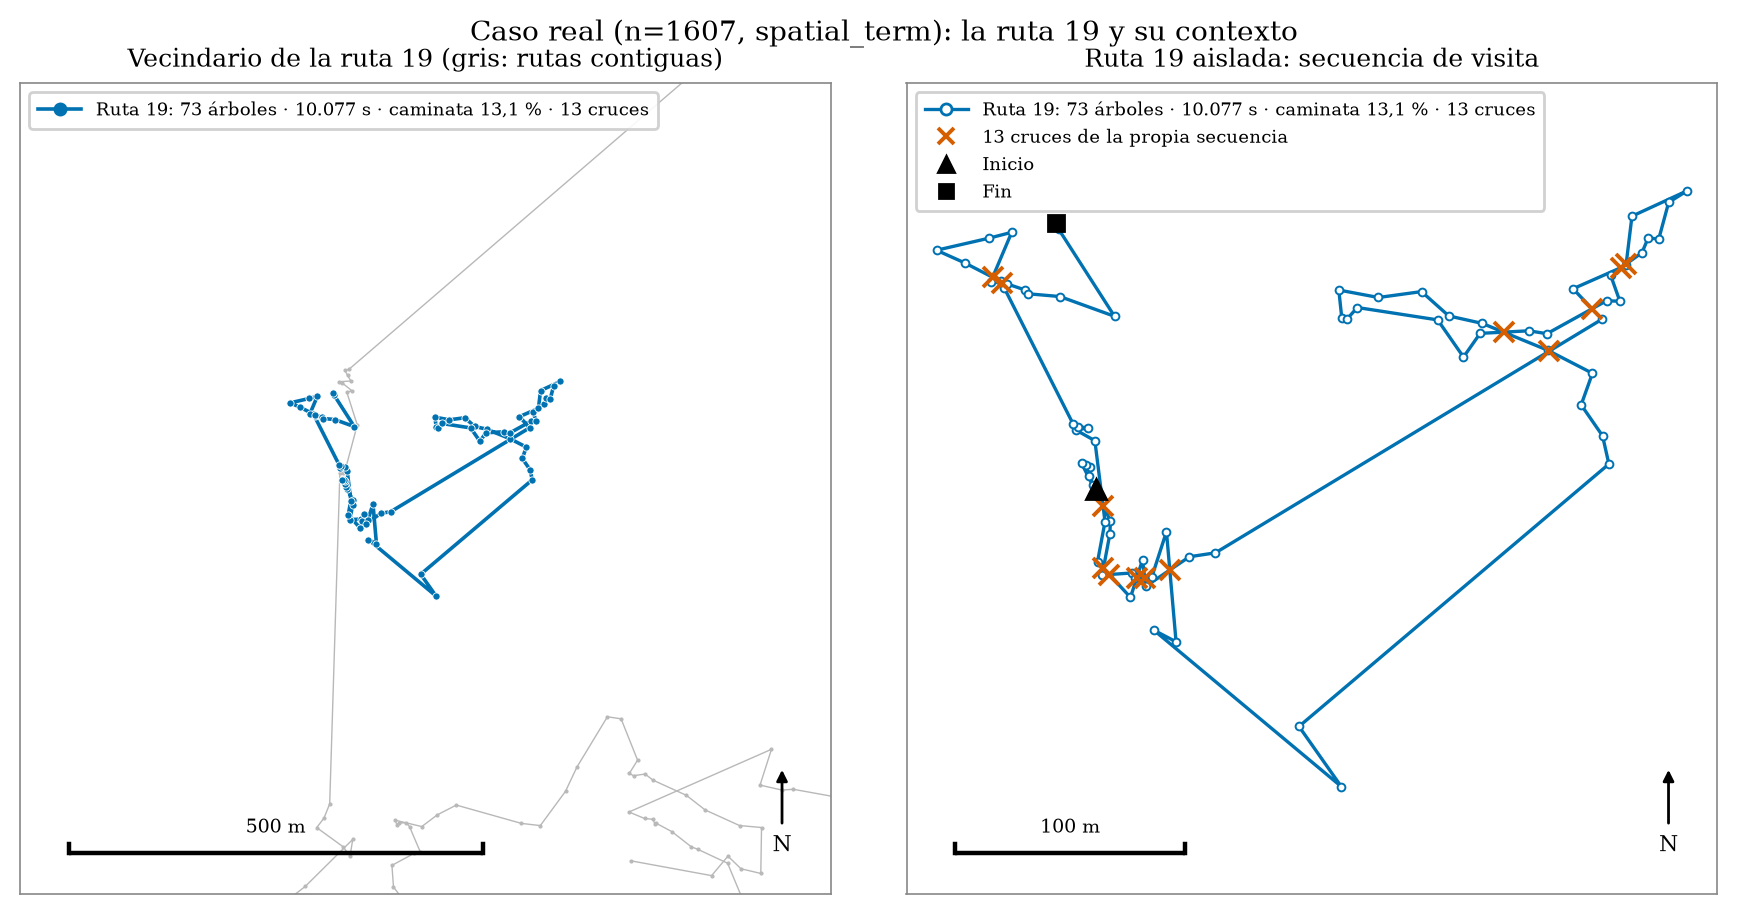
\includegraphics[width=0.9\textwidth]{media/fig-ruta-vueltas-r1.png}
  \caption{Ruta con auto-cruces en el \textit{dataset} de evaluación
    ($n = 1\,607$, estrategia \texttt{spatial\_term}, configuración de producción).
    El cruzamiento refleja la extensión del conjunto agregado, sin correlato
    operativo en el censo histórico, no una limitación de la formulación.}
  \label{fig:ruta-vueltas-r1}
\end{figure}

\begin{figure}[H]
  \centering
  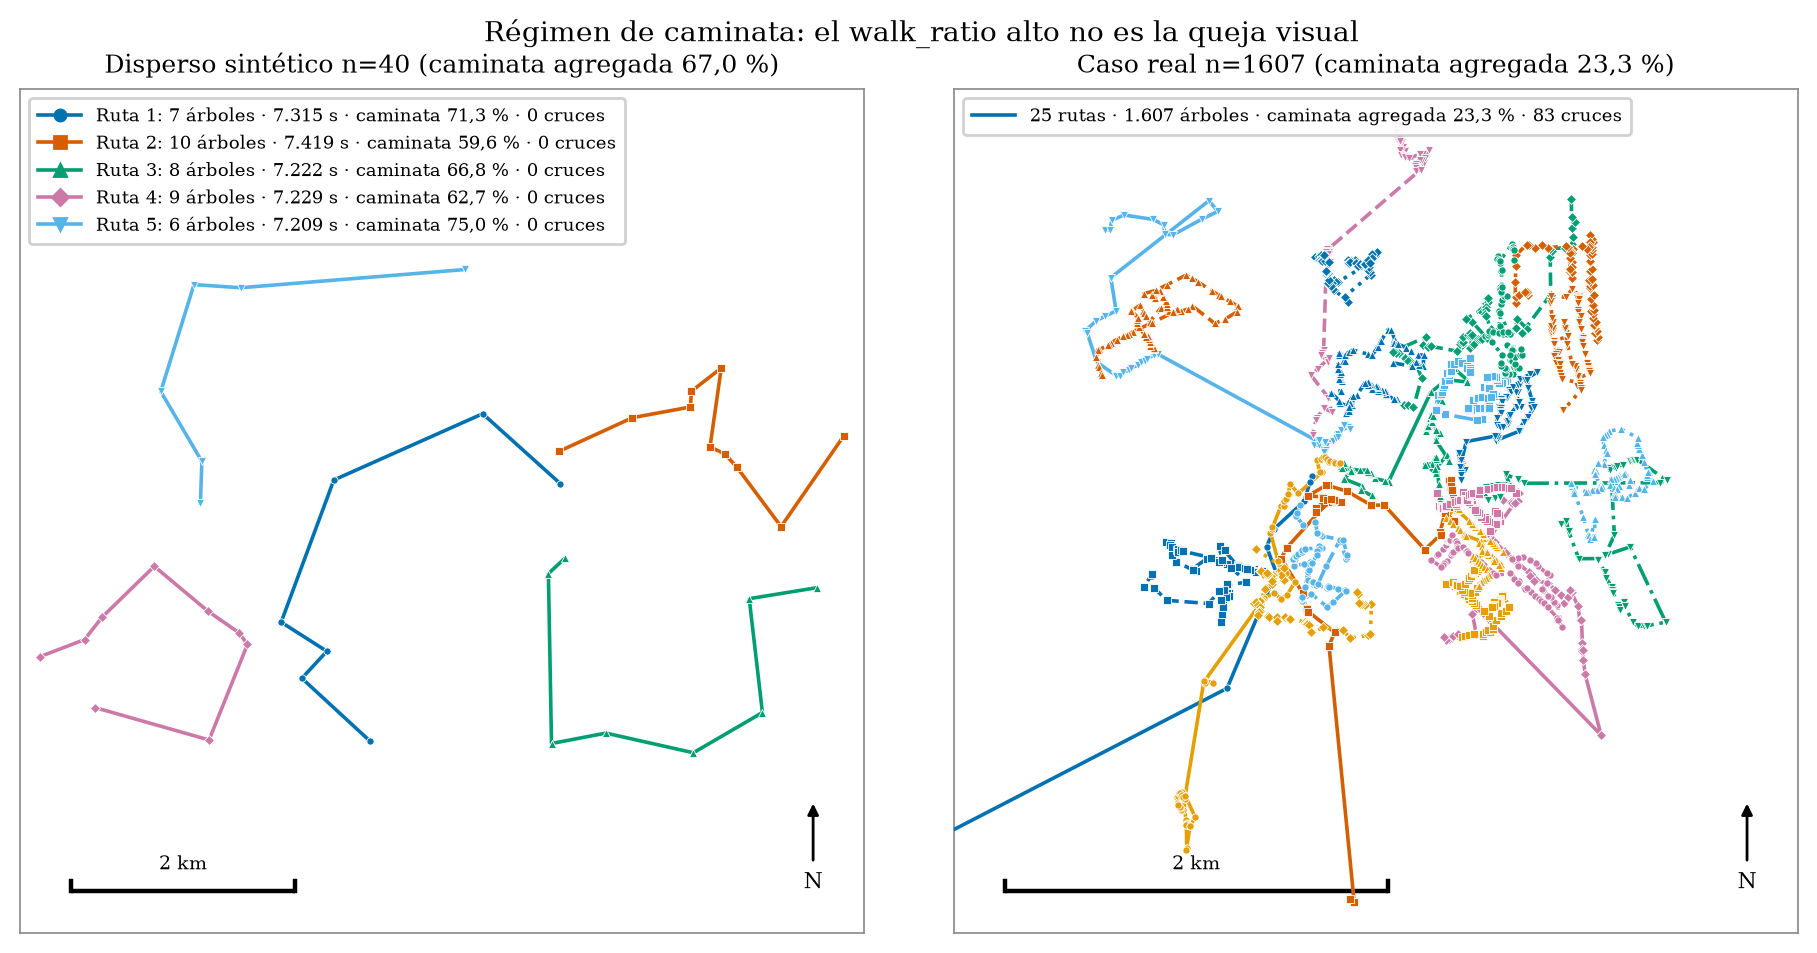
\includegraphics[width=0.9\textwidth]{media/fig-regimen-disperso-vs-real.png}
  \caption{Régimen disperso (extensión $\approx 10{,}3$\,km, \textit{dataset} de
    evaluación agregado) frente a régimen real (extensión $\leq 1{,}32$\,km, áreas
    individuales del arbolado legado). En el régimen real la configuración de
    producción genera rutas sin auto-cruces.}
  \label{fig:regimen-disperso-vs-real}
\end{figure}

\begin{figure}[H]
  \centering
  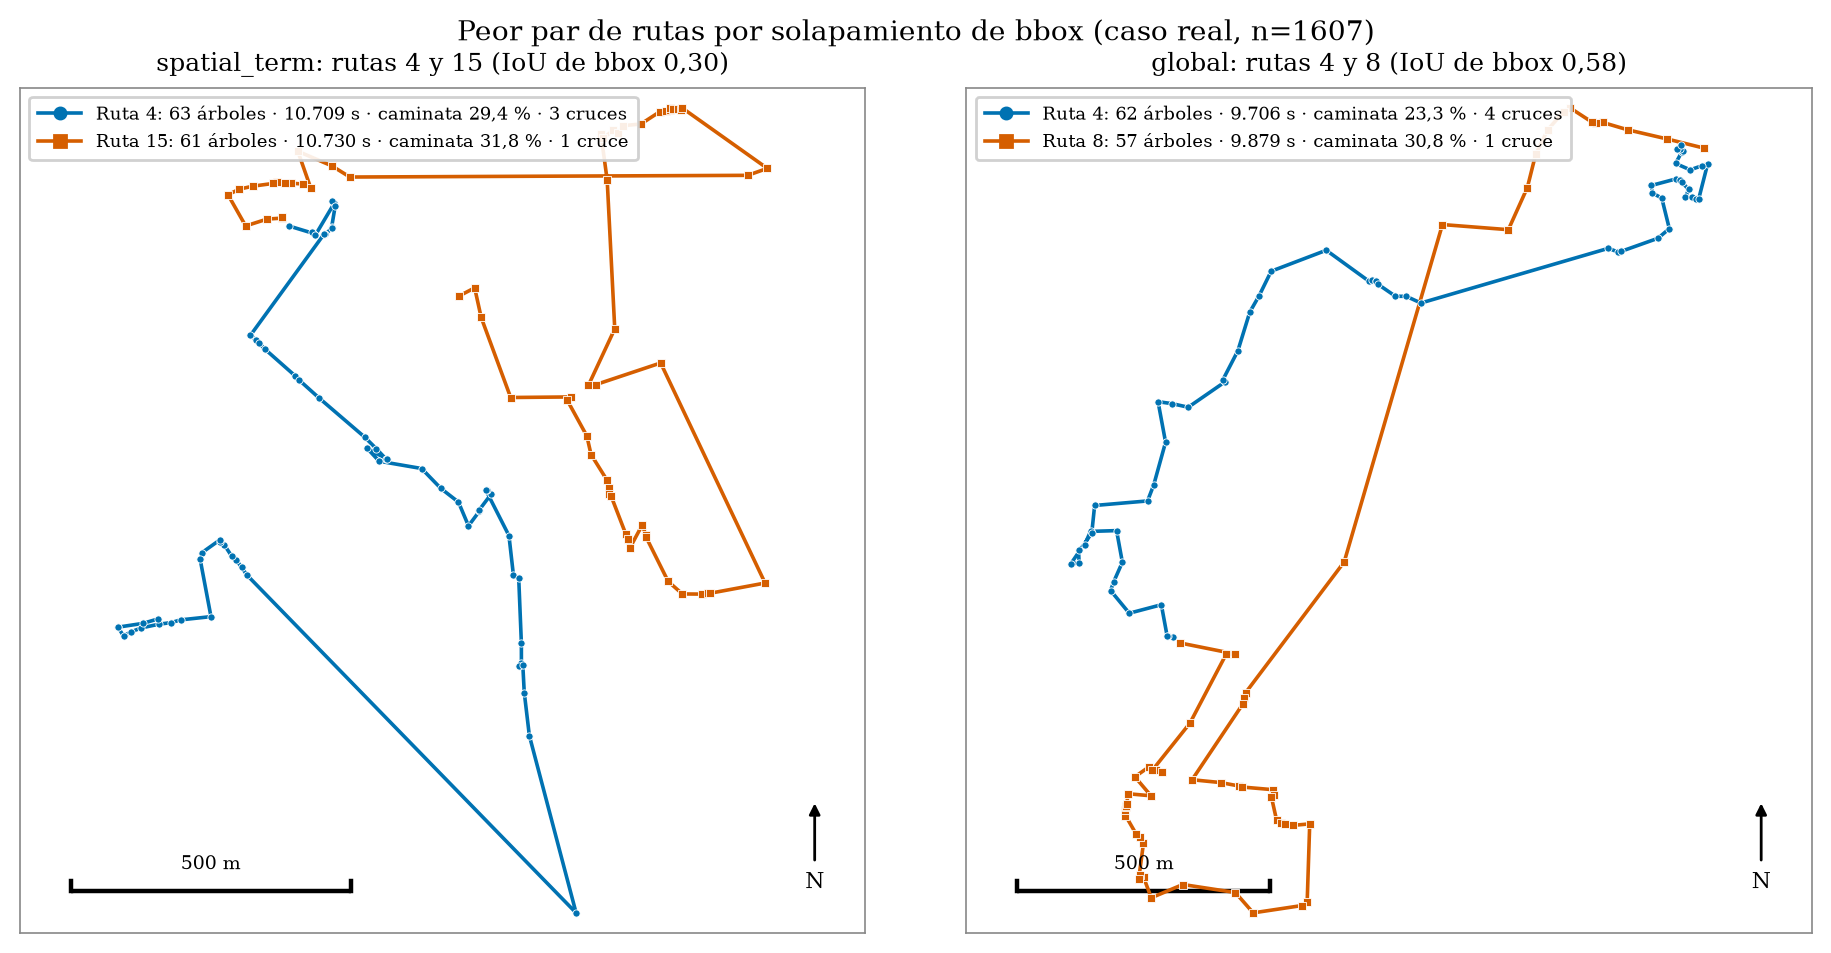
\includegraphics[width=0.9\textwidth]{media/fig-peor-par.png}
  \caption{Par de rutas con mayor solapamiento espacial
    (\textit{IoU} del peor par $= 0{,}55$) en el \textit{dataset} de evaluación.
    El solapamiento persiste con la estrategia \texttt{spatial\_term} porque responde
    a la geometría local del par, y ningún coeficiente global lo elimina sin penalizar
    las rutas circundantes.}
  \label{fig:peor-par}
\end{figure}

De los resultados anteriores se derivan dos respuestas directas a las preguntas de
evaluación más frecuentes. La pregunta «¿por qué las rutas no se ven compactas
visualmente?» tiene respuesta en la geometría: la configuración de producción produce
rutas sin auto-cruces en áreas de extensión real ($\leq 1{,}32$\,km), y cuando los auto-cruces
aparecen responden a la función objetivo, no a una limitación del tiempo de cómputo.
La pregunta «¿por qué el \textit{baseline} greedy se acerca en desplazamiento total?»
tiene respuesta en la saturación: el heurístico llena cada ruta hasta un $98$\,\%
de $T_{\max}$ ---sin dejar holgura operacional--- de modo que su reducción de caminata
proviene de la cota, no de la calidad del ordenamiento. La diferencia de $4{,}8$\,\%
de desplazamiento a favor del \textit{solver} ---medida contra un \textit{baseline}
que recibe el mismo post-pass de 2-opt--- y la menor severidad de su ruta residual son
las dimensiones que el tiempo total de
desplazamiento no captura de forma aislada (Sección~\ref{sec:comparacion-estrategias}).

La unidad operativa del motor es el área de censo individual, no el arbolado
metropolitano en su conjunto. Procesar cada área como un problema independiente
reduciría la extensión del \textit{dataset} a la escala en que el \textit{solver}
produce rutas limpias con la configuración actual; esa extensión se documenta como
trabajo futuro en la Sección~\ref{sec:posibles-mejoras} y su costo se midió
después sobre las áreas reales (Sección~\ref{sec:areas-reales}), donde resulta ser
una ruta adicional y el triple de cómputo, no kilómetros de caminata. El problema que esa extensión
plantea ---repartir un territorio en distritos compactos y equilibrados antes de
rutear--- tiene tratamiento propio en la literatura bajo la denominación de diseño
territorial \citep{kalcsics2005towards,rios2009reactive}, cuyos criterios de
compacidad y de balance coinciden con los dos ejes que esta sección mide.

Para confirmar el origen de los auto-cruces en la función objetivo y explorar si existe
una configuración universal, se ejecutó un barrido de configuración $\times$ algoritmo
$\times$ tamaño sobre la suite de instancias congeladas
(\texttt{route-config-algorithm-sweep-20260718.csv}; 96 celdas ---ocho
configuraciones sobre 12 instancias, $43 \leq n \leq 1\,607$--- registradas en
288 filas). Cada celda se registró con tres repeticiones nominales, pero el
comando de gestión que ejecutó el barrido escribía la semilla en el CSV sin
propagarla al \textit{solver}, de modo que las tres filas de una misma celda no
son réplicas independientes: difieren solo por el corte por reloj de pared
descrito en la Sección~\ref{sec:metricas-calidad}. En 78 de las 96 celdas las
tres filas coinciden exactamente; en las 18 restantes el desplazamiento total
varía hasta un $3{,}4$\,\%. Las cifras que siguen provienen, por tanto, de una
medición por celda sin réplica de semilla y no llevan barras de error.

El brazo \texttt{upper-tmax-tmin9000} ---que ancla la penalización blanda superior en
$T_{\max}$ en lugar del punto medio del intervalo $[T_{\min},\,T_{\max}]$ y eleva el
piso blando a $9\,000$\,s--- es el único que satisface el criterio de decisión para
$n=1\,607$: los auto-cruces caen un $92{,}5$\,\% ($89{,}0 \to 6{,}7$) con una variación de
viaje de $-0{,}3$\,\%, balance de $0{,}84$, $k=25$ y cero descartes. La razón es
estructural: a esa densidad las rutas saturan el presupuesto temporal de forma natural
($\overline{\text{sat}} = 0{,}94$), de modo que anclar la cota superior en $T_{\max}$ no
impone \textit{detours} adicionales. En el eje de algoritmo, \texttt{global} prácticamente no
modifica los auto-cruces ($-2{,}6$\,\%) y \texttt{greedy} los empeora ($+14{,}6$\,\%), lo que
ratifica \texttt{spatial\_term} como la estrategia correcta.

Sin embargo, el mismo brazo produce el peor resultado en las áreas reales individuales,
donde la instancia no satura $T_{\max}$ ($\overline{\text{sat}} \approx 0{,}67$--$0{,}73$):
anclar la cota superior fuerza relleno de trayecto porque la carga de servicio disponible
no llena el presupuesto, con incrementos de viaje de $+64{,}0$\,\%, $+62{,}6$\,\% y
$+89{,}0$\,\% en las instancias de $n = 157$, $72$ y $43$, respectivamente. Bajo la
configuración de producción, esas mismas áreas generan cero o casi cero auto-cruces; el
auto-cruce es un fenómeno exclusivo del régimen denso agregado
(Ilustración~\ref{fig:regimen-disperso-vs-real}). El brazo \texttt{span-c100} ---penalización
del \textit{span} sobre la dimensión temporal mediante
\texttt{SetSpanCostCoefficientForAllVehicles}, que eleva el coeficiente de $0$ en
producción a $100$ y deja intacta la penalización de $3$ sobre la dimensión espacial---
confirma la predicción de nulidad: solo reduce los auto-cruces en $26{,}6$\,\% para
$n=1\,607$, por debajo del umbral del $30$\,\% exigido por el criterio a priori, porque
penalizar la suma de duraciones de ruta no distingue el relleno del viaje productivo.
Los brazos que reducen o suprimen el piso blando
(\texttt{tmin-scaled}, \texttt{service-floor} y \texttt{tmin-scaled+exempt-last}) quedan
descalificados como configuración universal al romper la compuerta de balance $\geq 0{,}80$
en siete, siete y cuatro instancias, respectivamente.

La conclusión del barrido es que no existe una configuración única ganadora para todos los
regímenes sin una compuerta previa: la hipótesis queda refutada. El escenario donde
\texttt{upper-tmax-tmin9000} produce una ganancia decisiva ---el conjunto de evaluación
agregado de $n=1\,607$--- es una instancia agregada sin correlato operativo en el censo
histórico, que se organizó por área. Esa instancia no queda descartada: representa el
régimen de escalamiento ---un censo de cobertura mayor, o el ruteo de una comuna
completa como un solo problema---, pero no la unidad operativa histórica.
La decisión adoptada es conservar la configuración de producción (\texttt{actual}) sin
modificación y publicar \texttt{upper-tmax-tmin9000} como propuesta verificada para un
\textit{guard} por saturación a priori ($\overline{\text{sat}} \gtrsim 0{,}9$, cuantificado
a partir del CSV del barrido): el código de los \textit{overrides} queda en el árbol
(opt-in, producción intacta) para habilitar ese \textit{guard} cuando se implemente el
selector, extensión que se documenta como trabajo futuro en la
Sección~\ref{sec:posibles-mejoras}.

\subsubsection*{Auditoría de robustez metodológica}

La serie experimental descrita registra dieciséis ciclos de evaluación cerrados durante
julio de 2026. El análisis retrospectivo de esa evidencia identificó cuatro defectos de
instrumentación en los ciclos iniciales. Primero, el manejo de semillas en las corridas
iniciales (\#194 a \#217) no propagaba la semilla al \textit{solver}: las nominales tres
réplicas por celda eran la misma corrida, de modo que la dispersión reportada
($\sigma \approx 0{,}03\,\%$) es artefacto de replicación idéntica y no describe la
convergencia del algoritmo. Una corrida de recalibración (\#221) propagó semillas reales
al \textit{solver}, con lo que la dispersión subió a $\sigma \approx 2{,}4\,\%$ y catorce
de veintiocho veredictos de ese ciclo debieron re-juzgarse. Segundo, la métrica de relleno
en esos mismos ciclos usaba como cota inferior el producto $n \times \bar{n}$, que viola la
restricción de grado de los caminos y por tanto resulta inalcanzable. La métrica corregida
usa el bosque generador mínimo $\text{MSF}_k$, que es una cota válida y alcanzable.

Tercero, la métrica de auto-cruces se calcula sobre cuerdas rectas entre paradas
consecutivas (Sección~\ref{sec:posibles-mejoras}), una geometría que no coincide ni con
la red que el \textit{solver} optimiza ni con la polilínea real que se dibuja al censista.
Una validación posterior (\#240 y \#241) midió la correlación entre cuerdas y trazado real
de calles: $\rho$ de Spearman global de 0{,}527, propia de un indicador indirecto parcial,
e invertida en el \textit{dataset} de evaluación principal ($\rho = -0{,}575$). La prueba
decisiva es que el aumento de auto-cruces atribuido al 2-opt intra-ruta, que sobre cuerdas
se multiplicaba por 2{,}9 a 5{,}3 veces, se convierte sobre la geometría real de calles en
una reducción o un empate en 104 de 108 filas comparadas, con aumento en solo cuatro.
La métrica de cuerdas conserva, no obstante, su valor comparativo: dentro de cada ciclo
todos los brazos se contrastaron con la misma vara, de modo que las diferencias relativas
permanecen válidas aunque el nivel absoluto quede acotado por esta limitación.

Cuarto, el criterio de rutas degeneradas mezcla dos fenómenos: un aislamiento geográfico
que captura el conteo de paradas (menos de cinco) y un perjuicio operativo real que captura
la duración (menos de 1\,800 segundos). Una ruta con tres paradas y 10\,485\,s de duración
ocupa el 97\,\% del presupuesto diario y constituye una jornada completa, aunque viole el
conteo. La revisión del criterio descartó la cláusula de paradas por indirecta, con lo que
cuarenta y cinco de las ciento seis filas re-juzgables quedan absueltas y sesenta y una
persisten por duración.

Estas correcciones se originaron dentro de la propia serie y no invalidan sus conclusiones:
de los dieciséis ciclos, uno queda con el veredicto impugnado, dos se releyeron con el
instrumento corregido sin que cambiara el descarte final y los demás descansan en criterios
—tiempo de viaje, relleno, balance— ajenos a los defectos detectados. El caso de mayor
alcance es el 2-opt intra-ruta, rechazado en \#196 por empeorar los auto-cruces medidos en
cuerdas: la validación de \#240 y \#241 mostró que ese empeoramiento era artefacto de la
métrica y que el algoritmo limpia la geometría real. Sobre esa base, el ciclo \#245 lo
incorporó a la configuración de producción, con reducción simultánea de tiempo de viaje y
de auto-cruces sobre calle en las doce instancias de prueba y sin degradar el balance ni el
número de rutas. Es el único cambio de configuración por defecto de toda la serie, y no
proviene de barrer términos de la función objetivo sino de corregir el instrumento de
medición. El análisis completo se documenta en
\texttt{docs/experiments/evidence-audit-20260724.md}.

\section{PERFIL DE RENDIMIENTO DEL OPTIMIZADOR}
\label{sec:perfil-rendimiento}

Esta sección caracteriza el comportamiento temporal del motor de optimización:
en qué fases del \textit{pipeline} se concentra el tiempo de ejecución, cómo
varían las soluciones ante los parámetros operacionales (tiempo de servicio por
árbol y cota dura $T_{\max}$) y cuál es la sensibilidad del sistema al tamaño
del problema y al presupuesto del \textit{solver}. Todas las cifras provienen del
experimento de perfilado ejecutado el 11--12 de julio de 2026, cuyo protocolo y
datos crudos se encuentran versionados en el directorio
\texttt{docs/experiments/} del repositorio (reporte
\texttt{profiling-20260711.md} y archivos CSV asociados), y son reproducibles
mediante el comando de gestión \texttt{baseline\_sweep}, verificado
previamente sobre una corrida sintética de $n=80$
(\texttt{baseline-sweep-20260711.md}).

Corresponde advertir que las cifras de esta sección provienen de un
régimen de medición anterior al de la
Sección~\ref{sec:comparacion-estrategias}: se obtuvieron con la estrategia
\texttt{global}, un límite de \textit{solver} de 180\,s y una versión del código previa a
la corrección del redondeo del tránsito (el truncamiento entero descrito al
final de la Sección~\ref{sec:variantes-duracion}). Ese era el régimen vigente en
producción al momento del perfilamiento, y son sus propios resultados los que lo
dejaron obsoleto: el análisis de sensibilidad de la
Tabla~\ref{tab:sensibilidad-tl} es el que motivó bajar el límite de \textit{solver} de
180 a 120\,s, mientras que la adopción de \texttt{spatial\_term} como estrategia
por defecto proviene del experimento de comparación de la
Sección~\ref{sec:comparacion-estrategias}. El perfil documenta, por tanto, el
estado previo a ambas decisiones y no se reejecutó bajo el régimen nuevo: sus
tablas ---en particular la grilla de seis variantes de la
Tabla~\ref{tab:grilla-variantes}--- no deben cruzarse arco a arco con
las de la Sección~\ref{sec:comparacion-estrategias}, por las razones que allí se
detallan. La sección se conserva porque sus hallazgos son de \textit{tiempo}
---la dominancia del GLS y el carácter \textit{OSRM-bound} en frío---, que no
dependen de la estrategia ni del redondeo, y porque el barrido de la
Tabla~\ref{tab:sensibilidad-tl} trata el presupuesto de \textit{solver} como variable del
experimento y no como constante del régimen.

\subsection{Entorno de medición}

Dado que el sistema no cuenta con un despliegue productivo, las mediciones se
realizaron sobre una réplica local del entorno de producción definida en
\texttt{docker-compose.prod.yml}: imágenes construidas con el \textit{target}
\texttt{prod} del \texttt{Dockerfile} (sin \textit{bind-mounts} de código ni
recarga en caliente, con usuario no privilegiado), una instancia real de OSRM
cargada con el extracto completo de Chile de \textit{OpenStreetMap}
(\texttt{chile-latest.osm.pbf}), preprocesado con el algoritmo
\textit{Multi-Level Dijkstra} (MLD) \citep{delling2017customizable} y perfil
peatonal, además de PostGIS \citep{postgis} 15--3.3 y Redis 7. Las versiones
empleadas fueron Python 3.12.11, Django \citep{django} 6.0, \textit{OR-Tools}
\citep{ortools} 9.15 y NumPy 2.4.6.

Este entorno difiere de un despliegue real en tres aspectos que deben
considerarse al interpretar las cifras absolutas: (i) el hardware es un Apple
M4 Pro (arm64, 12 núcleos, 24\,GB) bajo Docker Desktop, con los contenedores de
base de datos y OSRM emulados en \texttt{linux/amd64} mediante Rosetta,
mientras que un servidor de producción típico sería x86 nativo con recursos
menores; (ii) la comunicación con OSRM y la base de datos ocurre por la red
interna de \textit{compose} en la misma máquina, con latencia cercana a cero,
mientras que en un centro de datos la latencia de red encarecería la fase de
consulta a OSRM (100 solicitudes HTTP para $n=1\,607$); y (iii) el punto de
entrada fue el comando de gestión ejecutado secuencialmente dentro del
contenedor, en lugar del flujo API~$\rightarrow$~Celery del sistema en
operación; ambos recorren el mismo código
(\texttt{OptimizationPipeline.run}), por lo que la diferencia agrega
únicamente latencia de encolado, no de cómputo.

\subsection{Desglose de tiempo por fase}

El \textit{pipeline} se instrumentó por fases: construcción de la matriz de
costos (\texttt{cost\_matrix}), construcción del modelo
(\texttt{model\_build}), resolución (\texttt{solve}, subdividida en primera
solución y metaheurística), extracción de la solución
(\texttt{solution\_extraction}) y cálculo de métricas (\texttt{metrics}). El
hallazgo central es que el perfil depende del estado de la caché de la matriz
de distancias: en operación normal (caché caliente) el \textit{pipeline} está
acotado por el \textit{solver} (\textit{solve-bound}), y solo en el primer contacto con
un \textit{dataset} está acotado por OSRM (\textit{OSRM-bound}).

Con la caché caliente, la metaheurística \textit{Guided Local Search} (GLS)
concentra el 98,1\,\% del tiempo total, y todas las demás fases combinadas
representan menos del 2\,\% (Tabla~\ref{tab:fases-caliente}). Optimizar la
construcción del modelo, la extracción o el cálculo de métricas no tendría,
por tanto, ningún efecto medible.

\begin{table}[H]
  \centering
  \caption{Desglose de tiempo por fase con caché de matriz caliente ($n=1\,607$; media de las 18 corridas de la grilla).}
  \label{tab:fases-caliente}
  \begin{tabularx}{\textwidth}{lXX}
    \toprule
    Fase & Tiempo [s] & \% del total \\
    \midrule
    \texttt{cost\_matrix} (consulta de caché) & 0{,}57 & 0{,}5\,\% \\
    \texttt{model\_build} & $<0{,}01$ & $\approx 0$\,\% \\
    \texttt{solve} (primera solución) & 1{,}4 & 1{,}3\,\% \\
    \texttt{solve} (metaheurística GLS) & 103{,}4 & \textbf{98{,}1\,\%} \\
    \texttt{solution\_extraction} & 0{,}01 & $\approx 0$\,\% \\
    \texttt{metrics} & 0{,}02 & $\approx 0$\,\% \\
    \midrule
    Total del \textit{pipeline} & 105{,}4 & 100\,\% \\
    \bottomrule
  \end{tabularx}
\end{table}

En frío ---caché de matriz vacía, primera corrida sobre el \textit{dataset}---
el perfil se invierte: la consulta a OSRM domina con el 97,6\,\% del tiempo
(Tabla~\ref{tab:fases-frio}). Para $n=1\,607$ la fragmentación por longitud de
URL (175 coordenadas por bloque) convierte la matriz en una grilla de
$10 \times 10 = 100$ solicitudes al servicio \texttt{/table}, con un costo
total de 170,8\,s que escala aproximadamente como $O(n^2)$ con el número de
celdas. Este costo se paga una única vez por \textit{dataset}: la matriz queda
almacenada en caché (indexada por el hash SHA-256 de los identificadores de
árboles activos), de modo que toda corrida posterior es \textit{solve-bound}.

\begin{table}[H]
  \centering
  \caption{Desglose de tiempo por fase en frío (caché de matriz vacía; corrida piloto con tiempo de servicio de 2\,min y $T_{\max}=3$\,h).}
  \label{tab:fases-frio}
  \begin{tabularx}{\textwidth}{lXX}
    \toprule
    Fase & Tiempo [s] & \% del total \\
    \midrule
    \texttt{cost\_matrix} (consulta OSRM) & 170{,}8 & \textbf{97{,}6\,\%} \\
    \texttt{cost\_matrix} (ensamblado y caché) & 0{,}2 & 0{,}1\,\% \\
    \texttt{solve} & 3{,}9 & 2{,}2\,\% \\
    Fases restantes & $<0{,}05$ & $\approx 0$\,\% \\
    \midrule
    Total del \textit{pipeline} & 174{,}9 & 100\,\% \\
    \bottomrule
  \end{tabularx}
\end{table}

Cabe notar que en la corrida piloto de la Tabla~\ref{tab:fases-frio} el GLS
terminó a los 3,9\,s; en la grilla completa el tiempo de resolución observado
para el mismo \textit{dataset} varió entre 29 y 180\,s, según si la búsqueda
agota o no el presupuesto de tiempo asignado.

\subsection{Variaciones de duración sobre el \textit{dataset} real}
\label{sec:variantes-duracion}

Se evaluaron las seis combinaciones de tiempo de servicio por árbol
$\{1, 2, 3\}$\,min y cota dura $T_{\max} \in \{2, 3\}$\,h, con
$T_{\min} = \min(7\,200\,\text{s}, T_{\max})$, sobre el \textit{dataset} real
completo de $n=1\,607$ árboles (429 provenientes de la fuente
\texttt{legacy\_api} y 1\,178 de \texttt{legacy\_app}, estas últimas con
posición mediana por código QR). Cada variante se ejecutó con 3 semillas y un
límite de \textit{solver} de 180\,s, que era el tope vigente en producción al momento de
este perfilamiento ($\min(30 + 1{,}5 \cdot n,\ 180)$ para ese tamaño); el tope
se bajó a 120\,s justamente a partir del análisis de sensibilidad de la
Tabla~\ref{tab:sensibilidad-tl}.
La Tabla~\ref{tab:grilla-variantes} resume las medias por variante.

\begin{table}[H]
  \centering
  \caption{Grilla de seis variantes sobre el \textit{dataset} real ($n=1\,607$; media de 3 semillas; límite de \textit{solver} de 180\,s). El total del \textit{pipeline} equivale al tiempo de \texttt{solve} más $\approx$0{,}6\,s de sobrecosto fijo.}
  \label{tab:grilla-variantes}
  \small
  \begin{tabularx}{\textwidth}{rrXXXXXXX}
    \toprule
    Serv. [min] & $T_{\max}$ [h] & $k$ & Balance & $\bar{T}$ [s] & $\sigma(T)$ [s] & Descart. & Des\-plaz. [s] & \texttt{solve} [s] ($\pm$\,sd) \\
    \midrule
    1 & 2 & 23{,}0 & 0{,}992 & 7\,229  & 14  & 0     & 69\,868 & 92{,}8 $\pm$ 63{,}8 \\
    1 & 3 & 15{,}0 & 0{,}877 & 10\,417 & 378 & 0     & 59\,843 & 89{,}0 $\pm$ 3{,}6 \\
    2 & 2 & 36{,}0 & 0{,}996 & 7\,219  & 6   & 0     & 67\,047 & 131{,}6 $\pm$ 34{,}4 \\
    2 & 3 & 24{,}0 & 0{,}865 & 10\,399 & 391 & 0     & 56\,750 & 126{,}9 $\pm$ 6{,}7 \\
    3 & 2 & 49{,}0 & 0{,}998 & 7\,213  & 3   & 1{,}0 & 64\,360 & 139{,}2 $\pm$ 14{,}1 \\
    3 & 3 & 33{,}0 & 0{,}890 & 10\,554 & 284 & 0     & 59\,023 & 49{,}3 $\pm$ 14{,}1 \\
    \bottomrule
  \end{tabularx}
\end{table}

Los resultados muestran el compromiso central entre balance y costo total. Con
$T_{\max}=2$\,h el número de rutas $k$ escala fuertemente con el tiempo de
servicio ($23 \rightarrow 36 \rightarrow 49$), pues el trabajo de servicio
domina la capacidad de cada ruta, y el balance se aproxima a 1
(al coincidir $T_{\min}$ y $T_{\max}$, las rutas resultan de duración casi
idéntica, con $\sigma(T)$ de 3 a 14\,s). Con $T_{\max}=3$\,h, en cambio, el
tiempo total de desplazamiento se reduce en torno al 10\,\% y $k$ cae
alrededor de un 35\,\%, a costa de un balance de $\approx 0{,}87$ con
$\sigma(T)$ de 284 a 391\,s. La única variante que descarta nodos es la más
restrictiva (servicio de 3\,min con $T_{\max}=2$\,h), que deja un árbol fuera
de la solución de forma consistente en las tres semillas.

Respecto de las semillas, corresponde precisar su rol: dados los parámetros,
el \textit{solver} de \textit{OR-Tools} es determinista, por lo que sobre el \textit{dataset}
real la semilla actúa únicamente como etiqueta de la repetición. La varianza
observada entre repeticiones (columna sd de \texttt{solve} en la
Tabla~\ref{tab:grilla-variantes}) proviene del corte por tiempo de reloj
(\textit{wall-clock}) del GLS: en las variantes en que la búsqueda agota el
presupuesto, las tres repeticiones convergen a soluciones casi idénticas.

Finalmente, la grilla registra rutas cuyo tiempo estimado excede $T_{\max}$
en la configuración de 2\,h (por ejemplo, la práctica totalidad de las rutas
en las variantes con servicio de 2 y 3\,min). Este exceso no constituye una
infactibilidad del \textit{solver}, sino un artefacto de redondeo: el \textit{callback}
de tránsito trunca cada arco a aritmética entera
(\texttt{int(travel + service)}), mientras que la métrica de duración estimada
suma los mismos términos en punto flotante; con 30 a 70 arcos por ruta, el
truncamiento acumula una discrepancia de 10 a 70\,s por ruta. La cota dura
$T_{\max}$ se respeta estrictamente en la aritmética entera del \textit{solver}.

\subsection{Sensibilidad al tamaño del problema y al presupuesto del solver}

Para aislar el efecto del tamaño del problema se repitió la grilla sobre un
área reducida del mismo origen legado ($n=157$). La fase que peor escala es la
consulta a OSRM en frío: de 1,7\,s con $n=157$ a 170,8\,s con $n=1\,607$
---un factor de $\approx 100\times$ para $10\times$ el número de nodos,
consistente con el crecimiento $O(n^2)$ del número de celdas de la matriz---.
La primera solución del \textit{solver} pasa de 0,02\,s a 1,4\,s ($\approx 63\times$).
La metaheurística, en cambio, no escala de forma monótona con $n$ a presupuesto
fijo: con $n=157$ el GLS agota los 180\,s en casi todas las variantes (media de
167\,s), mientras que con $n=1\,607$ corta antes en varias (media de 103\,s).
El límite de tiempo de reloj enmascara el costo por iteración: lo que crece con
$n$ es el costo de explorar cada vecindario, no el tiempo total observado.

Dado que el GLS domina el tiempo en operación normal, su presupuesto es el
parámetro de operación relevante. La Tabla~\ref{tab:sensibilidad-tl} muestra la
sensibilidad de la calidad de la solución al límite de tiempo para la variante
central (servicio de 2\,min, $T_{\max}=3$\,h, $n=1\,607$): el número de rutas y
el balance quedan fijos desde los 60\,s, y la mejora de desplazamiento total
entre 120\,s y 180\,s es de solo 0,1\,\%. Un límite de 120\,s captura por tanto
$\approx 99$\,\% de la mejora alcanzable con 180\,s, lo que permitiría reducir
el costo de cada corrida de producción en un tercio sin pérdida de calidad
medible.

\begin{table}[H]
  \centering
  \caption{Sensibilidad al límite de tiempo del \textit{solver} (servicio de 2\,min, $T_{\max}=3$\,h, $n=1\,607$).}
  \label{tab:sensibilidad-tl}
  \begin{tabularx}{\textwidth}{rXXXX}
    \toprule
    Límite [s] & $k$ & Balance & Desplaz. total [s] & $\Delta$ desplaz. vs.\ 60\,s \\
    \midrule
    60  & 24 & 0{,}867 & 61\,521 & --- \\
    120 & 24 & 0{,}865 & 56\,830 & $-7{,}6$\,\% \\
    180 & 24 & 0{,}865 & 56\,750 & $-7{,}8$\,\% \\
    \bottomrule
  \end{tabularx}
\end{table}

\section{CONCLUSIONES}
\label{sec:conclusiones}

\subsection{Cumplimiento de los criterios de aceptación}

Los seis criterios comprometidos en la Sección~\ref{sec:criterios-aceptacion}, antes
de ejecutar experimento alguno, se contrastan aquí contra lo medido. Cinco se cumplen
y el sexto se cumple con una reserva de protocolo que corresponde declarar.

La cobertura del censo (CA-01) es total bajo la configuración censal de referencia:
las tres repeticiones de la corrida de referencia asignan los $1\,607$ árboles a una
ruta, sin que el modelo active la disyunción que le permitiría descartarlos. El
criterio deja de cumplirse únicamente cuando la carga de servicio excede la capacidad
de la flota bajo $T_{\max}=2$\,h, y esa frontera está caracterizada en la
Tabla~\ref{tab:grilla-spatial}. La jornada máxima (CA-02) se respeta sin excepción:
la cota es dura por construcción del modelo, y la corrección del redondeo del tránsito
eliminó el artefacto de medición que antes producía excesos aparentes. El balance de
carga (CA-03) queda holgadamente dentro del criterio, con una desviación estándar de
$559$\,s equivalente al $5{,}6$\,\% del promedio frente al $15$\,\% exigido. La flota
(CA-04) es en efecto una salida del sistema: el administrador declara la duración de
la jornada y el tiempo de servicio, y el número de censadores necesarios se deriva de
ellos, lo que constituye la diferencia funcional más nítida respecto de la
planificación manual descrita en la Sección~\ref{sec:solucion}.

El costo de cómputo (CA-05) se cumple, pero su lectura exige una precisión: los
$120$\,s medidos son el tope configurado del \textit{solver} y no una medición de
convergencia, de modo que el criterio se satisface por construcción mientras el tope
se mantenga bajo cinco minutos. Lo que sí constituye evidencia es el análisis de
sensibilidad de la Tabla~\ref{tab:sensibilidad-tl}, que muestra que ese tope captura
prácticamente toda la mejora alcanzable con presupuestos mayores, y el desglose por
fases, que sitúa el $98{,}1$\,\% del tiempo en la metaheurística y no en la
infraestructura que la rodea.

La mejora sobre la alternativa trivial (CA-06) se cumple con un margen menor que el
que se reportó en una primera medición. Aquella restaba cifras de corridas distintas
sobre reconstrucciones del mismo conjunto de árboles ---y el heurístico es sensible al
orden interno de los nodos, que difería entre ellas--- y comparaba la solución del
\textit{solver}, que recibe el post-proceso de resecuenciación de la
Sección~\ref{sec:postpass}, contra un \textit{baseline} sin refinamiento local alguno.
Repetido el experimento con las tres columnas sobre la misma instancia congelada y con
el heurístico dotado del mismo post-proceso (Tabla~\ref{tab:comparativa}), el ahorro
resulta ser de $2\,907$\,s, un $4{,}8$\,\% del desplazamiento total del
\textit{baseline} refinado, en lugar del $6{,}7$\,\% inicial: alrededor de un tercio de
aquel margen era atribuible al post-proceso que solo un lado recibía. El margen
subsistente supera la dispersión entre semillas del \textit{solver} ($1\,538$\,s), de
modo que el criterio se cumple. Junto a él subsiste una diferencia cualitativa: el
\textit{baseline} produce una ruta degenerada de cinco árboles con $9\,466$\,s de
caminata y satura las jornadas a un promedio del $98$\,\% de $T_{\max}$, mientras que
la solución del modelo opera al $93$\,\% en promedio y su ruta más pequeña visita entre
seis y doce árboles. La atenuación de esa patología es de grado y no de naturaleza: el
modelo no la elimina.

\subsection{Lo que los resultados muestran sobre el problema}

Más allá del cumplimiento de los criterios, la serie de experimentos arroja un
hallazgo conceptual que no era la hipótesis de partida y que reorienta el problema.

La calidad geométrica de las rutas ---su compacidad, su solapamiento mutuo y sus
auto-cruces--- no es una propiedad del presupuesto de cómputo sino del régimen
geográfico de la instancia y de la forma de la función objetivo. Aumentar el tiempo
del \textit{solver} de 120 a 180\,s no cambia la geometría; redirigir el objetivo
blando superior sí la cambia de forma drástica, y hacerlo mejora la geometría en el
conjunto agregado a la vez que la empeora en las áreas individuales. Dicho de otro
modo: no existe una configuración de la función objetivo que sea la correcta para
todo tamaño y toda densidad, y la búsqueda de una ---la hipótesis con que se abrió el
barrido de configuración por algoritmo--- queda refutada con datos.

El corolario operacional es que la unidad correcta del problema es el área de censo
individual y no el arbolado metropolitano agregado. El conjunto de evaluación de
$n=1\,607$ árboles abarca $10{,}3$\,km de extensión, frente a los $1{,}32$\,km del
área real mayor, y es en ese régimen disperso ---y solo en él--- donde emergen los
auto-cruces que motivaron buena parte de la experimentación. Sobre un área real, la
configuración de producción ya genera rutas limpias. Esto convierte la segmentación
previa por área, que la Sección~\ref{sec:posibles-mejoras} documenta como trabajo
futuro, en la extensión de mayor impacto del sistema: no porque el motor esté mal
calibrado, sino porque el motor se comporta como corresponde cuando el problema se le
entrega en su escala natural.

El argumento dejó de ser solo geométrico cuando se midió sobre las áreas reales
(Sección~\ref{sec:areas-reales}). Particionar no cuesta caminata en el territorio
del censo histórico, porque las áreas están suficientemente separadas; cuesta una
ruta adicional, tres jornadas por debajo de $T_{\min}$ y el triple de cómputo, a
cambio de instancias con correlato operativo y de una varianza entre repeticiones
sustancialmente menor. Esa misma medición expuso el límite del \textit{solver} en
el otro extremo del rango: en un área de 72 árboles la búsqueda entrega dos medias
jornadas donde su propia función objetivo prefiere una jornada única por un factor
cercano a 43, de modo que el margen de mejora pendiente no está en los coeficientes
del objetivo sino en la búsqueda.

\subsection{Lo que aportó la metodología}

Dieciséis ciclos de evaluación cerrados produjeron un solo cambio en la configuración
por defecto del sistema. Leído a la ligera, eso parece un resultado nulo; leído con
propiedad, es el resultado.

Cada ciclo fijó su criterio de decisión antes de ejecutarse, versionó sus datos crudos
y publicó su veredicto con independencia de si confirmaba o refutaba la hipótesis que
lo motivaba. De los dieciséis ciclos, doce cerraron con un descarte ---pisos de
balance escalados y factibles, piso por número de paradas, piso combinado, supresión
del piso, anclaje del objetivo blando superior en $T_{\max}$, peso convexo y peso
lineal del arco, agrupamiento previo con restricción blanda, \textit{warm start},
multi-arranque y compuerta de régimen a priori---, dos fueron correcciones del propio
instrumento de medición, uno caracterizó la flojedad de la cota inferior de referencia
y uno adoptó un cambio. La conclusión que emerge del conjunto no es que no se encontró
nada, sino que la configuración de producción ya era la adecuada para su régimen de
operación, y que el margen de mejora que se le suponía a la función objetivo no
existía. Descartar doce alternativas plausibles con criterio pre-registrado es un
resultado más informativo que adoptar la primera que hubiera parecido prometedora.

El único cambio adoptado ---el post-proceso de resecuenciación de la
Sección~\ref{sec:postpass}--- refuerza esa lectura, porque no provino de barrer
términos del objetivo sino de reparar el instrumento de medición. El algoritmo había
sido rechazado por empeorar los auto-cruces medidos sobre cuerdas rectas; cuando la
validación posterior mostró que esa métrica está débilmente correlacionada con la
geometría real de calles ---y que en el \textit{dataset} de evaluación apunta en
sentido contrario---, la re-medición sobre el trazado real reveló una mejora
simultánea de tiempo de viaje y de geometría en las doce instancias de prueba. El
aprendizaje metodológico es transferible y vale más que el cambio concreto: en una
serie experimental larga, auditar el instrumento tiene mayor rendimiento esperado que
añadir un brazo más al barrido.

\subsection{Alcance y validez de lo concluido}

Las conclusiones anteriores valen dentro de un perímetro que conviene delimitar con
precisión, y que corresponde al alcance declarado en la Sección~\ref{sec:alcance} y a
las restricciones de la Sección~\ref{sec:restricciones}.

Valen sobre el arbolado real de las dos bases legadas del proyecto ---no sobre
instancias sintéticas ni sobre los bancos de referencia de la literatura
\citep{solomon1987algorithms}, que no se emplearon--- y sobre el rango de tamaños comprendido entre $43$ y $1\,607$ nodos. Las
comparaciones son internas: contrastan el sistema contra otras configuraciones de sí
mismo y contra un heurístico de vecino más cercano escrito para este trabajo. No hay
anclaje externo, ni una cota de optimalidad aplicada al resultado principal, de modo
que las afirmaciones son de mejora relativa y nunca de proximidad al óptimo.

Las cifras absolutas de tiempo provienen de un entorno de medición emulado y no de un
servidor de producción, y el sistema no fue desplegado ni operado en una jornada real
de censo. En consecuencia, lo verificado es que el producto hace lo que su diseño
declara ---en los términos de la Sección~\ref{sec:verificacion}--- y no que resuelva
en terreno el problema logístico que lo motivó. Esa última comprobación queda
pendiente y es, de todas las extensiones identificadas, la de mayor valor para el
proyecto.

Por último, dos reservas de instrumento acompañan a toda lectura de la geometría: la
métrica de auto-cruces se calcula sobre cuerdas rectas y su correspondencia con el
trazado real es parcial, y la replicación de los experimentos se obtiene permutando el
orden de los nodos, lo que acota la varianza entre semillas de una corrida pero no la
varianza entre corridas distintas. Ambas están cuantificadas en la auditoría de
robustez de la Sección~\ref{sec:discusion-calidad}, y ninguna de las dos afecta a los
criterios de aceptación ---cobertura, jornada, balance, flota y tiempo---, que
descansan en magnitudes ajenas a ellas.

\section{POSIBLES MEJORAS}
\label{sec:posibles-mejoras}

Entre las extensiones identificadas para versiones futuras del sistema se encuentran:

\begin{itemize}
  \item \textbf{Matrices de costos de gran escala}: superar el tope de $2\,000$ árboles que hoy acota la dimensión de la matriz de costos ---impuesto por el crecimiento $O(n^2)$ de su tamaño en disco--- mediante almacenamiento disperso o la segmentación previa del \textit{dataset}, para censos que excedan ese umbral.
  \item \textbf{Operación offline robusta}: reemplazar la cola offline básica actual (Sección~\ref{sec:ui}) por un \textit{service worker} que gestione el almacenamiento de teselas y la sincronización diferida de forma confiable en condiciones de conectividad intermitente.
  \item \textbf{Importación de formatos adicionales}: soporte de GeoJSON como formato de entrada de \textit{datasets}, que actualmente se importan desde archivos CSV o JSON, o bien desde las fuentes legadas (Sección~\ref{sec:legacy}).
  \item \textbf{Pruebas de extremo a extremo}: automatización de los flujos completos de administrador y censador mediante Playwright.
\end{itemize}

\subsection{Limitaciones del sistema}

Se documentan a continuación las limitaciones aceptadas en el alcance de esta
iteración de Arbocensus.

\begin{itemize}
  \item \textbf{Seguridad de sesión}: los tokens JWT se almacenan en
  \texttt{localStorage}, lo que simplifica la implementación a costa de una
  mayor exposición ante ataques de tipo \textit{cross-site scripting} en
  comparación con el almacenamiento en \textit{cookies} con atributo
  \texttt{HttpOnly}. El riesgo es aceptado para un sistema de intranet
  operado por personal interno.

  \item \textbf{Escala de la matriz de costos}: la matriz se construye por
  fragmentación (\textit{chunking}) en bloques cuando el \textit{dataset}
  supera las $350$ coordenadas que admite una única solicitud a OSRM
  (Sección~\ref{sec:matriz}), de modo que censos de miles de árboles ---como
  el conjunto de evaluación de $n = 1\,607$--- se procesan sin dificultad. El
  límite vigente es un tope de $2\,000$ árboles sobre la dimensión de la
  matriz, impuesto porque su tamaño en disco crece como $O(n^2)$; procesar
  \textit{datasets} que lo excedan requeriría almacenamiento disperso o la
  segmentación previa del arbolado.

  \item \textbf{Alcance del problema de ruteo}: el motor optimiza el
  \textit{dataset} completo como un único problema, sin segmentación previa
  por área geográfica. Cuando el \textit{dataset} reúne arbolado de múltiples
  áreas de censo ---como el conjunto de evaluación de $n = 1\,607$ árboles,
  que abarca $10{,}3$\,km de extensión en longitud--- las rutas resultantes
  reflejan esa extensión agregada, con los efectos de auto-cruce discutidos en la
  Sección~\ref{sec:discusion-calidad}. En la operación habitual, donde cada
  optimización corresponde a un área individual de extensión
  $\leq 1{,}32$\,km, esa limitación no se manifiesta; sin embargo, la
  plataforma no automatiza la segmentación previa por área, de modo que
  la correcta delimitación del \textit{dataset} de entrada recae en el
  administrador. Particionar el arbolado por área antes de rutear es la mejora
  de mayor impacto geométrico identificada para versiones futuras, y su costo
  está medido sobre las áreas reales (Sección~\ref{sec:areas-reales}): una ruta
  adicional, tres jornadas bajo $T_{\min}$ y el triple de cómputo, sin costo en
  desplazamiento.

  \item \textbf{Captura sin conectividad}: el portal de censo implementa una cola
  \textit{offline} básica mediante \texttt{persistQueryClient} sobre
  \textit{IndexedDB}, suficiente para preservar los datos ante pérdidas de conexión
  momentáneas; no se implementó un \textit{service worker} para la gestión de teselas
  de mapa ni para la sincronización diferida robusta bajo conectividad intermitente
  prolongada. Esa extensión se documenta en el apartado
  de posibles mejoras.

  \item \textbf{Accesibilidad de la base de datos legada}: la base de datos histórica del
  proyecto Arbocensus se encuentra activa en Heroku y se accede en modo de solo lectura
  para la importación de arbolado. Las fotografías de campo almacenadas en Firebase son
  inaccesibles por cierre del plan de facturación asociado; únicamente los metadatos y
  las coordenadas están disponibles para su uso en la plataforma.

  \item \textbf{Estrategia \texttt{cluster\_first}}: la estrategia de particionamiento
  previo mediante $k$-medias quedó descartada como opción de producción a partir de los
  resultados de la Sección~\ref{sec:comparacion-estrategias}. Incluso en su versión
  corregida, degrada el balance a $0{,}698$, incrementa el viaje en un $16{,}9$\,\% y
  descarta 12 árboles frente a \texttt{spatial\_term}, sin ventaja en ninguna dimensión
  que el criterio de decisión protege; se conserva en el código como opción de comparación
  para investigación, no como alternativa de censo.

  \item \textbf{Cobertura bajo presupuesto temporal estrecho}: la formulación admite
  descartes mediante disyunciones penalizadas ($1\,000\,000$\,s por árbol no cubierto),
  de modo que la cobertura total no está garantizada a priori cuando la carga de servicio
  excede la capacidad de la flota bajo $T_{\max}$. En la grilla de variantes operacionales,
  las configuraciones con $T_{\max}=2$\,h y tiempo de servicio alto descartan uno o dos
  árboles de forma consistente (Tabla~\ref{tab:grilla-spatial}); para garantizar cobertura
  total se requiere operar con $T_{\max}=3$\,h bajo esas condiciones.

  \item \textbf{Costo no medido de las disyunciones de nodos}: declarar cada árbol como
  una disyunción unitaria (Sección~\ref{sec:disyunciones}) añade una decisión binaria
  por nodo y amplía el vecindario que la búsqueda local debe explorar en cada
  iteración. Como el GLS se corta por reloj de pared y no por convergencia, cabe
  esperar que ese costo no se manifieste en un tiempo total mayor sino en una calidad
  menor alcanzable dentro del mismo presupuesto. La magnitud del efecto no se midió:
  aislarla exige una ablación con y sin disyunciones sobre el mismo \textit{dataset},
  el mismo presupuesto de \textit{solver} y las mismas semillas, experimento que no se
  ejecutó. La limitación se asume porque el mecanismo no es prescindible ---sin él un
  solo árbol inalcanzable deja al \textit{solver} sin solución para todo el
  \textit{dataset}---, de modo que la alternativa medida no sería una configuración
  operable sino una referencia de laboratorio.

  \item \textbf{Solapamiento inter-ruta}: el par de rutas con mayor superposición espacial
  presenta un \textit{IoU} de $0{,}55$ (Ilustración~\ref{fig:peor-par}). Este solapamiento
  persiste con la estrategia \texttt{spatial\_term} porque responde a la geometría local
  del par, y ningún coeficiente global lo elimina sin degradar las rutas circundantes; la
  solución estructural es la segmentación previa por área de censo.

  \item \textbf{Ausencia de una cota inferior de referencia para el relleno de
  trayecto}: la discusión de la Sección~\ref{sec:discusion-calidad} caracteriza el
  relleno de trayecto por la variación relativa del desplazamiento entre
  configuraciones, sin una cota inferior absoluta que permita separar qué fracción de
  ese desplazamiento es geometría irreducible. Una cota válida y de cálculo directo es
  el bosque generador mínimo de $k$ componentes ($\text{MSF}_k$)
  \citep{kruskal1956shortest} sobre la matriz simetrizada $\min(d_{ij},\,d_{ji})$: $k$ recorridos abiertos no vacíos que cubren
  $n$ nodos constituyen un bosque generador de $k$ componentes, y simetrizar hacia
  abajo solo puede subestimar el costo dirigido de cada arco, de modo que toda
  solución factible satisface $\text{viaje} \geq \text{MSF}_k$. Evaluar el exceso sobre esa
  cota, en lugar del desplazamiento absoluto, distingue el relleno evitable de la
  estructura que ningún recorrido puede eliminar. La cota es, sin embargo, una
  relajación: un bosque generador no está sujeto a la restricción de grado máximo $2$
  que todo recorrido sí satisface, de modo que el óptimo real se sitúa en general por
  encima de $\text{MSF}_k$ y el exceso medido sobre ella sobreestima el relleno
  evitable. Sirve como cota de referencia, no como objetivo alcanzable. La cota está
  implementada en la instrumentación de experimentos y se registra como columna del
  barrido.

  La distancia entre esa cota y lo que un recorrido concreto alcanza está medida. Un
  experimento posterior construyó, para cada instancia, un ancla alcanzable
  $\text{UB}_k$ ---los $k$ recorridos abiertos que resultan de partir un recorrido
  \textit{TSP} sobre los mismos $n$ nodos por sus $k-1$ tramos más caros--- y la
  contrastó contra $\text{MSF}_k$: ese recorrido queda entre un $13$\,\% y un
  $29$\,\% por encima de la cota en las instancias reales, con $13{,}3$\,\% en \texttt{area-27-n72},
  $18{,}6$\,\% en \texttt{area-26-n157}, $21{,}1$\,\% en \texttt{area-29-n43} y a lo
  sumo $28{,}8$\,\% en \texttt{reference-n1607}
  (\texttt{docs/experiments/tsp-achievable-anchor-20260722.md}). Dado que
  $\text{UB}_k$ es un recorrido construido y no óptimo, un ancla más ajustada solo
  podría estrechar esa distancia, nunca ampliarla; las cifras son, por tanto, cotas
  superiores de la incertidumbre del criterio y no su valor exacto, lo que las sitúa
  del lado conservador. El mismo experimento advierte que el ancla no respeta
  $T_{\max}$ donde $k$ es restrictivo, de modo que no constituye una solución factible
  del VRP y su papel es acotar la flojedad de la cota, no sustituirla como referencia
  operacional. Re-juzgadas contra el ancla, ninguna de las doce celdas de área de
  los dos ciclos más recientes cambia de veredicto. Lo que queda pendiente es reexpresar contra
  $\text{MSF}_k$ las cifras de relleno reportadas en esta memoria, que siguen
  formuladas como desplazamiento relativo; la magnitud del ajuste que ello supondría
  está acotada por el rango anterior.

  \item \textbf{Geometría de referencia de la métrica de auto-cruces}: el número de
  auto-cruces se calcula sobre las cuerdas rectas que unen paradas consecutivas, es
  decir sobre la proyección equirectangular de las coordenadas de las paradas, sin
  intervención de la red vial. Esa geometría no coincide con ninguna de las otras dos
  que participan en el problema: el \textit{solver} optimiza tiempo de red sobre la
  matriz de duraciones de OSRM, y la aplicación dibuja al censista la polilínea real de
  calles que OSRM devuelve para la secuencia de paradas. Las tres geometrías ---cuerda
  recta, tiempo de red y trazado de calles--- son distintas, y la correspondencia entre
  ellas no se ha comprobado: no está medido en qué grado un auto-cruce de cuerdas
  implica un auto-cruce del trazado real, ni en qué grado la métrica refleja el costo
  que el \textit{solver} minimiza. La métrica conserva, no obstante, su valor
  comparativo: todas las configuraciones contrastadas en esta memoria se midieron con
  la misma vara, de modo que las diferencias relativas entre ellas son homogéneas
  aunque el nivel absoluto quede sujeto a esta reserva.

  \item \textbf{Cercanía del \textit{baseline greedy} en tiempo total}: el ahorro de
  \textit{OR-Tools} frente al heurístico del vecino más cercano, cuando este recibe el
  mismo post-proceso de resecuenciación, es de solo un $4{,}8$\,\% del desplazamiento
  total (Tabla~\ref{tab:comparativa}). Esta proximidad es un artefacto de saturación: el
  \textit{greedy} llena cada ruta hasta un $98$\,\% de $T_{\max}$, de modo que su
  reducción de caminata proviene de la cota temporal, no de la calidad del ordenamiento.
  Por la misma razón, el índice de balance favorece al \textit{greedy} ($0{,}908$ frente
  a $0{,}835$): saturar toda ruta hasta el borde de la cota iguala duraciones, y el
  cociente $\min_r T_r / \max_r T_r$ no distingue esa igualación de un reparto
  deliberado, lo que acota su valor como criterio de calidad. La diferencia entre ambos
  enfoques se manifiesta en la holgura media de la jornada y en la menor severidad de la
  ruta residual de \textit{OR-Tools}, no en el balance.

  \item \textbf{Jerarquía de penalizaciones blandas}: la razón $20\mathord{:}1$ entre el
  coeficiente de la penalización inferior ($10\,000\,\text{s}^{-1}$) y el de la superior
  ($500\,\text{s}^{-1}$) es un compromiso de diseño calibrado, no un defecto. El
  experimento de sensibilidad demuestra que el término inferior sostiene el balance de
  carga y evita la fragmentación en rutas cortas; reducirlo o suprimirlo degrada el
  balance a $0{,}739$ y eleva la flota a $32$ rutas. La asimetría es intencional y su
  efecto está medido.

  \item \textbf{Exactitud no medida del estimador de distancias}: el perfil peatonal
  (\texttt{foot}) de OSRM sobre datos de \textit{OpenStreetMap} estima el tiempo de
  caminata a partir de la representación de la red vial y de un factor de velocidad
  constante, de modo que se aparta necesariamente de la caminata real de terreno: no
  modela pendientes, semáforos, congestión peatonal, obras ni el ritmo de una persona
  que se detiene a censar. La magnitud de esa desviación no está medida en
  este trabajo, y no podría estarlo sin una jornada de terreno con registro de tiempos,
  que queda fuera del alcance (Sección~\ref{sec:alcance}). Cabe esperar, eso sí, que el
  error sea sistemático más que aleatorio ---todas las rutas se estiman con el mismo
  perfil sobre la misma red---, lo que lo hace sensible para las cifras absolutas de
  duración de jornada y mucho menos sensible para las comparaciones relativas entre
  configuraciones, que son las que sostienen las conclusiones de este capítulo.
  Contrastar la estimación contra tiempos reales de terreno es la validación pendiente
  de mayor valor para el uso operativo de la plataforma.
\end{itemize}



% Bibliografía
% El \clearpage es necesario: sin él \addcontentsline registra la página en que
% termina el capítulo 3, no aquella en que empieza la bibliografía.
\clearpage
\phantomsection
\addcontentsline{toc}{chapter}{BIBLIOGRAFÍA}
\bibliography{bibliography}

% Anexos
\appendix
\chapter*{ANEXOS}
\addcontentsline{toc}{chapter}{ANEXOS}

\phantomsection
\section*{Anexo 1. Documentación de la API REST}
\addcontentsline{toc}{section}{Anexo 1. Documentación de la API REST}

La API se implementa con Django REST Framework y se publica bajo el prefijo
\texttt{/api/}. La autenticación es por \textit{JSON Web Token} mediante
\textit{djangorestframework-simplejwt}: el cliente obtiene un par de tokens en
\texttt{POST /api/auth/token/} y envía el token de acceso en la cabecera
\texttt{Authorization: Bearer <token>}. La vigencia por defecto es de 60 minutos
para el token de acceso y de 7 días para el de refresco, ambas configurables por
variable de entorno.

La autorización se resuelve sobre el campo \texttt{role} del usuario mediante dos
permisos propios del proyecto, \texttt{IsAdminRole} e \texttt{IsSurveyorRole}, y no
sobre los permisos estándar de Django REST Framework: \texttt{IsAdminUser} valida el
atributo \texttt{is\_staff}, que en este sistema no representa el rol de negocio. En
las tablas siguientes, la columna \textbf{Permiso} distingue cuatro niveles:
\textit{Público} (sin autenticación), \textit{Autenticado} (cualquier usuario con
sesión válida), \textit{Admin} (\texttt{IsAdminRole}) y \textit{Censador}
(\texttt{IsSurveyorRole}).

Los listados se paginan con \texttt{PageNumberPagination} a 20 elementos por página.
Las respuestas geográficas siguen el formato \textit{GeoJSON}
(\textit{FeatureCollection}), con coordenadas en el orden \texttt{[lon, lat]} que
exige el estándar.

\begin{table}[H]
  \centering
  \caption{Anexo 1a. Endpoints de autenticación y administración de usuarios.}
  \label{tab:anexo_api_auth}
  \small
  \begin{tabularx}{\textwidth}{@{}p{5.5cm} p{1.9cm} X@{}}
    \toprule
    Método y ruta & Permiso & Devuelve \\
    \midrule
    \texttt{POST \slash api\slash auth\slash token\slash }          & Público      & Par de tokens JWT (\texttt{access}, \texttt{refresh}) a partir de usuario y contraseña. \\
    \texttt{POST \slash api\slash auth\slash token\slash refresh\slash }  & Público      & Nuevo token de acceso a partir de un token de refresco válido. \\
    \texttt{GET \slash api\slash auth\slash me\slash }              & Autenticado  & Usuario en sesión: \texttt{id}, \texttt{username}, \texttt{email} y \texttt{role}. Es la consulta que usa el \textit{frontend} para decidir qué interfaz mostrar. \\
    \texttt{GET \slash api\slash auth\slash surveyors\slash }       & Admin        & Censadores registrados, para poblar el selector de asignación de rutas. \\
    \texttt{GET \slash api\slash auth\slash users\slash }           & Admin        & Listado paginado de usuarios. \\
    \texttt{POST \slash api\slash auth\slash users\slash }          & Admin        & Crea un usuario. La contraseña es de solo escritura y se valida con las reglas de contraseña de Django. \\
    \texttt{GET \slash api\slash auth\slash users\slash \{id\}\slash }    & Admin        & Detalle de un usuario. \\
    \texttt{PATCH \slash api\slash auth\slash users\slash \{id\}\slash }  & Admin        & Actualiza rol, estado o contraseña. Rechaza que un administrador se degrade o desactive a sí mismo, y que se elimine el último administrador activo. \\
    \texttt{DELETE \slash api\slash auth\slash users\slash \{id\}\slash } & Admin        & Desactivación lógica (\texttt{is\_active = false}); el usuario no se borra, para no arrastrar sus observaciones históricas. \\
    \bottomrule
  \end{tabularx}
\end{table}

\begin{table}[H]
  \centering
  \caption{Anexo 1b. Endpoints de \textit{datasets} e importación legada.}
  \label{tab:anexo_api_datasets}
  \small
  \begin{tabularx}{\textwidth}{@{}p{5.5cm} p{1.9cm} X@{}}
    \toprule
    Método y ruta & Permiso & Devuelve \\
    \midrule
    \texttt{GET \slash api\slash datasets\slash }                       & Autenticado & Listado paginado de \textit{datasets} con su número de árboles. \\
    \texttt{POST \slash api\slash datasets\slash }                      & Admin       & Crea un \textit{dataset} importando un archivo \texttt{.csv} o \texttt{.json} (\textit{multipart}). Detecta las columnas de coordenadas por nombre (\texttt{lat}/\texttt{latitude}/\texttt{latitud} y \texttt{lon}/\texttt{lng}/\texttt{longitude}/\texttt{longitud}) e infiere el delimitador del CSV. Devuelve el \textit{dataset} creado y \texttt{skipped\_rows}, el número de filas descartadas por coordenada faltante. \\
    \texttt{GET \slash api\slash datasets\slash \{id\}\slash }                & Autenticado & Detalle de un \textit{dataset}. \\
    \texttt{PATCH \slash api\slash datasets\slash \{id\}\slash }              & Admin       & Actualiza nombre o descripción. \\
    \texttt{DELETE \slash api\slash datasets\slash \{id\}\slash }             & Admin       & Elimina el \textit{dataset} y, en cascada, sus árboles y soluciones. \\
    \texttt{GET \slash api\slash datasets\slash \{id\}\slash trees\slash }          & Autenticado & Árboles activos del \textit{dataset} como \textit{FeatureCollection} de puntos. \\
    \texttt{GET \slash api\slash datasets\slash legacy\slash areas\slash }          & Admin       & Áreas de censo de la fuente legada con su campaña, su número de árboles y su polígono. Responde 503 si la fuente no está configurada. \\
    \texttt{GET \slash api\slash datasets\slash legacy\slash trees\slash }          & Admin       & Arbolado de ambas fuentes legadas con su posición, su especie, el área que lo contiene y la marca \texttt{already\_imported}. \\
    \texttt{POST \slash api\slash datasets\slash from-legacy-selection\slash } & Admin      & Crea un \textit{dataset} en una única transacción a partir de una lista de árboles identificados por el par (\texttt{source}, \texttt{external\_id}), junto con su histórico de observaciones. \\
    \texttt{POST \slash api\slash datasets\slash import-legacy\slash }        & Admin       & Importa un área completa (\texttt{area\_id}) o la fuente entera (\texttt{area\_id} con valor \texttt{all}) sin selección previa. Atajo programático sin interfaz asociada. \\
    \texttt{GET \slash api\slash datasets\slash trees\slash \{id\}\slash observations\slash } & Autenticado & Historial completo de observaciones de un árbol, incluidas las importadas de las fuentes legadas. \\
    \bottomrule
  \end{tabularx}
\end{table}

\begin{table}[H]
  \centering
  \caption{Anexo 1c. Endpoints del motor de optimización.}
  \label{tab:anexo_api_optimization}
  \small
  \begin{tabularx}{\textwidth}{@{}p{5.5cm} p{1.9cm} X@{}}
    \toprule
    Método y ruta & Permiso & Devuelve \\
    \midrule
    \texttt{GET \slash api\slash optimization\slash estimate\slash }                 & Admin       & Estimación de flota para un \textit{dataset} (parámetros de consulta \texttt{dataset}, \texttt{min\_route\_time\_sec} y \texttt{service\_time\_sec}). Se evalúa sobre la matriz de costos en caché y no dispara consultas a OSRM: si el \textit{dataset} no tiene matriz calculada, devuelve \texttt{n\_estimated} nulo. \\
    \texttt{POST \slash api\slash optimization\slash jobs\slash }                    & Admin       & Crea la \texttt{RoutingConfig} ($T_{\min}$, $T_{\max}$, tiempo de servicio) y encola el \texttt{OptimizationJob} en Celery. El campo \texttt{strategy} admite \texttt{global}, \texttt{spatial\_term}, \texttt{cluster\_first} o \texttt{compare} (ejecuta las tres y produce una solución por estrategia). \\
    \texttt{GET \slash api\slash optimization\slash jobs\slash }                     & Admin       & Historial de trabajos, filtrable por \texttt{dataset}. \\
    \texttt{GET \slash api\slash optimization\slash jobs\slash \{id\}\slash }              & Admin       & Estado del trabajo (\texttt{queued}, \texttt{running}, \texttt{completed}, \texttt{failed}), sus métricas, los árboles descartados y el mapa \texttt{solution\_ids} de estrategia a solución. Es el \textit{endpoint} que el \textit{frontend} consulta por \textit{polling}. \\
    \texttt{GET \slash api\slash optimization\slash solutions\slash \{id\}\slash }         & Autenticado & Métricas de una solución: número de rutas, tiempo total de desplazamiento, puntaje de balance, métricas espaciales y tiempos por fase del \textit{pipeline}. El censador solo accede a las soluciones que contienen rutas suyas. \\
    \texttt{POST \slash api\slash optimization\slash solutions\slash \{id\}\slash publish\slash }   & Admin    & Publica la solución como plan vigente del \textit{dataset} y despublica atómicamente la anterior. \\
    \texttt{POST \slash api\slash optimization\slash solutions\slash \{id\}\slash unpublish\slash } & Admin    & Retira la solución del plan vigente. \\
    \bottomrule
  \end{tabularx}
\end{table}

\begin{table}[H]
  \centering
  \caption{Anexo 1d. Endpoints de rutas y captura en terreno.}
  \label{tab:anexo_api_routes}
  \small
  \begin{tabularx}{\textwidth}{@{}p{5.5cm} p{1.9cm} X@{}}
    \toprule
    Método y ruta & Permiso & Devuelve \\
    \midrule
    \texttt{GET \slash api\slash routes\slash }                    & Autenticado & Rutas con sus tiempos y su avance (visitadas, pendientes, omitidas), filtrables por \texttt{solution\_id}. El censador solo ve las rutas asignadas a él. \\
    \texttt{GET \slash api\slash routes\slash \{id\}\slash }             & Autenticado & Detalle de una ruta, incluidas sus paradas ordenadas por \texttt{sequence}. \\
    \texttt{GET \slash api\slash routes\slash geojson\slash }            & Autenticado & Polilíneas de todas las rutas de una solución (\texttt{solution\_id} obligatorio) como \textit{FeatureCollection} de \textit{LineString}, trazadas sobre la red peatonal real que devuelve OSRM. \\
    \texttt{GET \slash api\slash routes\slash \{id\}\slash path\slash }        & Autenticado & Trazado peatonal de una sola ruta. \\
    \texttt{PATCH \slash api\slash routes\slash \{id\}\slash assign\slash }    & Admin       & Asigna o desasigna un censador. Solo se permite sobre rutas de la solución publicada. \\
    \texttt{GET \slash api\slash routes\slash my-route\slash }           & Censador    & Rutas propias del plan vigente; excluye por construcción las rutas de soluciones no publicadas. \\
    \texttt{POST \slash api\slash routes\slash stops\slash \{id\}\slash visit\slash } & Censador   & Marca la parada como visitada y crea su \texttt{TreeObservation} (estado, fotografía y notas; \textit{multipart} cuando incluye imagen). Rechaza la visita si alguna parada anterior sigue pendiente. \\
    \texttt{POST \slash api\slash routes\slash stops\slash \{id\}\slash skip\slash }  & Censador   & Omite la parada con un motivo obligatorio y crea la observación correspondiente, derivando su estado del motivo. \\
    \bottomrule
  \end{tabularx}
\end{table}

\phantomsection
\section*{Anexo 2. Script de Demostración (\texttt{seed\_demo})}
\addcontentsline{toc}{section}{Anexo 2. Script de Demostración}

El comando de gestión \texttt{seed\_demo} construye un \textit{dataset} sintético y
reproducible sobre un rectángulo de Santiago
(latitud $[-33{,}45,\,-33{,}41]$; longitud $[-70{,}66,\,-70{,}58]$), de modo que la
plataforma pueda demostrarse y perfilarse sin depender de la disponibilidad de las
bases legadas. La generación es determinista: fijada la semilla
(\texttt{--seed}, $42$ por defecto), el mismo comando produce siempre el mismo
conjunto de puntos.

Se ejecuta dentro del contenedor \textit{backend}, que es donde residen las
dependencias geográficas (GDAL) y la conexión a PostGIS:

\begin{verbatim}
docker compose exec backend python manage.py seed_demo --profile light
docker compose exec backend python manage.py seed_demo \
    --trees 80 --distribution clustered --clusters 5 --snap
\end{verbatim}

\begin{table}[H]
  \centering
  \caption{Anexo 2. Parámetros del comando \texttt{seed\_demo}.}
  \label{tab:anexo_seed_demo}
  \small
  \begin{tabularx}{\textwidth}{@{}p{5.5cm} X@{}}
    \toprule
    Parámetro & Efecto \\
    \midrule
    \texttt{--profile \{light, medium, heavy\}} & Perfiles predefinidos de carga: $15$, $50$ y $200$ árboles. \texttt{light} solo siembra datos; \texttt{medium} y \texttt{heavy} además resuelven el problema de ruteo. \\
    \texttt{--trees N}                          & Número de árboles cuando no se usa un perfil (por defecto $40$; mínimo $2$). \\
    \texttt{--distribution \{uniform, clustered, multizone\}} & Distribución espacial de los puntos. \texttt{uniform} muestrea el rectángulo completo; \texttt{clustered} genera nubes gaussianas de $250$\,m de dispersión en torno a centros aleatorios; \texttt{multizone} reparte los árboles entre tres zonas fijas de radios y pesos distintos, imitando la densidad desigual de un censo real. \\
    \texttt{--clusters K}                       & Número de centros de la distribución \texttt{clustered} (por defecto $4$). \\
    \texttt{--snap}                             & Proyecta cada punto generado al segmento de calle más cercano consultando \texttt{/nearest/v1/foot} de OSRM. Sin esta opción los árboles pueden caer en el interior de manzanas, lo que degrada los tiempos de la matriz de costos. \\
    \texttt{--seed S}                           & Semilla del generador pseudoaleatorio (por defecto $42$). \\
    \texttt{--name}                             & Nombre del \textit{dataset} creado (por defecto \textit{«Demo Santiago»}). \\
    \texttt{--optimize / --no-optimize}         & Fuerza o inhibe la ejecución del \textit{pipeline} de optimización sobre el \textit{dataset} recién creado, con independencia del perfil. \\
    \bottomrule
  \end{tabularx}
\end{table}

El comando crea un \texttt{Dataset} y sus \texttt{Tree} (un \texttt{PointField} por
árbol, SRID 4326) y, cuando el perfil o el \textit{flag} lo indican, crea además la
\texttt{RoutingConfig} con los parámetros por defecto ($T_{\min} = 7\,200$\,s,
$T_{\max} = 10\,800$\,s, tiempo de servicio $300$\,s), el \texttt{OptimizationJob}
correspondiente y ejecuta el \textit{pipeline} de forma síncrona ---sin pasar por
Celery---, lo que persiste la \texttt{RoutingSolution} con sus \texttt{Route} y
\texttt{RouteStop}. La ejecución síncrona es deliberada: permite reproducir una
corrida completa desde la línea de comandos sin levantar el \textit{worker}.

El \textit{dataset} de la evaluación de esta memoria no proviene de este comando sino
de las fuentes legadas (Sección~\ref{sec:legacy}); \texttt{seed\_demo} cubre la
demostración funcional y las pruebas de carga sintéticas.

\phantomsection
\section*{Anexo 3. Comandos reproducibles de los experimentos}
\addcontentsline{toc}{section}{Anexo 3. Comandos reproducibles de los experimentos}

Los resultados del Capítulo~\ref{cap:resultados} se obtuvieron con el comando de
gestión \texttt{baseline\_sweep}, que barre el producto cartesiano de estrategias,
tiempos de servicio, cotas $T_{\max}$ y repeticiones sobre un mismo \textit{dataset},
y emite una fila de CSV por corrida con las métricas de calidad de ruta y los tiempos
por fase del \textit{pipeline}. Cada ejecución escribe además un informe en
\texttt{docs\slash experiments\slash }, con su comando, sus parámetros y sus métricas.

\begin{table}[H]
  \centering
  \caption{Anexo 3. Parámetros del comando \texttt{baseline\_sweep}.}
  \label{tab:anexo_baseline_sweep}
  \small
  \begin{tabularx}{\textwidth}{@{}p{5.5cm} X@{}}
    \toprule
    Parámetro & Efecto \\
    \midrule
    \texttt{--dataset <uuid>}       & Barre un \textit{dataset} real ya existente. Si se omite, el comando genera \textit{datasets} sintéticos según \texttt{--sizes} y \texttt{--distribution}. \\
    \texttt{--strategies}           & Lista separada por comas: \texttt{global}, \texttt{spatial\_term}, \texttt{cluster\_first}. \\
    \texttt{--service-time}         & Lista de tiempos de servicio por árbol, en minutos. \\
    \texttt{--t-max}                & Lista de duraciones máximas de ruta, en horas. \\
    \texttt{--seeds N} / \texttt{--base-seed} & Número de repeticiones y semilla inicial. Sobre un \textit{dataset} real la semilla solo etiqueta la repetición: el solver es determinista dados sus parámetros y la varianza observable proviene del corte por tiempo de reloj de la búsqueda local. \\
    \texttt{--time-limit <s>}       & Fija el límite de tiempo del solver, en lugar de la heurística del \textit{pipeline} ($\min(30 + 1{,}5\,n,\;120)$ segundos). \\
    \texttt{--csv <ruta>}           & Ruta del CSV de salida. \\
    \bottomrule
  \end{tabularx}
\end{table}

El barrido de perfilado por fases ---seis variantes operacionales de tiempo de
servicio y $T_{\max}$ sobre el \textit{dataset} real, con la estrategia \texttt{global}
y tres repeticiones--- se reproduce con:

\begin{verbatim}
docker compose -f docker-compose.prod.yml run --rm backend \
  python manage.py baseline_sweep \
    --dataset <uuid> --strategies global \
    --service-time 1,2,3 --t-max 2,3 \
    --seeds 3 --time-limit 180 \
    --csv /results/profiling-grid-full.csv
\end{verbatim}

Y la comparación directa de las tres estrategias de partición, bajo una misma
variante operacional y un mismo presupuesto de solver, con:

\begin{verbatim}
docker compose -f docker-compose.prod.yml run --rm backend \
  python manage.py baseline_sweep \
    --dataset <uuid> \
    --strategies global,spatial_term,cluster_first \
    --service-time 2 --t-max 3 \
    --seeds 3 --base-seed 42 --time-limit 120 \
    --csv /results/strategy-comparison.csv
\end{verbatim}

\begin{sloppypar}
Ambos barridos se ejecutan sobre las imágenes de producción
(\texttt{docker-compose.prod.yml}) para que los tiempos medidos correspondan al
entorno desplegado y no al de desarrollo. El protocolo completo de cada experimento
---entorno, criterios de decisión fijados antes de correr, resultados y su análisis---
se documenta, en el directorio \texttt{docs\slash experiments\slash }, en los informes
\texttt{profiling-20260711.md} (perfilado por fases) y
\texttt{route-quality-20260712.md} (comparación de estrategias). Las cifras que
sustentan el Capítulo~\ref{cap:resultados} provienen de los CSV depositados en ese
mismo directorio.
\end{sloppypar}


\end{document}